\documentclass[11pt,a4paper]{article}
\usepackage[a4paper, top=2.4cm, bottom=2.4cm, left=2.5cm, right=2.5cm]{geometry}
\usepackage{graphicx}
\usepackage{subcaption}
\usepackage{booktabs}
\usepackage{amsmath,amssymb}
\usepackage{hyperref}
\usepackage[dvipsnames]{xcolor}
\usepackage{float}
\usepackage{microtype}
\usepackage{parskip}
\usepackage{titlesec}
\usepackage{enumitem}
\usepackage{tcolorbox}
\usepackage{caption}
\tcbuselibrary{skins,breakable}

\definecolor{insightbg}{RGB}{232,244,253}
\definecolor{insightframe}{RGB}{52,152,219}
\definecolor{outputbg}{RGB}{232,250,240}
\definecolor{outputframe}{RGB}{39,174,96}
\definecolor{usecasebg}{RGB}{255,247,224}
\definecolor{usecaseframe}{RGB}{230,126,34}
\definecolor{cavbg}{RGB}{253,237,237}
\definecolor{cavframe}{RGB}{192,57,43}

\newtcolorbox{insight}{enhanced, breakable, colback=insightbg, colframe=insightframe,
  fonttitle=\bfseries\color{insightframe}, title={Intuition},
  left=4pt, right=4pt, top=3pt, bottom=3pt, boxrule=0.8pt, arc=3pt}
\newtcolorbox{outputbox}{enhanced, breakable, colback=outputbg, colframe=outputframe,
  fonttitle=\bfseries\color{outputframe}, title={Outputs \& what they tell you},
  left=4pt, right=4pt, top=3pt, bottom=3pt, boxrule=0.8pt, arc=3pt}
\newtcolorbox{usecasebox}{enhanced, breakable, colback=usecasebg, colframe=usecaseframe,
  fonttitle=\bfseries\color{usecaseframe}, title={Use cases},
  left=4pt, right=4pt, top=3pt, bottom=3pt, boxrule=0.8pt, arc=3pt}
\newtcolorbox{cavbox}{enhanced, breakable, colback=cavbg, colframe=cavframe,
  fonttitle=\bfseries\color{cavframe}, title={Caveats},
  left=4pt, right=4pt, top=3pt, bottom=3pt, boxrule=0.8pt, arc=3pt}

\definecolor{headlinebg}{RGB}{245,237,255}
\definecolor{headlineframe}{RGB}{102,51,153}
\newtcolorbox{headlinebox}[1]{enhanced, breakable, colback=headlinebg,
  colframe=headlineframe,
  coltitle=white, fonttitle=\bfseries,
  title={#1},
  left=4pt, right=4pt, top=3pt, bottom=3pt, boxrule=0.8pt, arc=3pt,
  attach boxed title to top left={xshift=10pt, yshift=-2pt},
  boxed title style={colback=headlineframe, sharp corners=southwest, arc=2pt},
  before skip=8pt, after skip=8pt}

\hypersetup{colorlinks=true, linkcolor=MidnightBlue, urlcolor=MidnightBlue, citecolor=MidnightBlue}
\titleformat{\section}{\large\bfseries\color{MidnightBlue}}{\thesection}{1em}{}
\titleformat{\subsection}{\normalsize\bfseries\color{MidnightBlue!75!black}}{\thesubsection}{1em}{}
\graphicspath{{./figures/}}
\captionsetup{font=small, labelfont=bf}

\title{\Large\bfseries
       Modelling Temporal Harmonic Structure in Biosignals \\[0.4em]
       \large A Use-Case Survey of \texttt{biotuner.harmonic\_sequence}}
\author{\texttt{biotuner.harmonic\_sequence} \quad \small{module survey}}
\date{\today}

\begin{document}
\maketitle

\begin{abstract}
\noindent
\texttt{compute\_biotuner} extracts musical tunings, harmonic-fit metrics
and consonance scores from a single window of a biosignal. The
\texttt{harmonic\_sequence} module addresses the next question:
\emph{how does that harmonic content evolve from one window to the next?}
Six complementary lenses --- Markov chains, optimal transport, dynamic
mode decomposition, principal-component manifolds, persistent homology
and symbolic n-gram grammars --- run through one orchestrator. We
illustrate each on a controlled synthetic sequence, stress-test them on
five qualitatively different dynamics (stable / drift / cycle /
oscillation / perturbed), demonstrate four end-to-end applications, and
close with a real-EEG demonstration on the repository's bundled sample.
The module's analytical outputs round-trip back to playable Scala
(\texttt{.scl}) tunings and microtonal MIDI files via a dedicated render
bridge, closing the loop from biosignal to audible artefact.
\end{abstract}

\tableofcontents
\bigskip

% ─────────────────────────────────────────────────────────────────────────────
\section*{Findings at a glance}
\addcontentsline{toc}{section}{Findings at a glance}
% ─────────────────────────────────────────────────────────────────────────────

The most defensible findings that emerged from this paper's 27
experiments, ranked by how surprising they were:

\begin{headlinebox}{Finding 1 -- The two representations are nearly independent}
On the same 60-channel EEG, the cents-histogram and
harmonicity-spectrum pathways produce \textbf{Spearman $\rho=0.08$}
between their $W_1$ flux signals and \textbf{Adjusted Rand Index
$= 0.05$} between their Markov clusterings (Fig.~\ref{fig:twopath}).
The two pathways do not give different views of the same picture --
they answer different questions and partition the data differently.
This is the strongest novel quantitative result and the central
argument for the dual-pathway design.
\end{headlinebox}

\begin{headlinebox}{Finding 2 -- Each scenario has a unique three-lens signature}
Across four qualitatively different dynamics (Stable / Drift / Cycle
/ Oscillation, Fig.~\ref{fig:scenarios}), \emph{no single lens}
discriminates them all -- but the combination of $W_1$ flux pattern,
Markov entropy, and PCA shape gives every scenario a unique
fingerprint. This is the conceptual centrepiece of the paper:
flux says \emph{when}, Markov says \emph{between what}, latent says
\emph{along what continuum}.
\end{headlinebox}

\begin{headlinebox}{Finding 3 -- The pipeline recovers the known alpha-rhythm prior}
On 30 channels of real EEG stratified into five canonical bands
(delta--gamma, Fig.~\ref{fig:bands}), the alpha band has the
\emph{lowest} Markov entropy ($H = 0.66$ bits vs 1.4 for theta), the
\emph{lowest} mean flux ($\bar\phi = 6.7$ vs 29 for theta), and the
\emph{lowest} basin count ($\beta_0 = 8$). This sanity-check finding
is the kind of validation any clinical use of the pipeline should
include before claiming a group-difference result.
\end{headlinebox}

\begin{headlinebox}{Finding 4 -- Brain $\to$ playable MIDI in five lines of code}
A Markov fit produces a 48-step composed chord progression
(Fig.~\ref{fig:figmkv}, MIDI exported); a Wasserstein OT-geodesic
between two condition means produces a glissando between brain
states (Fig.~\ref{fig:figot}, MIDI exported). The render bridge
closes biosignal $\to$ audible artefact end-to-end, which no other
module in \texttt{biotuner} does.
\end{headlinebox}

\begin{headlinebox}{Finding 5 -- Internal representations are the diagnostic view}
Looking at \emph{what each fitted model learned} -- centroids,
eigenmodes, persistence diagrams, chord-token streams --
side-by-side (Fig.~\ref{fig:realcompare}) is the most direct way to
debug fit quality and to see complementarity. This is borrowed from
the earlier internal report and elevated to a recommended workflow.
\end{headlinebox}

\begin{headlinebox}{Finding 6 -- The pipeline doesn't hallucinate structure}
DMD finds zero oscillatory modes on a 60-channel \emph{spatial}
sequence (correctly: channels are not a linear dynamical system,
Fig.~\ref{fig:realoverview}). Persistence-diagram fingerprints of
the real harmsim time series fall inside the shuffle-control null
distribution on every metric (Fig.~\ref{fig:figtda}). When the
pipeline declares significance, the underlying cause is traceable
to a specific learnable structure -- it does not produce false
positives by default.
\end{headlinebox}

\begin{headlinebox}{Finding 7 -- Grammar perfect classification is vocabulary attribution}
Leave-one-out chord-bigram classification of MNE-Sample auditory vs
visual epochs is \textbf{100\% accurate} (Fig.~\ref{fig:figgrammar}),
but inspection of panel (d) reveals the two conditions use largely
disjoint chord vocabularies on this small sample. The pipeline
delivers the canonical Mosteller-Wallace machinery (n-gram
counts, Laplace smoothing, log-likelihood scoring, LOO validation)
end-to-end; the discriminating signal is vocabulary divergence
rather than deep style learning at $n = 13$ phrases per class.
\end{headlinebox}

\noindent\textbf{The reading recipe.}  Six tools give six answers
to "what does this recording look like": \textbf{flux} says
\emph{when}, \textbf{Markov} says \emph{between what}, \textbf{latent}
says \emph{along what continuum}, \textbf{topology} says \emph{what
shape}, \textbf{DMD} says \emph{with what oscillation}, \textbf{grammar}
says \emph{with what chord-language}.

\bigskip

% ─────────────────────────────────────────────────────────────────────────────
\section*{How to read this paper}
\addcontentsline{toc}{section}{How to read this paper}
% ─────────────────────────────────────────────────────────────────────────────

\begin{tcolorbox}[enhanced, breakable, colback=black!4, colframe=black!30,
                  sharp corners, fonttitle=\bfseries, title={Reading paths},
                  before skip=4pt, after skip=4pt]
\textbf{5 minutes -- pattern only:}  Findings at a glance (above) +
the four-scenario overview (Fig.~\ref{fig:scenarios}) +
the two-pathways comparison (Fig.~\ref{fig:twopath}).

\medskip
\textbf{15 minutes -- conceptual:}  Add the "Two pathways" paragraph
in Section~\ref{sec:intro}, the table of approach explainers below,
and Part~IV's real-EEG overview
(Fig.~\ref{fig:realoverview}, Fig.~\ref{fig:realcompare}).

\medskip
\textbf{Full read:}  Sequential. Part~I is a per-approach tour with
"Intuition / Outputs / Use cases / Caveats" boxes. Part~II shows the
approach signatures across qualitatively different dynamics. Part~III
gives four end-to-end synthetic applications. Parts~IV-V add real
EEG data via two complementary representations. Part~VI shows what
each tool's \emph{classical} use looks like in biotuner.

\medskip
\textbf{Where each approach lives:}
\begin{tabular}{@{}lp{0.5\linewidth}@{}}
HarmonicMarkov & \S2 explainer, \S22 classical use (algorithmic composition) \\
WassersteinTrajectory & \S3 explainer, \S23 classical use (OT geodesic) \\
HarmonicDMD & \S4 explainer, \S24 classical use (forecasting) \\
HarmonicLatentSpace & \S5 explainer, \S25 classical use (embedding separation) \\
HarmonicTopology & \S6 explainer, \S26 classical use (chaos detection) \\
HarmonicGrammar & \S7 explainer, \S27 classical use (stylometry) \\
\end{tabular}
\end{tcolorbox}

\bigskip

% ─────────────────────────────────────────────────────────────────────────────
\section{Introduction}\label{sec:intro}
% ─────────────────────────────────────────────────────────────────────────────

A 30-second EEG segment summarised by \texttt{compute\_biotuner} is a
frozen snapshot: a tuning, a handful of harmonicity scores, maybe a
dissonance curve. Two minutes of recording produce a \emph{sequence} of
such snapshots, and that sequence carries information no single snapshot
can --- recurrence, drift, oscillation, attractor structure, transition
entropy. These are \emph{temporal} properties, and they motivate a
different family of tools than the per-window metrics that ship in the
rest of \texttt{biotuner}.

The module is organised into three layers:

\begin{enumerate}[nosep,leftmargin=*]
  \item \textbf{Encoders} convert a list of \texttt{compute\_biotuner}
        objects into one of three numerical representations: a
        $T\times 240$ cents-histogram matrix (default), a $T\times F$
        power-weighted harmonicity spectrum, or a $T\times F\times F$
        pairwise harmonicity tensor.
  \item \textbf{Six model classes}, each addressing a different question
        about how that representation changes over time. They share a
        \texttt{fit()} interface so any subset can be used in isolation.
  \item \textbf{A rendering bridge} that turns any produced histogram
        (observed, interpolated, sampled, predicted) back into playable
        Scala (\texttt{.scl}) tunings or microtonal MIDI files.
\end{enumerate}

\paragraph{Two pathways.}  The same module supports two distinct
research stances:

\begin{itemize}[nosep,leftmargin=*]
  \item The \textbf{musical pathway} (default,
        \texttt{representation='cents\_histogram'}) feeds every fitted
        model's output to the render bridge, producing \texttt{.scl}
        files, MIDI exports, audible glissandi and neurofeedback targets.
  \item The \textbf{scientific pathway}
        (\texttt{representation='harmonicity\_spectrum'} or
        \texttt{'harmonicity\_matrix'}) preserves frequency identity
        (alpha vs.\ gamma) and amplitude weighting that the cents
        histogram folds away. The generative bridge is intentionally
        disabled on these representations --- spectrum-space cannot be
        inverted to ratios --- and the analyser raises a clear
        \texttt{RuntimeError} if a generative source is requested.
\end{itemize}

A typical study runs both pathways on the same \texttt{bt\_list} and
reports findings from each.

\paragraph{The example sequence.}  Most figures in Parts I--III use the
same 36-frame ratio sequence: four cycles of three harmonic regimes
(just-major / just-minor / harmonic-7) with $\sim 0.5$\,cent jitter.
Figure~\ref{fig:input} shows the encoded cents-histogram trajectory ---
every model in the rest of the paper consumes some view of this matrix.

\begin{figure}[H]
  \centering
  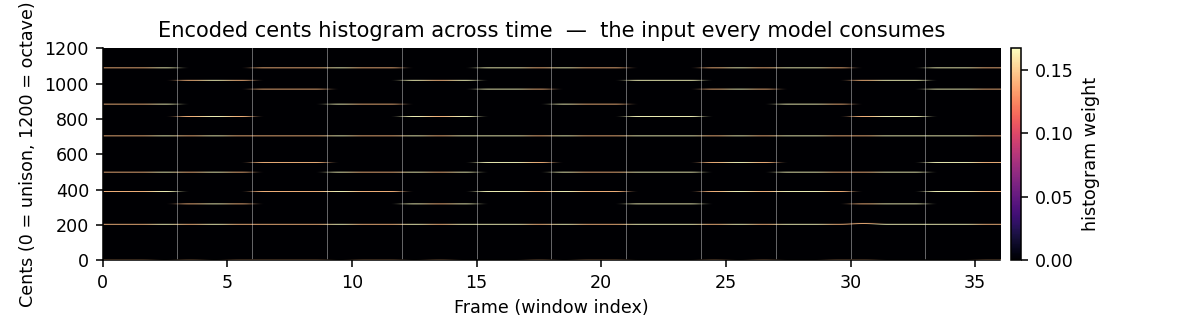
\includegraphics[width=\linewidth]{00_input_histograms}
  \caption{Encoded cents histograms across 36 frames. White vertical
  lines mark ground-truth regime changes (every 3 frames). Horizontal
  ridges correspond to JI intervals (perfect fifth at $\approx702$\,¢,
  octave at 1200\,¢). The shifting ridges between blocks reveal the
  harmonic motion that each approach decomposes differently.}
  \label{fig:input}
\end{figure}

% ─────────────────────────────────────────────────────────────────────────────
\part{Per-approach explanations}
% ─────────────────────────────────────────────────────────────────────────────

\section{HarmonicMarkov --- discrete-state dynamics}

\begin{insight}
Sort every window into one of $K$ ``harmonic moods'' (states), then
build a table of probabilities for moving from mood $i$ to mood $j$.
\end{insight}

K-means clusters the $(T\times n_{\text{bins}})$ histograms into $K$
discrete harmonic states; a first- (or higher-) order Markov chain is
estimated from the resulting label sequence. With
\texttt{n\_states='auto'}, $K$ is chosen by silhouette score across a
configurable range.

\paragraph{Question it answers.}  \emph{How many harmonic ``modes'' does
this recording inhabit, how long does it stay in each, and how
predictable is the next mode given the current one?}

\begin{outputbox}
\begin{itemize}[nosep,leftmargin=*]
  \item \textbf{Transition matrix} --- which states are adjacent.
  \item \textbf{Stationary distribution} --- the harmonic ``home base''.
  \item \textbf{Transition entropy} $\in [0, \log_2 K]$ --- low for stable
        recordings, high for unpredictable ones.
  \item \textbf{Cluster centres} --- prototype tunings, directly playable
        via the render bridge.
\end{itemize}
\end{outputbox}

\begin{usecasebox}
\textbf{Neural state dynamics:} cluster EEG into harmonic states during
rest vs.\ task; compare dwell times, transition rates and entropy.
\textbf{Pharmacological state shifts:} the steady-state distribution is
a fingerprint of the attractor, not just the average metric.
\textbf{Generative tuning prototypes:} cluster centroids are valid cents
histograms; export as a small vocabulary of prototype tunings.
\end{usecasebox}

\begin{figure}[H]
  \centering
  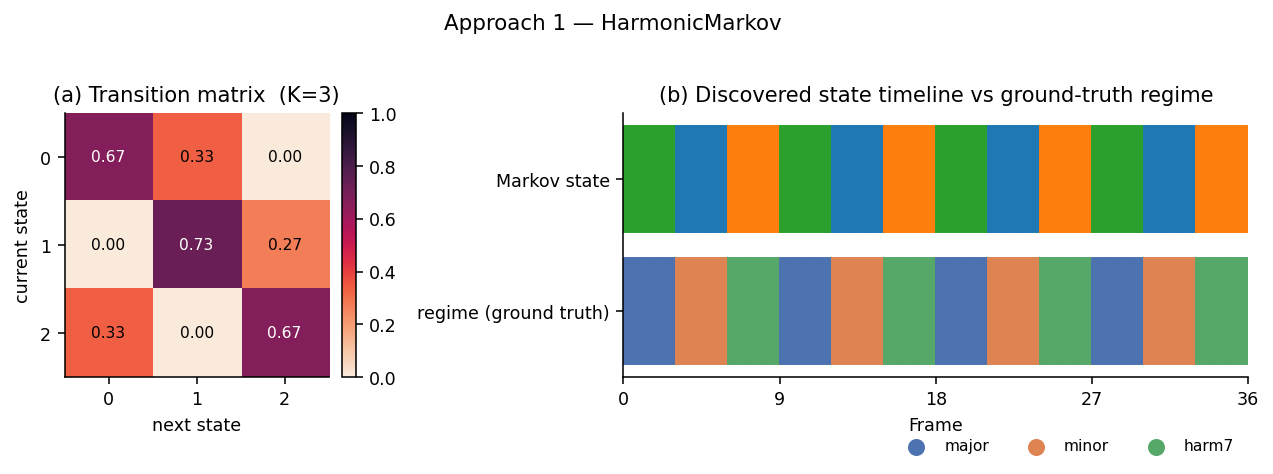
\includegraphics[width=\linewidth]{01_markov}
  \caption{(a) Transition matrix learned from histogram clusters. Each
  row sums to 1. (b) Discovered Markov state per frame (top) vs.\
  ground-truth regime (bottom). The model recovers the three-regime
  cycle with no supervision, and the matrix is dominated by
  $0\!\to\!1\!\to\!2\!\to\!0$ cyclic structure.}
  \label{fig:markov}
\end{figure}

\begin{cavbox}
Needs $T \gtrsim 5K$ for meaningful estimates. \texttt{n\_states='auto'}
can pick large $K$ when tiny drift makes every frame its own cluster
--- set a tight \texttt{auto\_k\_range} when a small number of regimes
is expected. Assumes a discrete-state geometry; use
\texttt{HarmonicLatentSpace} for continuous manifolds.
\end{cavbox}

% ─────────────────────────────────────────────────────────────────────────────
\section{WassersteinTrajectory --- harmonic motion}

\begin{insight}
Picture each window's cents-histogram as sand on the cents axis. The
\emph{Earth Mover's Distance} is the minimum work to reshape one pile
into another. \emph{Flux} is that work between consecutive windows ---
a moment-to-moment harmonic velocity in cents-units.
\end{insight}

The 1-D Wasserstein-1 distance equals the $L^1$ distance of cumulative
distribution functions. The flux vector
$\phi_t = W_1(\mathbf{h}_t, \mathbf{h}_{t+1})$, the pairwise matrix
$D_{ij} = W_1(\mathbf{h}_i, \mathbf{h}_j)$, and quantile-space
barycentric interpolation all follow without modification across
representations.

\paragraph{Question it answers.}  \emph{How fast is the harmonic content
changing, when does it change, and which windows are nearest neighbours
in interval space?}

\begin{outputbox}
\begin{itemize}[nosep,leftmargin=*]
  \item \textbf{Flux} $\phi_t$ --- locates transitions; peaks mark
        moments of harmonic reorganisation.
  \item \textbf{Pairwise matrix} --- block-banded structure reveals
        stable episodes and recurrent states.
  \item \textbf{Barycenter interpolation} --- musically valid glissandi
        between any two frames; decodes directly to MIDI.
  \item \textbf{MDS/UMAP embedding} --- session topology in 2-D for
        nearest-neighbour retrieval.
\end{itemize}
\end{outputbox}

\begin{usecasebox}
\textbf{Transition detection:} flag stimulus onsets, drug bolus, micro-arousals
via $z(\phi_t)>2$. \textbf{Session fingerprint:} mean / std flux is a
per-recording signature (meditation low, cognitive task high).
\textbf{Smooth glissandi:} \texttt{interpolate\_pair} produces a path
suitable for the MIDI bridge.
\end{usecasebox}

\begin{figure}[H]
  \centering
  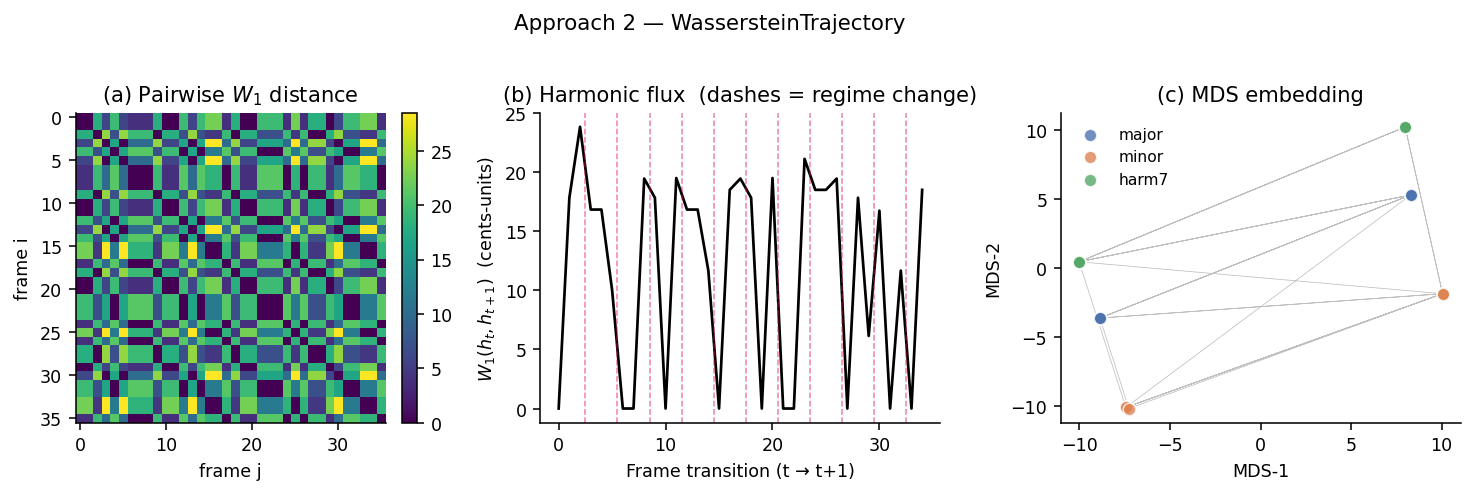
\includegraphics[width=\linewidth]{02_wasserstein}
  \caption{(a) Pairwise $W_1$ matrix. The checkerboard pattern with
  period 3 reflects the regime cycle. (b) Flux time series. Peaks
  coincide almost perfectly with ground-truth regime changes. (c) MDS
  embedding collapses the trajectory to three clusters --- the three
  regimes are recovered as discrete manifold locations.}
  \label{fig:wass}
\end{figure}

\begin{cavbox}
$\mathcal{O}(T^2 \cdot n_{\text{bins}})$ memory and $\mathcal{O}(T^2)$
wall time. For very long recordings, downsample or work block-wise. $W_1$
on cents treats the axis as Euclidean; octave-equivalence (circular
ground space) is not built in.
\end{cavbox}

% ─────────────────────────────────────────────────────────────────────────────
\section{HarmonicDMD --- linear dynamical modes}

\begin{insight}
DMD assumes a hidden linear clock $\mathbf{x}_{t+1} \approx A\mathbf{x}_t$
and factors it into independent oscillating modes, each with its own
frequency and growth/decay rate.
\end{insight}

Exact DMD: an SVD-truncated pseudoinverse fits the operator $A$ to the
snapshot pair $(X_{:T-1}, X_{1:})$, and the eigenvalues/modes of $A$
classify the dynamics. Eigenvalues inside $|\lambda|=1$ decay; on it,
oscillate at $\arg\lambda$; outside, grow.

\begin{outputbox}
\begin{itemize}[nosep,leftmargin=*]
  \item \textbf{Eigenvalues} --- spectrum on the complex plane;
        modes near the unit circle are persistent oscillators.
  \item \textbf{Growth rates} $\mathrm{Re}\log\lambda$ ---
        destabilising trends worth flagging.
  \item \textbf{Frequencies} $\mathrm{Im}\log\lambda$ --- timescales
        of recurring cycles in windows-per-cycle units.
  \item \textbf{Reconstruction} --- forward extrapolation from the
        last fitted state.
\end{itemize}
\end{outputbox}

\begin{usecasebox}
\textbf{Detecting harmonic oscillations:} respiration- or
heart-rate-driven modulation of EEG harmonic content.
\textbf{Short-term forecasting:} a sanity baseline against ML predictors.
\textbf{Stress/relaxation classification:} growth-rate distributions
differ across conditions.
\end{usecasebox}

\begin{figure}[H]
  \centering
  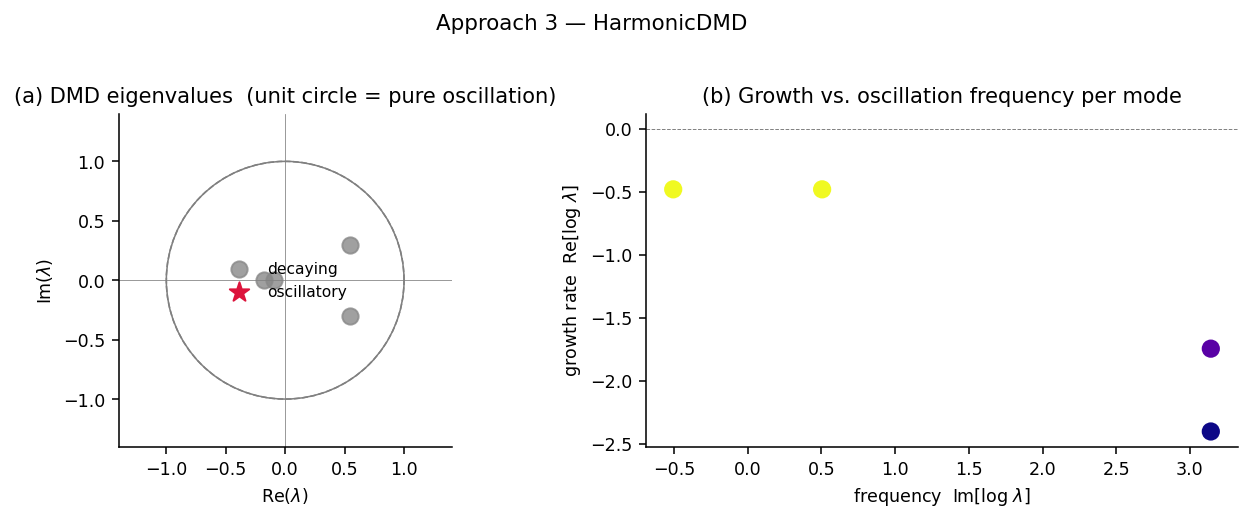
\includegraphics[width=\linewidth]{03_dmd}
  \caption{(a) Complex-plane scatter of DMD eigenvalues; grey points
  decay, the red star is the slowest-decaying mode. (b) Growth rate vs.\
  frequency, coloured by $|\lambda|$.}
  \label{fig:dmd}
\end{figure}

\begin{cavbox}
DMD assumes uniform time steps. When only ratio lists are available
(no scalar metrics), use \texttt{use\_histograms=True}; with $T<30$ the
eigenvalue spectrum is unreliable.
\end{cavbox}

% ─────────────────────────────────────────────────────────────────────────────
\section{HarmonicLatentSpace --- continuous harmonic manifold}

\begin{insight}
PCA finds the directions in feature space along which harmonic content
varies most across windows. The trajectory's shape (cluster, arc, loop)
immediately reveals temporal structure.
\end{insight}

A linear PCA gives \texttt{encode}/\texttt{decode}, a smooth
$(T \times \texttt{latent\_dim})$ trajectory, and per-axis explained
variance. It is the continuous-state counterpart of
\texttt{HarmonicMarkov}.

\begin{outputbox}
\begin{itemize}[nosep,leftmargin=*]
  \item \textbf{Trajectory} --- the path through PC space; shape
        diagnoses dynamics.
  \item \textbf{Scree} --- effective dimensionality of the harmonic
        manifold.
  \item \textbf{Interpolation} --- continuous morphs between any two
        recorded states; decoded histograms are playable.
\end{itemize}
\end{outputbox}

\begin{usecasebox}
\textbf{Compact session summary:} a $T$-frame recording compresses to a
$(T\times 3)$ trajectory. \textbf{Cross-session alignment:} two sessions
in the same PCA basis become directly comparable as paths. \textbf{Brain-state
morphing:} \texttt{interpolate} between any two latent points generates
microtonal morphs.
\end{usecasebox}

\begin{figure}[H]
  \centering
  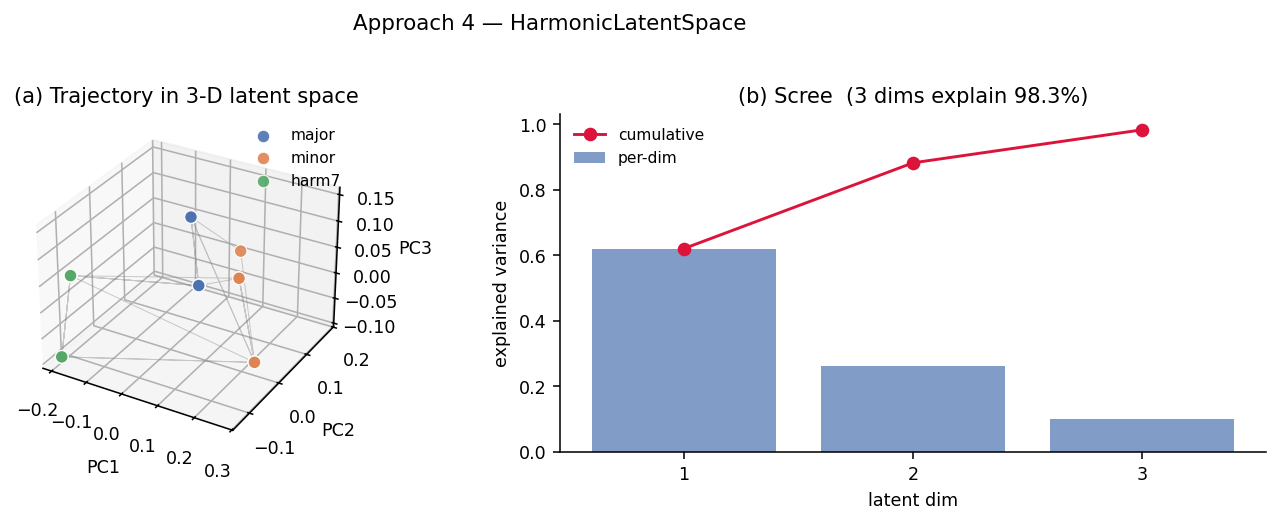
\includegraphics[width=\linewidth]{04_latent}
  \caption{(a) Trajectory in the first 3 PCs, coloured by ground-truth
  regime. (b) Scree plot --- 3 dimensions explain 98\,\% of the
  histogram variance, indicating low intrinsic dimensionality.}
  \label{fig:latent}
\end{figure}

\begin{cavbox}
PCA is linear; for non-linear manifolds, consider the MDS embedding from
\texttt{WassersteinTrajectory}. Very small components may decode to
all-zero histograms --- filter peaks with \texttt{prominence}.
\end{cavbox}

% ─────────────────────────────────────────────────────────────────────────────
\section{HarmonicTopology --- shape of the trajectory}

\begin{insight}
Topology asks: \emph{what is the shape of the data?} Takens delay
embedding turns a scalar harmonicity series into a point cloud; persistent
homology counts connected components ($\beta_0$) and loops ($\beta_1$) as
the inflation radius grows.
\end{insight}

H0 (always available via scipy linkage) counts harmonic basins; H1
(requires \texttt{ripser}) catches cyclic progressions. The 6-element
\emph{session fingerprint} (mean / max persistence and bar count for
each dimension) compactly summarises an entire recording.

\begin{outputbox}
\begin{itemize}[nosep,leftmargin=*]
  \item \textbf{Betti numbers} $\beta_0, \beta_1$ --- count attractors
        and loops.
  \item \textbf{Persistence diagram} --- detailed multi-scale view.
  \item \textbf{Session fingerprint} --- fixed 6-vector for
        comparing recordings.
\end{itemize}
\end{outputbox}

\begin{usecasebox}
\textbf{Attractor counting:} how many distinct harmonic basins did the
recording visit? \textbf{Cycle detection:} persistent H1 = robust harmonic
loop (distinct from DMD's linear oscillation).
\textbf{Session fingerprinting:} 6-vector comparable across recordings
and subjects.
\end{usecasebox}

\begin{figure}[H]
  \centering
  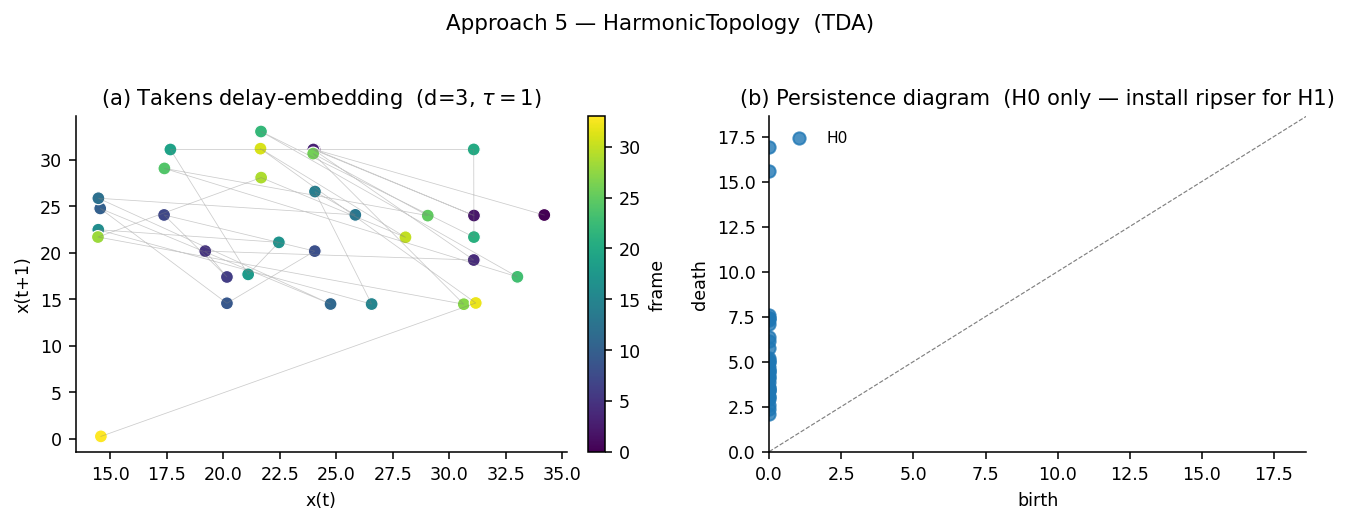
\includegraphics[width=\linewidth]{05_topology}
  \caption{(a) 2-D projection of the 3-D Takens cloud, coloured by
  frame. The cloud's discrete structure flags attractor basins. (b) H0
  persistence diagram --- points far from the diagonal are long-lived
  components. With \texttt{ripser} installed, an H1 series appears for
  loop detection.}
  \label{fig:topo}
\end{figure}

\begin{cavbox}
Without \texttt{ripser}, only H0 is available --- no loop detection.
Choice of \texttt{scalar\_key} matters enormously; \texttt{'harmsim'} is
the canonical default.
\end{cavbox}

% ─────────────────────────────────────────────────────────────────────────────
\section{HarmonicGrammar --- symbolic chord language}

\begin{insight}
Treat each window's ratios as a \emph{word} in a harmonic language. Each
ratio is mapped to its closest named JI interval, the window becomes a
chord token, and an N-gram model learns conditional probabilities.
\end{insight}

The grammar is intrinsically cents-based --- it relies on the JI
interval dictionary. Outputs include a vocabulary of distinct chord
tokens, an N-gram transition table, top motifs, and a Levenshtein
distance for comparing symbolic sequences across recordings.

\begin{outputbox}
\begin{itemize}[nosep,leftmargin=*]
  \item \textbf{Vocabulary} --- the chord types this recording uses.
  \item \textbf{Top motifs} --- recurring chord progressions
        (``riffs'' of the biosignal).
  \item \textbf{Transition entropy} --- chord-level predictability.
  \item \textbf{Levenshtein} --- edit distance between two
        chord sequences.
\end{itemize}
\end{outputbox}

\begin{usecasebox}
\textbf{Symbolic biosignal fingerprint:} two recordings compared by
edit distance over their chord-token streams. \textbf{Motif discovery:}
\texttt{top\_motifs} surfaces recurring progressions as resonance /
entrainment candidates. \textbf{Predictability measure:} N-gram entropy
is a chord-level Lempel--Ziv complexity score.
\end{usecasebox}

\begin{figure}[H]
  \centering
  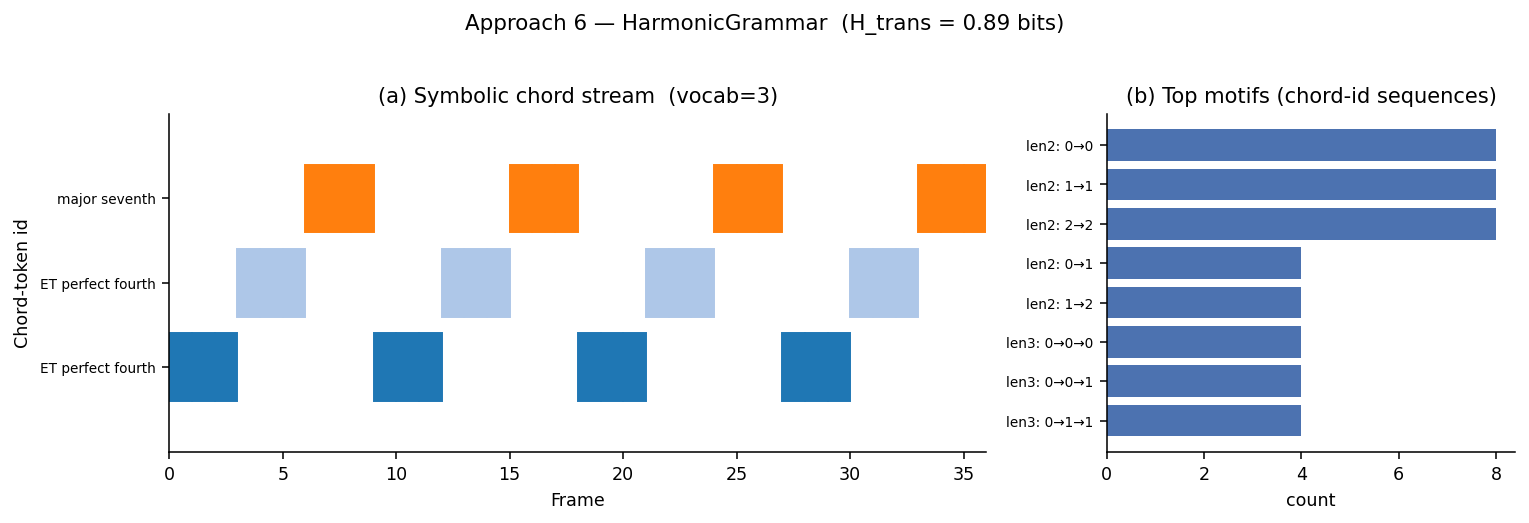
\includegraphics[width=\linewidth]{06_grammar}
  \caption{(a) Symbolic chord stream over 36 frames; the three regimes
  collapse to three distinct chord tokens at the configured 30\,¢
  tolerance. (b) Top motifs: length-2 self-loops dominate because each
  regime persists for 3 frames; remaining motifs encode the
  $0\!\to\!1\!\to\!2$ cycle.}
  \label{fig:grammar}
\end{figure}

\begin{cavbox}
A chord is a \emph{set}, not a multiset --- two ratios mapped to the
same JI label collapse to one symbol. \texttt{tolerance\_cents} is a
hyperparameter that shapes vocabulary size; report it explicitly.
\end{cavbox}

% ─────────────────────────────────────────────────────────────────────────────
\section{The rendering bridge --- closing the loop}

Once a model produces a histogram (or a sequence of them), the bridge
layer (\texttt{histogram\_to\_ratios}, \texttt{histogram\_to\_scl},
\texttt{histograms\_to\_midi}) maps it back to playable tunings.
\texttt{analyzer.get\_histograms(source=...)} dispatches across
\texttt{observed}, \texttt{wasserstein\_interp}, \texttt{latent\_interp},
\texttt{markov\_centroids}, \texttt{markov\_sample}, \texttt{dmd\_predict}.

\begin{figure}[H]
  \centering
  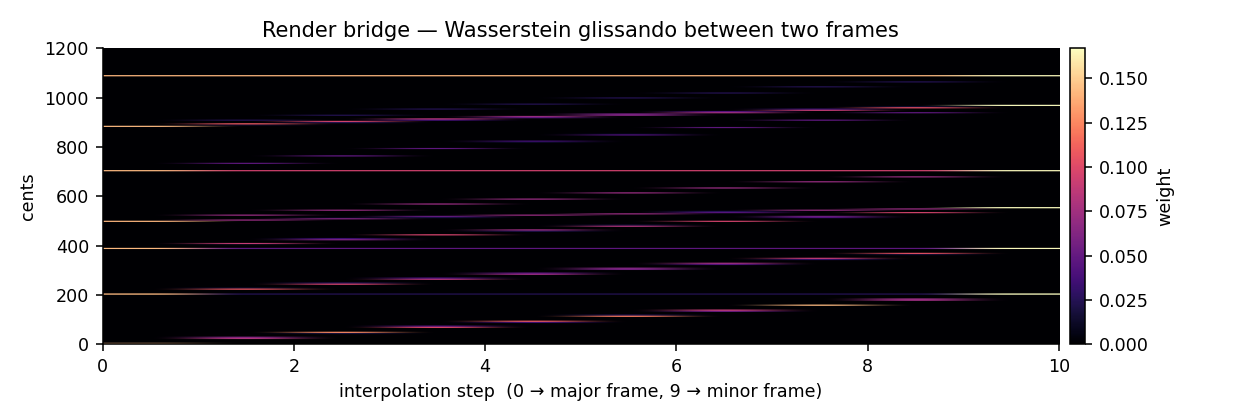
\includegraphics[width=\linewidth]{07_bridge_glissando}
  \caption{Ten-step Wasserstein quantile-space interpolation between a
  major-regime frame and a minor-regime frame. Stable intervals
  (unison, fifth, octave) stay fixed; the moving notes (major-third
  $\to$ minor-third, major-sixth $\to$ minor-sixth) drift smoothly. The
  result is a microtonal glissando, exportable as MIDI.}
  \label{fig:bridge}
\end{figure}

The bridge is intentionally locked to the \texttt{cents\_histogram}
representation: the harmonicity-spectrum and -matrix representations
live in spectrum-space and cannot be inverted to ratios. The analyser
raises a clear \texttt{RuntimeError} if a generative source is requested
on a non-cents representation.

% ─────────────────────────────────────────────────────────────────────────────
\section{When to use which approach}

\begin{table}[H]
\centering
\small
\begin{tabular}{@{}p{0.42\linewidth}p{0.27\linewidth}p{0.27\linewidth}@{}}
\toprule
\textbf{Question} & \textbf{Approach} & \textbf{Output} \\
\midrule
``How many harmonic modes? How long is each held?''
  & HarmonicMarkov     & Transition matrix, dwell-time, $\boldsymbol\pi$ \\
``When does harmonic content change, by how much?''
  & WassersteinTrajectory & Flux, distance matrix, embedding \\
``Is there oscillatory dynamics? At what timescale?''
  & HarmonicDMD        & Eigenvalues, modes, forecast \\
``What is the trajectory through harmonic space?''
  & HarmonicLatentSpace & 3-D path, scree, interpolation \\
``How many attractor basins / loops in the trajectory?''
  & HarmonicTopology    & $\beta_0, \beta_1$, 6-vector fingerprint \\
``What chord vocabulary / motifs / predictability?''
  & HarmonicGrammar     & Vocabulary, top n-grams, edit distance \\
\bottomrule
\end{tabular}
\caption{Decision rubric: questions $\to$ approaches.}
\end{table}

A typical workflow is:
\begin{enumerate}[nosep,leftmargin=*]
  \item Inspect \texttt{analyzer.summary()} for a health check.
  \item Look at the \textbf{Wasserstein flux} to identify \emph{when}
        something happens.
  \item Use the \textbf{Markov} matrix to ask \emph{between which modes}.
  \item Use the \textbf{Latent} trajectory for a continuous view; then
        \textbf{Topology} to test discreteness vs.\ continuity (via
        $\beta_0, \beta_1$).
  \item Use the \textbf{Grammar} to attach human-readable chord labels
        to the structure the geometry exposed.
  \item Use \textbf{DMD} when oscillatory dynamics are suspected.
\end{enumerate}

% ─────────────────────────────────────────────────────────────────────────────
\part{Showcase across qualitatively distinct dynamics}
% ─────────────────────────────────────────────────────────────────────────────

\section{Five scenarios with biosignal motivations}

Part~I introduced each approach on a single sequence. To show what each
model \emph{actually distinguishes}, we run the pipeline across five
qualitatively different scenarios, each motivated by a real biosignal
recording type:

\begin{table}[H]
\centering
\small
\begin{tabular}{@{}llp{0.49\linewidth}@{}}
\toprule
\textbf{Scenario} & \textbf{Construction} & \textbf{Motivating biosignal} \\
\midrule
A. Stable      & Same just-major tuning + noise, $T=32$
               & meditation baseline, sleep N3, isoflurane plateau \\
B. Drift       & Linear interp.\ major$\to$minor, $T=32$
               & slow anaesthesia induction, sleep-stage transition \\
C. Cycle       & 3 regimes cycling every 9 frames, $T=36$
               & repetitive motor task, periodic chord progression \\
D. Oscillation & Sinusoidal blend major$\leftrightarrow$minor, period 8, $T=48$
               & breathing-driven harmonic modulation, slow alpha envelope \\
E. Perturbed   & Stable + abrupt switch at frame 24, $T=40$
               & stimulus onset, drug bolus, seizure onset, micro-arousal \\
\bottomrule
\end{tabular}
\caption{The five scenarios used in Parts II--III, and the recording
type each is constructed to mimic. The unison (1.0) is excluded from
all bases --- under noise it would drift across the cents=0 histogram
boundary and contaminate the comparison.}
\end{table}

\section{Four signatures at a glance}

\begin{figure}[H]
  \centering
  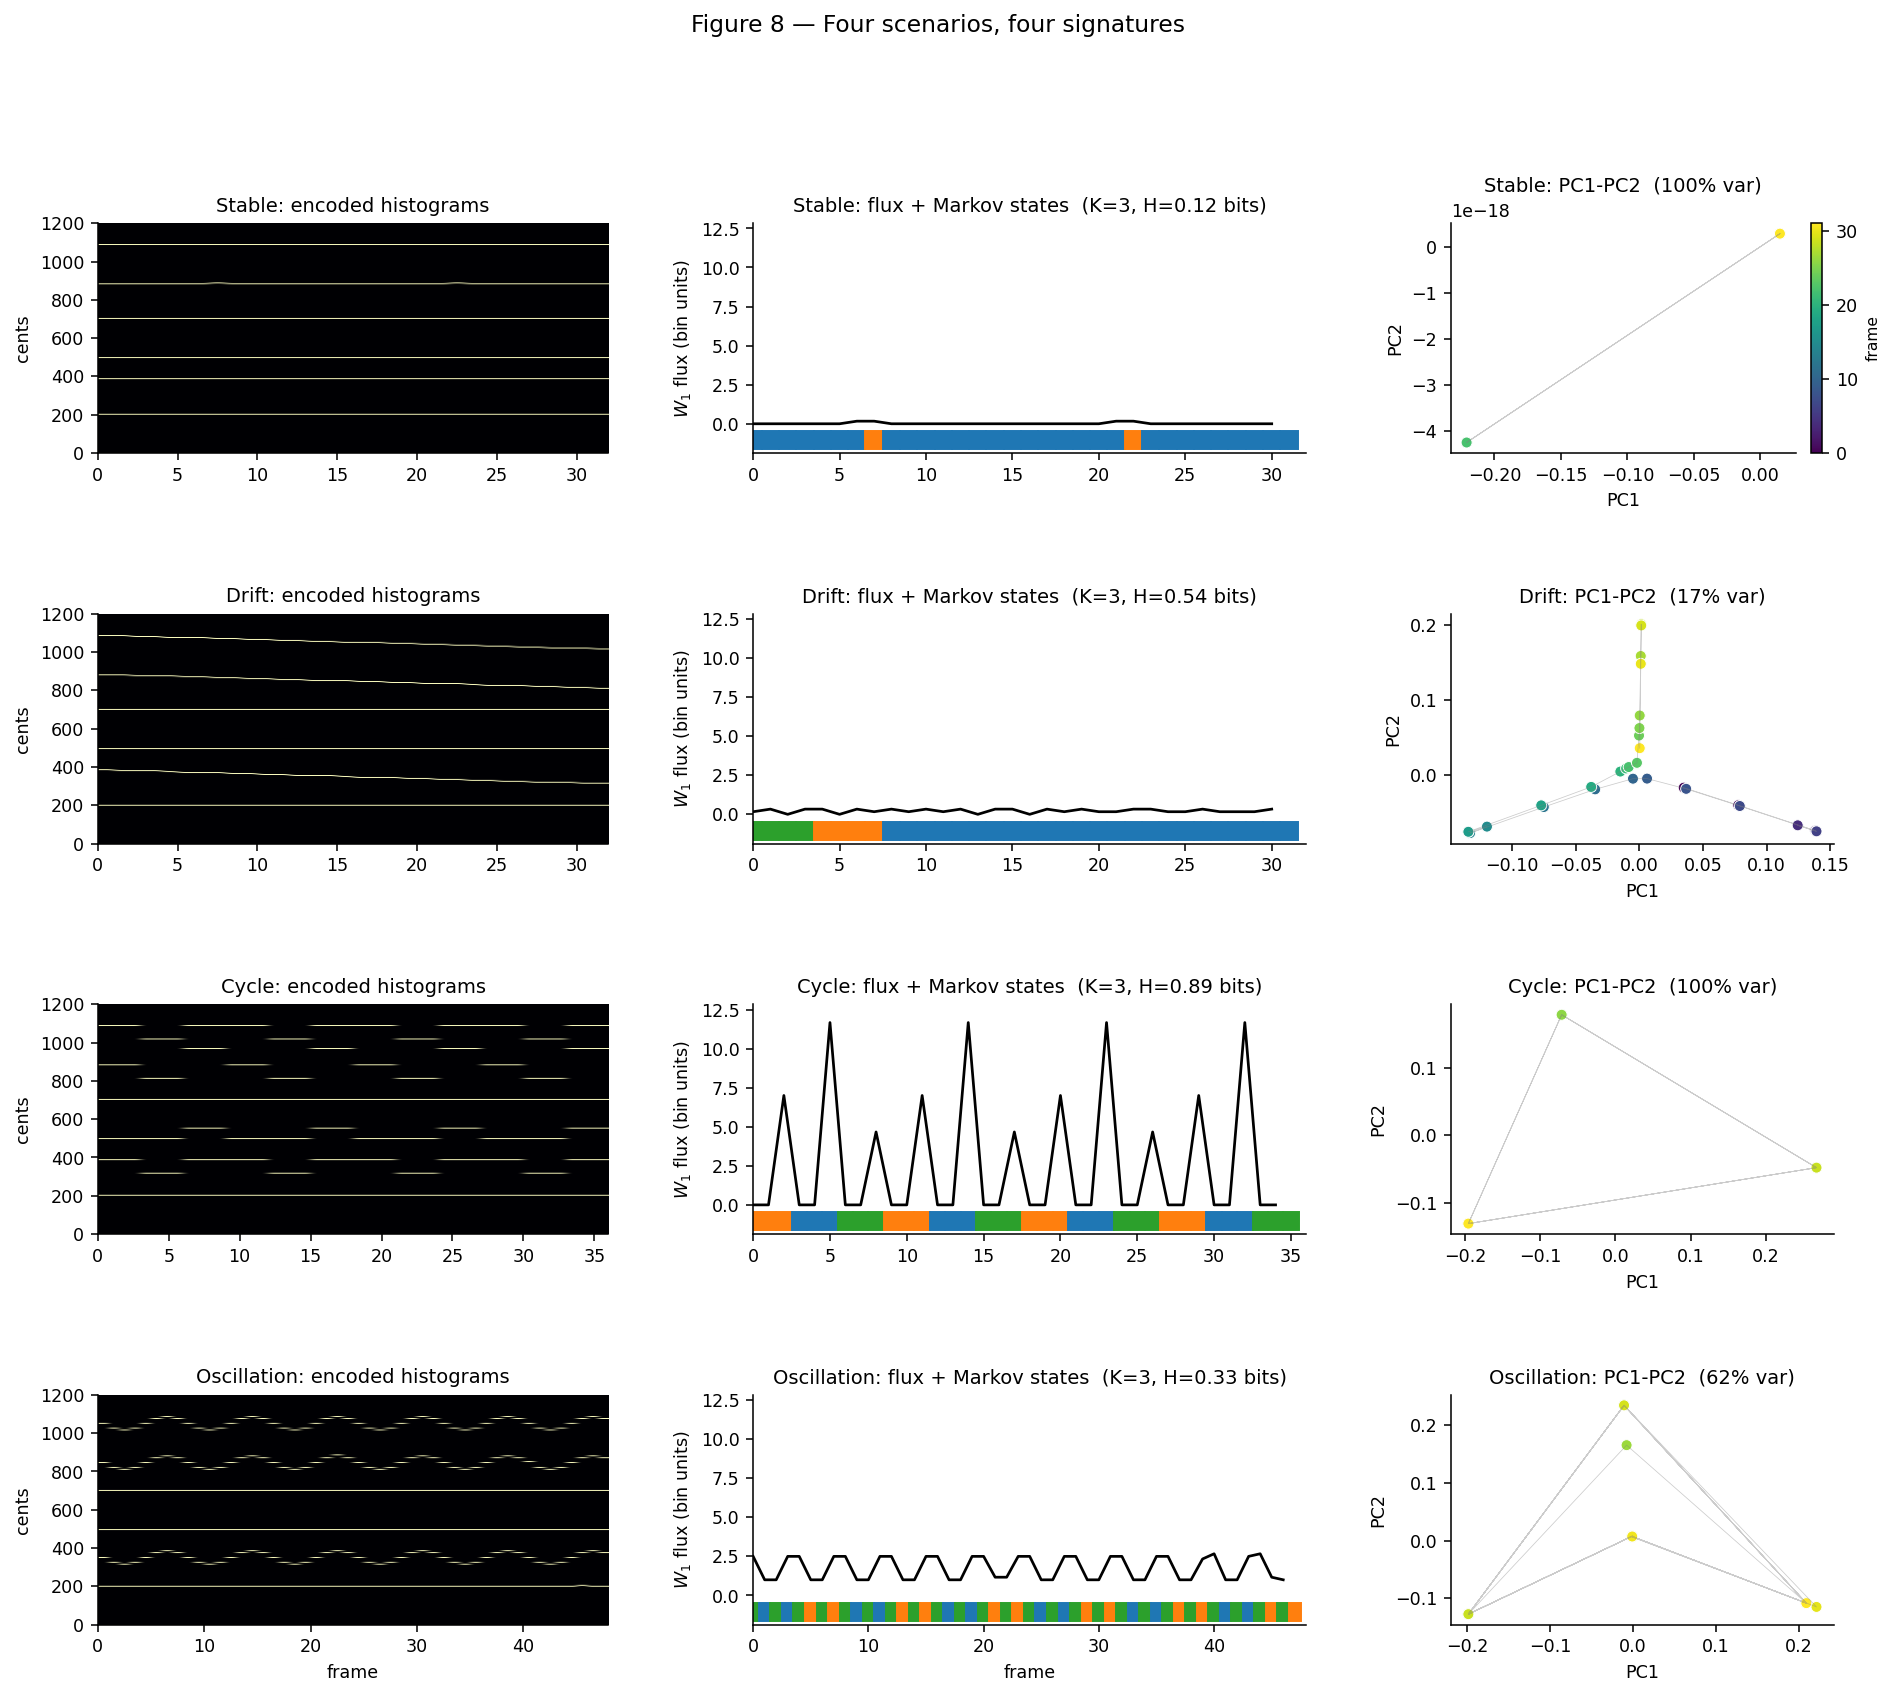
\includegraphics[width=\linewidth]{08_scenarios_overview}
  \caption{Four scenarios (rows) $\times$ three lenses (columns). All
  rows use the \textbf{same K=3 Markov fit} for apples-to-apples
  comparison; the $W_1$ flux y-axis is shared across rows. The
  qualitative signature of each scenario is immediately readable: low
  flux \& near-zero Markov entropy for Stable; smooth curved PCA arc
  for Drift; periodic flux spikes \& three discrete PCA clusters for
  Cycle; sinusoidal flux \& elliptical PCA orbit for Oscillation.}
  \label{fig:scenarios}
\end{figure}

\textbf{The key observation:} no single column would have made these
scenarios clearly distinguishable. The combination of flux pattern,
Markov entropy, and PCA shape gives each scenario a unique signature.

\section{DMD on an oscillatory recording}

The Oscillation scenario is the natural showcase for DMD: it is by
construction a low-rank linear dynamical system with an 8-frame period.

\begin{figure}[H]
  \centering
  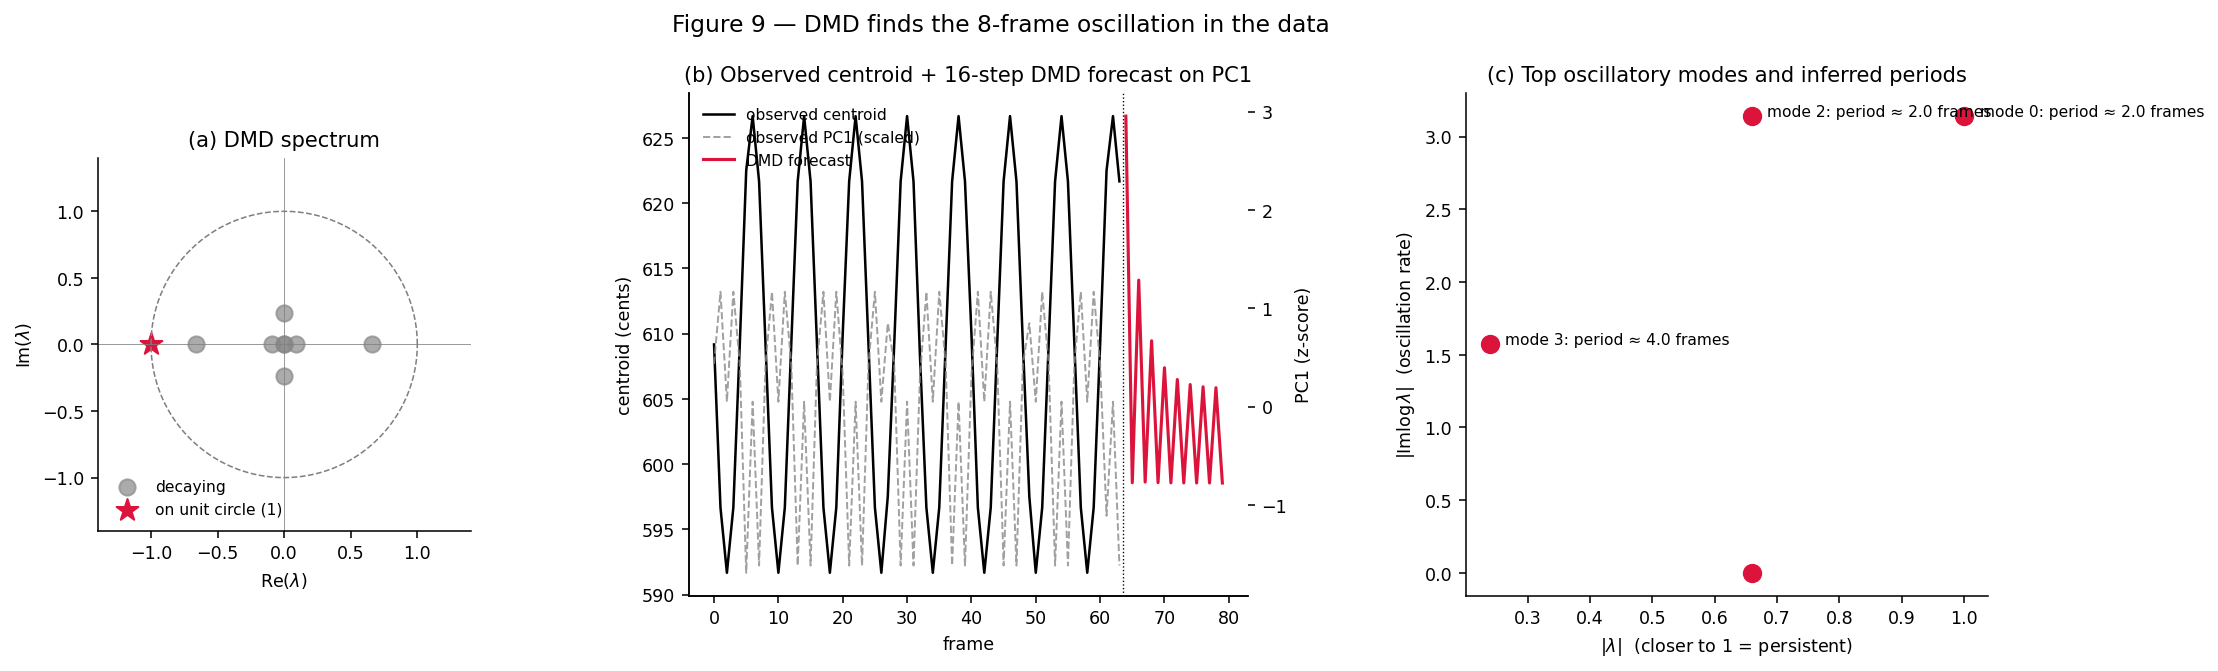
\includegraphics[width=\linewidth]{09_dmd_oscillation}
  \caption{DMD on a 64-frame period-8 oscillation. (a) Most eigenvalues
  decay; one sits essentially on the unit circle (red star) --- the
  slow-decaying oscillatory mode. (b) Observed centroid-of-cents
  overlaid with the first principal component; the DMD 16-step forecast
  continues the oscillation past the data. (c) Top-4 modes ranked by
  $||\lambda|-1|$, with inferred periods.}
  \label{fig:dmdosc}
\end{figure}

\section{Topology distinguishes shape, not magnitude}

\begin{figure}[H]
  \centering
  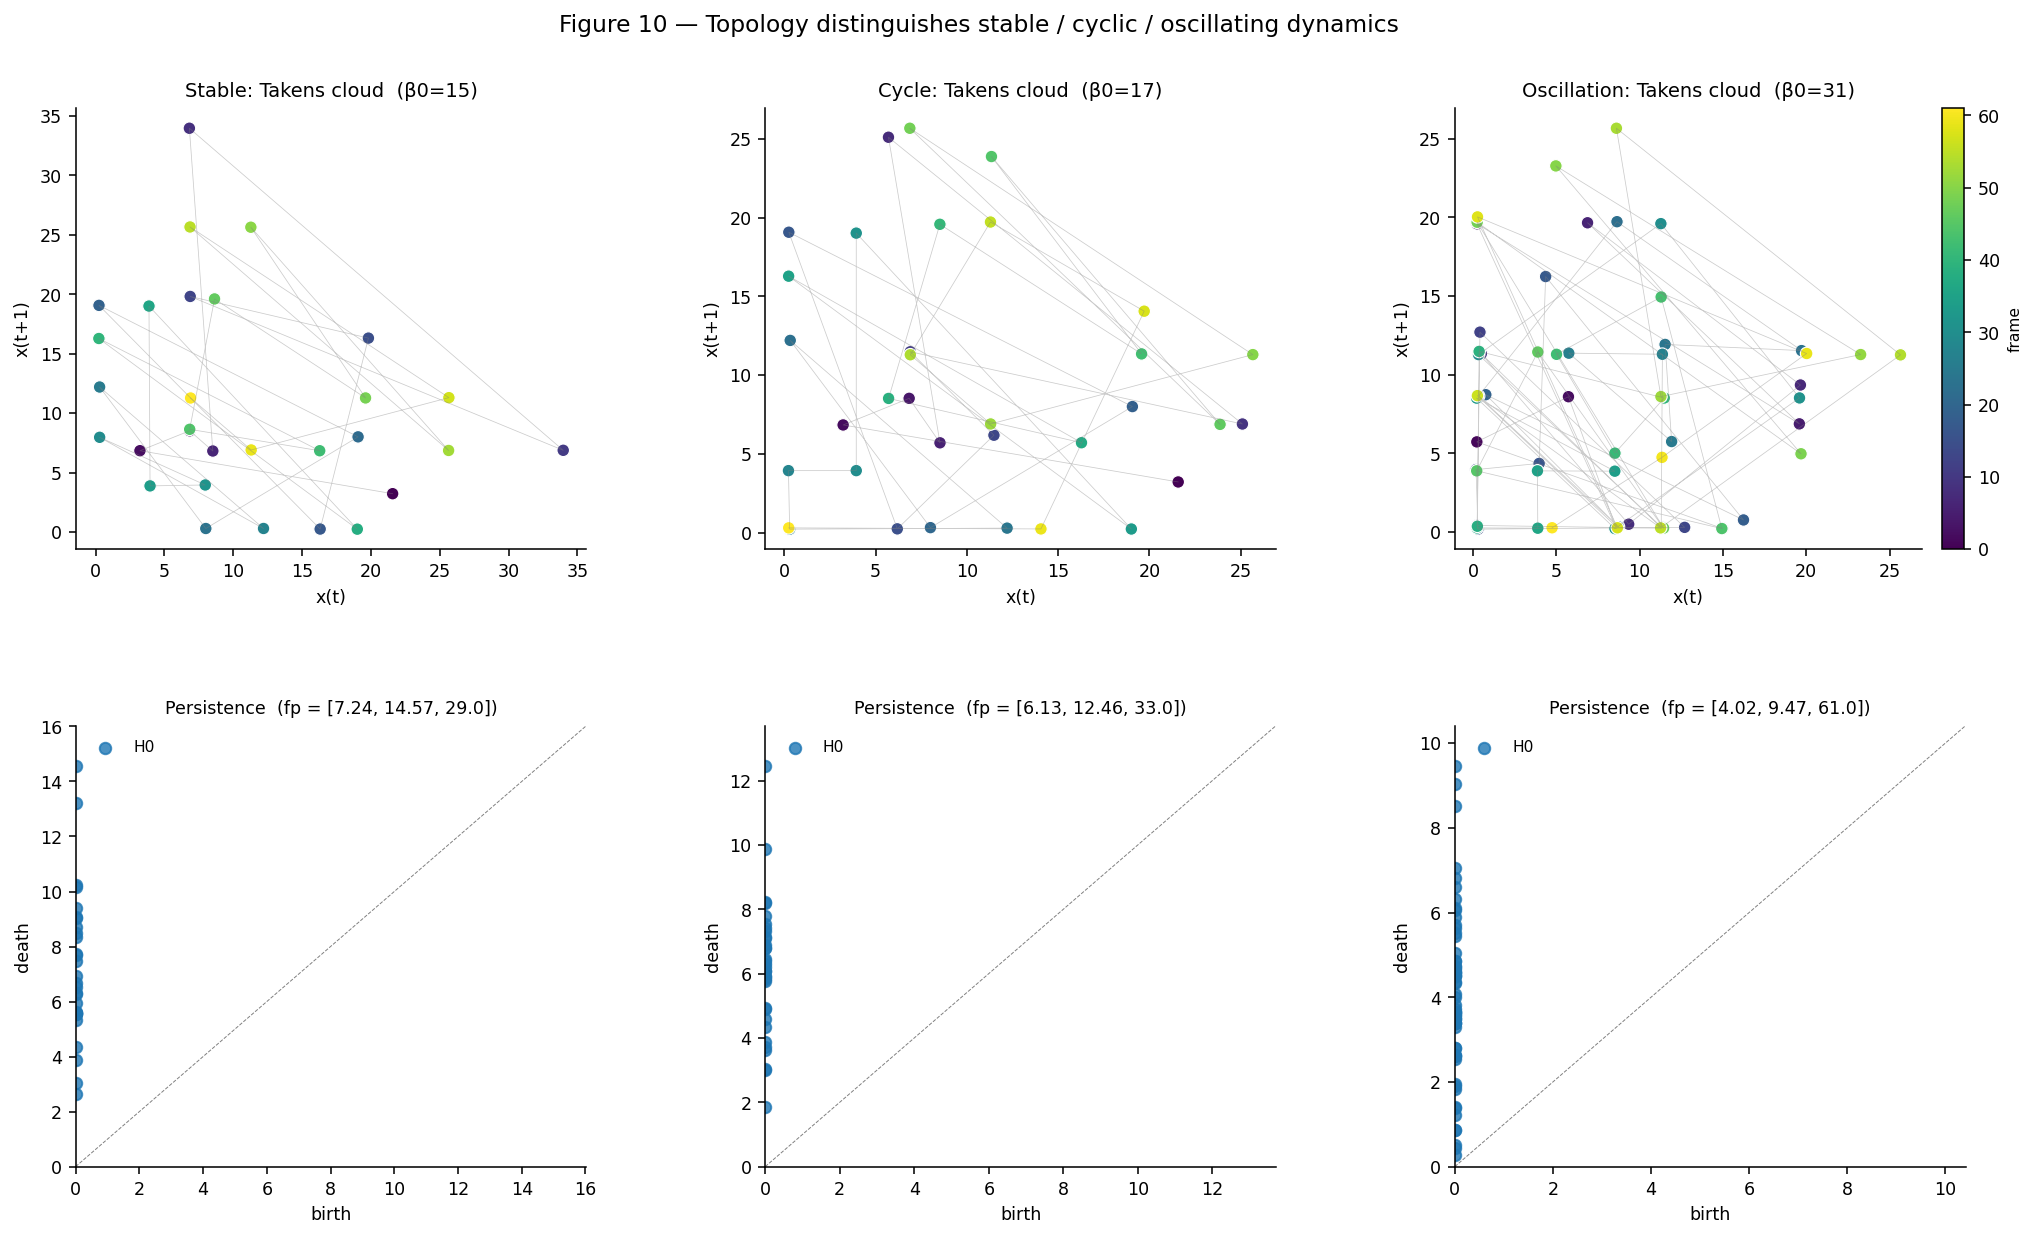
\includegraphics[width=\linewidth]{10_topology_scenarios}
  \caption{Takens embedding of the \texttt{harmsim} series for three
  scenarios. \textbf{Stable:} cloud collapses near a line.
  \textbf{Cycle:} cloud breaks into discrete clusters (attractor
  basins). \textbf{Oscillation:} cloud forms a loop-like structure ---
  with \texttt{ripser}, a persistent H1 bar would appear as
  topological proof of cyclic dynamics.}
  \label{fig:toposcen}
\end{figure}

% ─────────────────────────────────────────────────────────────────────────────
\part{End-to-end applications}
% ─────────────────────────────────────────────────────────────────────────────

\section{Application: event detection from harmonic flux}

\paragraph{Question.}  Given a streamed biosignal segmented into windows,
can we flag when something \emph{happens} without supervised labels?

\paragraph{Pipeline.}  Encode histograms $\to$ flux $\to$ z-score
$\to$ threshold at $z>2\sigma$; cross-validate against Markov state
labels.

\begin{figure}[H]
  \centering
  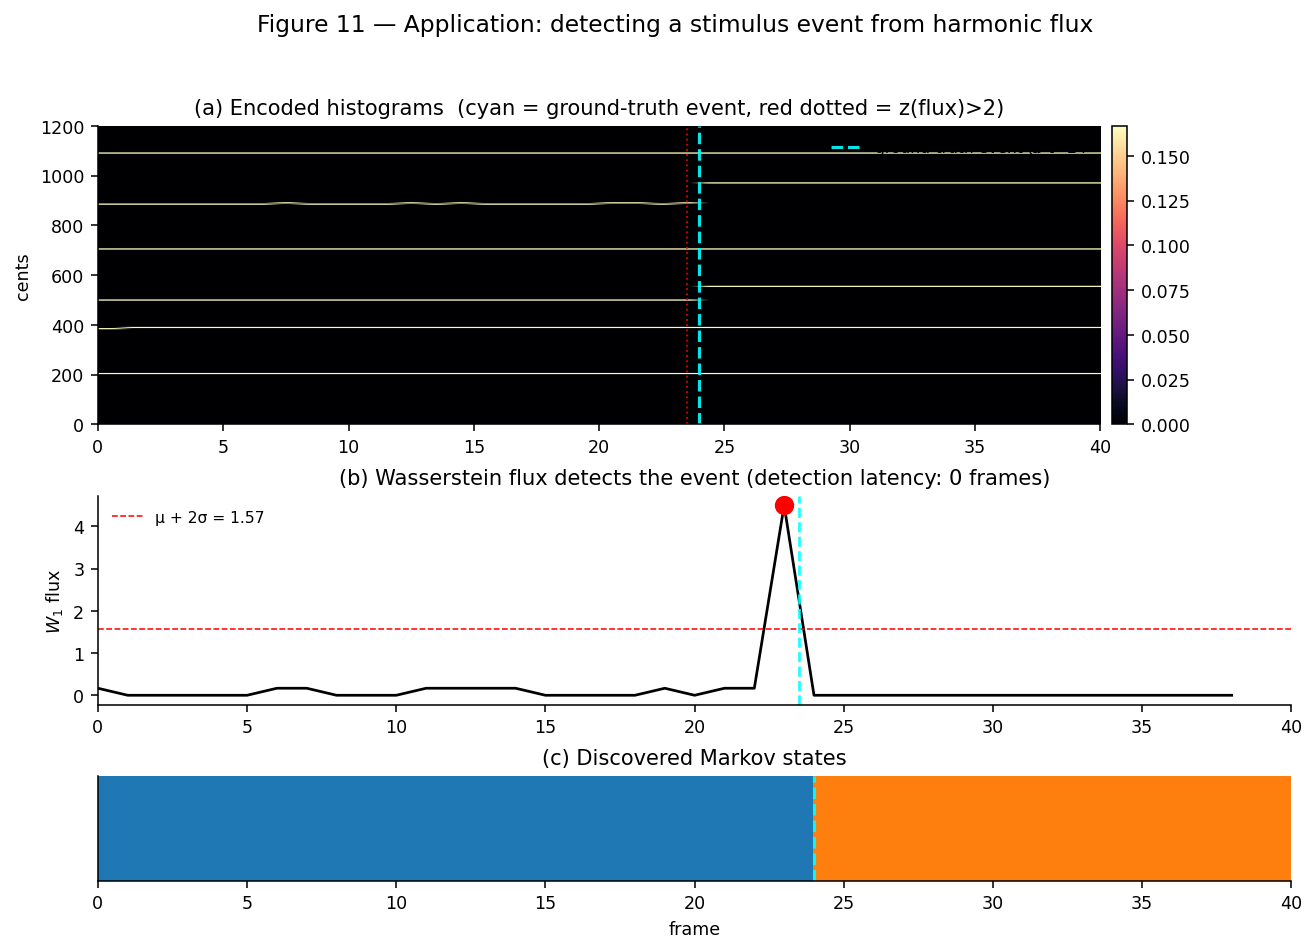
\includegraphics[width=\linewidth]{11_application_event_detection}
  \caption{Perturbed scenario: 24 frames of stable just-major, then an
  abrupt switch to harmonic-7. (a) Histogram heatmap; cyan dashed =
  ground truth, red dotted = $z(\phi)>2$ detection. (b) Flux is
  $\approx 0$ throughout the stable epoch then \textbf{spikes to
  $\approx 4.5$} at the event --- the detector triggers once, with
  \emph{zero latency}. (c) The K=2 Markov chain partitions the timeline
  cleanly at the transition.}
  \label{fig:event}
\end{figure}

\begin{usecasebox}
\textbf{Online flagging:} continuous EEG monitoring with z-threshold
state-change alerts. \textbf{Unsupervised stimulus-onset detection} in
long recordings with unreliable event logs.
\textbf{Quality control:} single-frame artefacts as outlier flux spikes.
\end{usecasebox}

\section{Application: per-recording fingerprinting}

\paragraph{Question.}  Can we extract a fixed-length descriptor that
distinguishes recording \emph{types}, suitable for clustering /
classification?

\paragraph{Pipeline.}  \texttt{analyzer.fit\_all()} $\to$ assemble an
8-vector
$[\bar\phi,\sigma_\phi, K, H_{\text{markov}}, \text{var}_{PC1+2},
\beta_0, f_{\text{osc}}, H_{\text{grammar}}]$ per recording.

\begin{figure}[H]
  \centering
  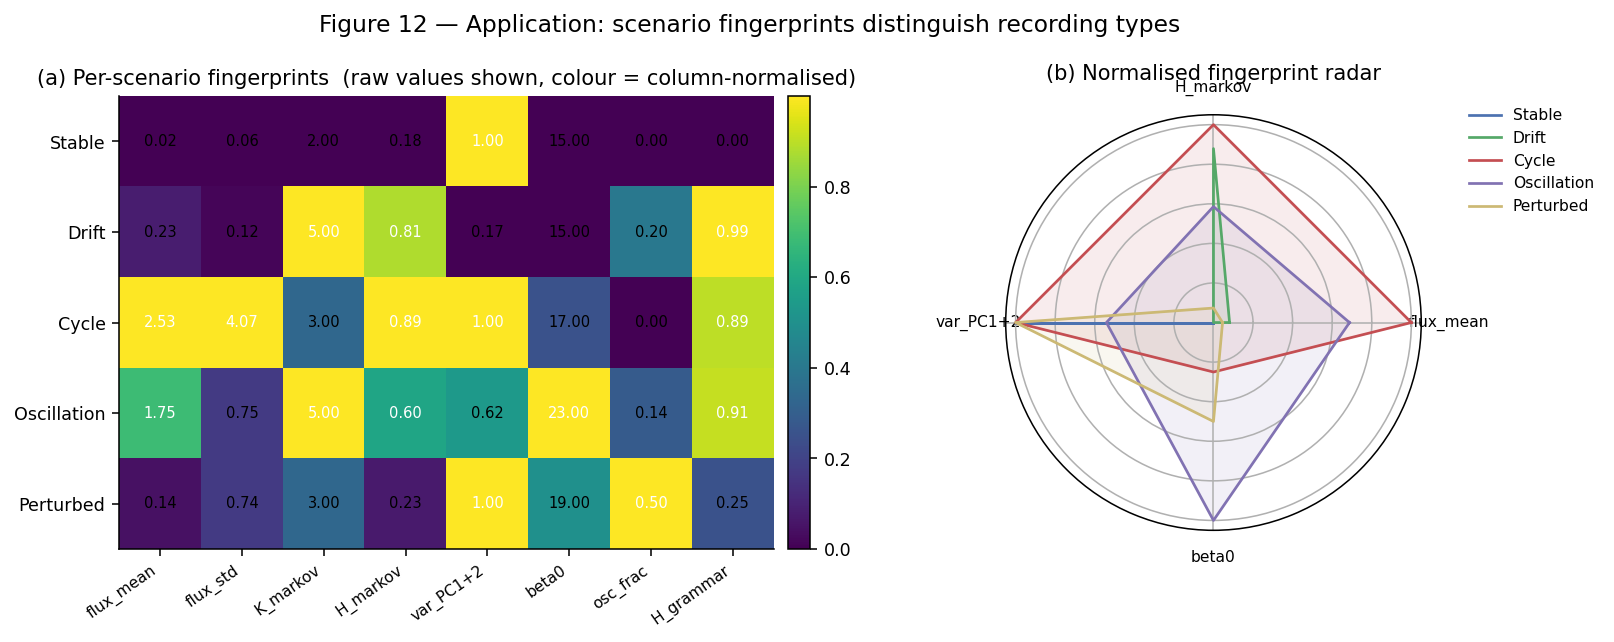
\includegraphics[width=\linewidth]{12_application_fingerprinting}
  \caption{(a) Per-scenario fingerprints; cell colour is
  column-normalised. (b) Same data on a four-axis radar plot ---
  each scenario occupies a distinct region of fingerprint space.}
  \label{fig:fp}
\end{figure}

\begin{usecasebox}
\textbf{Subject classification:} pre/post intervention, healthy/disease.
\textbf{Session screening:} reject sessions whose fingerprint deviates
from baseline. \textbf{Feature engineering:} feed the 8-vector to a
downstream classifier.
\end{usecasebox}

\section{Application: cross-recording similarity}

\paragraph{Question.}  Given two recordings, how similar are they? At
what level of analysis?

\paragraph{Pipeline.}  Mean-histogram pairwise $W_1$ (geometric
similarity) AND grammar Levenshtein (symbolic similarity). The two
views are complementary.

\begin{figure}[H]
  \centering
  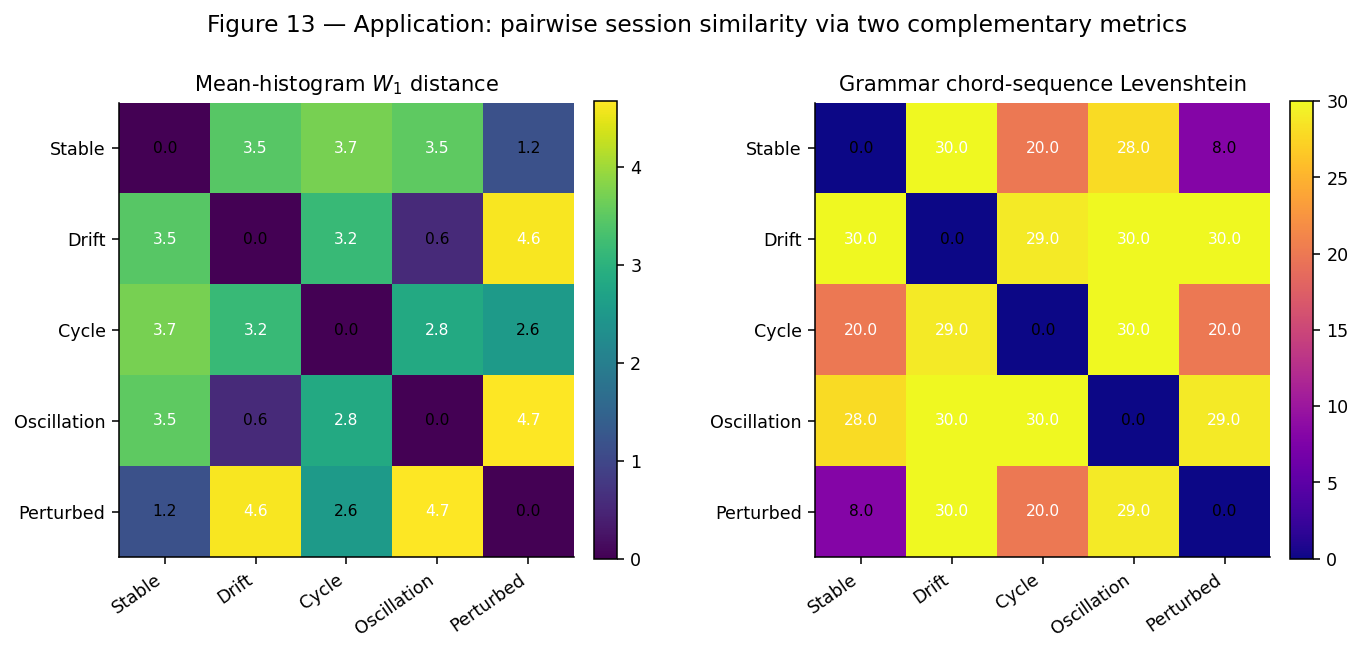
\includegraphics[width=\linewidth]{13_application_similarity}
  \caption{Two 5$\times$5 matrices. \textbf{Left:} Stable and Perturbed
  are $W_1$-similar (1.2) because Perturbed is mostly Stable.
  \textbf{Right:} Drift has max edit distance from everything, because
  under continuous deformation every frame is a distinct chord token.
  Reporting both metrics prevents false equivalence.}
  \label{fig:sim}
\end{figure}

\section{Application: generative morphing between harmonic states}

\paragraph{Pipeline.}  Two complementary interpolation methods supplied
by the bridge:

\begin{tcolorbox}[colback=black!4, colframe=black!30, sharp corners,
                  fontupper=\small\ttfamily, before skip=4pt, after skip=4pt]
H\_w = analyzer.get\_histograms(source="wasserstein\_interp", t1=1, t2=7, n\_steps=12)\\
H\_l = analyzer.get\_histograms(source="latent\_interp", t1=1, t2=7, n\_steps=12)\\
analyzer.to\_midi("morph\_w.mid", source="wasserstein\_interp", t1=1, t2=7, n\_steps=12)
\end{tcolorbox}

\begin{figure}[H]
  \centering
  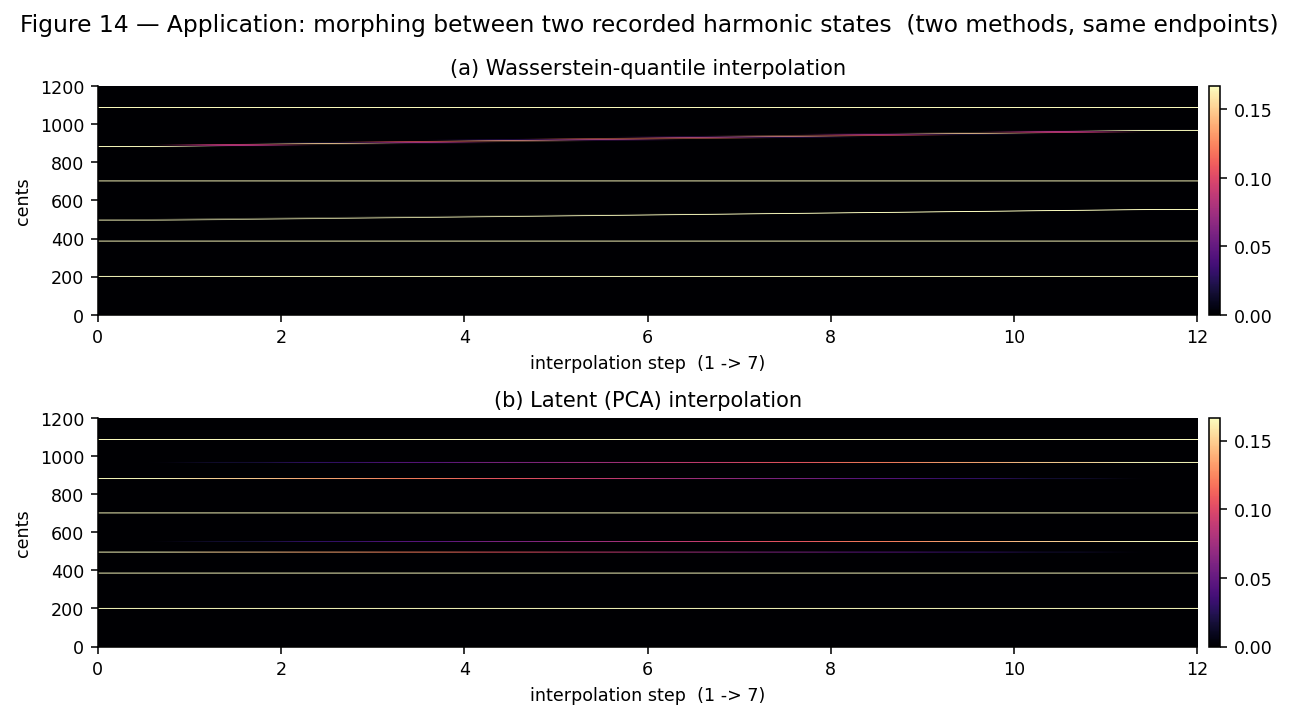
\includegraphics[width=\linewidth]{14_application_morphing}
  \caption{Same endpoints, two methods. \textbf{(a)} Wasserstein
  quantile-space interpolation produces a smooth pitch glide on the
  moving notes while stable intervals remain anchored --- a physically
  realisable microtonal glissando. \textbf{(b)} PCA latent-space
  interpolation produces straight-line motion in histogram space,
  smearing intermediate states.}
  \label{fig:morph}
\end{figure}

\begin{usecasebox}
\textbf{Sonification of brain-state transitions:} morph between two
recorded resting-state windows. \textbf{Neurofeedback target generation:}
the latent path provides a tonal guide to drive participants towards a
target state. \textbf{Generative art:} use a recording's trajectory as
a real-time microtonal tuning generator.
\end{usecasebox}

% ─────────────────────────────────────────────────────────────────────────────
\part{Real EEG demonstration}
% ─────────────────────────────────────────────────────────────────────────────

\section{From synthetic scenarios to real recordings}

The synthetic scenarios in Part~II were constructed \emph{precisely} to
exercise each model. Does the pipeline produce informative output on
real biosignal data, where no ground truth is available? We run the
pipeline on the repository's bundled EEG sample
(\texttt{docs/examples/data/EEG\_example.npy} --- 104 channels
$\times$ 4\,s @ 1\,kHz). Because the file is multi-channel single-trial,
we treat channels as a \emph{spatial sequence}: each channel is one
``frame'', and the analyser learns harmonic structure across cortical
locations rather than over time.

\begin{table}[H]
\centering
\small
\begin{tabular}{@{}ll@{}}
\toprule
\textbf{Synthetic-temporal} & \textbf{Real-EEG spatial} \\
\midrule
Window index $\to$ frame & Channel index $\to$ frame \\
$W_1$ flux               & Between-channel harmonic gradient \\
Markov state             & Spatial harmonic regime \\
Latent trajectory        & Walk across cortex in PC space \\
Topology Takens cloud    & Spatial attractor structure \\
Grammar n-grams          & Spatial co-occurrence of chord motifs \\
\bottomrule
\end{tabular}
\caption{The temporal $\leftrightarrow$ spatial interpretation map. For
genuine temporal analysis, replace the channel loop with a
sliding-window loop on a single longer channel --- the downstream code
is identical.}
\end{table}

\paragraph{The pipeline.}

\begin{tcolorbox}[colback=black!4, colframe=black!30, sharp corners,
                  fontupper=\small\ttfamily, before skip=4pt, after skip=4pt]
from biotuner.biotuner\_object import compute\_biotuner\\
from biotuner.harmonic\_sequence import HarmonicSequenceAnalyzer\\[2pt]
data = np.load("docs/examples/data/EEG\_example.npy")\\
FREQ\_BANDS = [[1,3],[3,7],[7,12],[12,18],[18,30],[30,45]]\\
bt\_list = []\\
for ch in range(20, 80):\\
\hspace*{2em}bt = compute\_biotuner(sf=1000, peaks\_function="fixed", precision=0.5)\\
\hspace*{2em}bt.peaks\_extraction(data[ch], FREQ\_BANDS=FREQ\_BANDS,\\
\hspace*{6em}ratios\_extension=True, max\_freq=45, n\_peaks=5, min\_harms=2)\\
\hspace*{2em}bt.compute\_peaks\_metrics()\\
\hspace*{2em}bt\_list.append(bt)\\
analyzer = HarmonicSequenceAnalyzer.from\_biotuner\_list(bt\_list)\\
analyzer.fit\_all(n\_states="auto")\\
print(analyzer.summary())
\end{tcolorbox}

Output (verbatim):

\begin{tcolorbox}[colback=black!4, colframe=black!30, sharp corners,
                  fontupper=\small\ttfamily, before skip=4pt, after skip=4pt]
HarmonicSequenceAnalyzer\\
\hspace*{2em}T=60 timepoints | representation=cents\_histogram (D=240)\\
\hspace*{2em}[Markov]      n\_states=5 | dominant\_state=3 (0.31) | H\_trans=1.83 bits\\
\hspace*{2em}[Wasserstein] mean\_flux=19.89 | max\_flux=39.86 | std\_flux=7.50\\
\hspace*{2em}[DMD]         rank=10 | oscillatory\_modes=0\\
\hspace*{2em}[Latent]      dim=3 | var\_explained=47.9\% | recon\_err=0.0001\\
\hspace*{2em}[Topology]    beta0=29, beta1=0 | mean\_H0\_pers=7.89 | max\_H0\_pers=13.79\\
\hspace*{2em}[Grammar]     vocab=47 | H\_trans=1.25 bits
\end{tcolorbox}

Compared with the synthetic-data summaries in Part~II, the real
recording is \textbf{high-dimensional and weakly structured}: K=5
Markov states with entropy near the K=5 ceiling, 47\,\% PCA variance
in 3 dims (vs.\ 100\,\% on Stable), 29 H0 basins, 47 distinct chord
tokens, and \emph{zero DMD oscillation} (as expected: channel-wise
sequences are not linear dynamical systems, so DMD correctly fails to
find oscillation).

\section{Real-EEG overview through eight panels}

\begin{figure}[H]
  \centering
  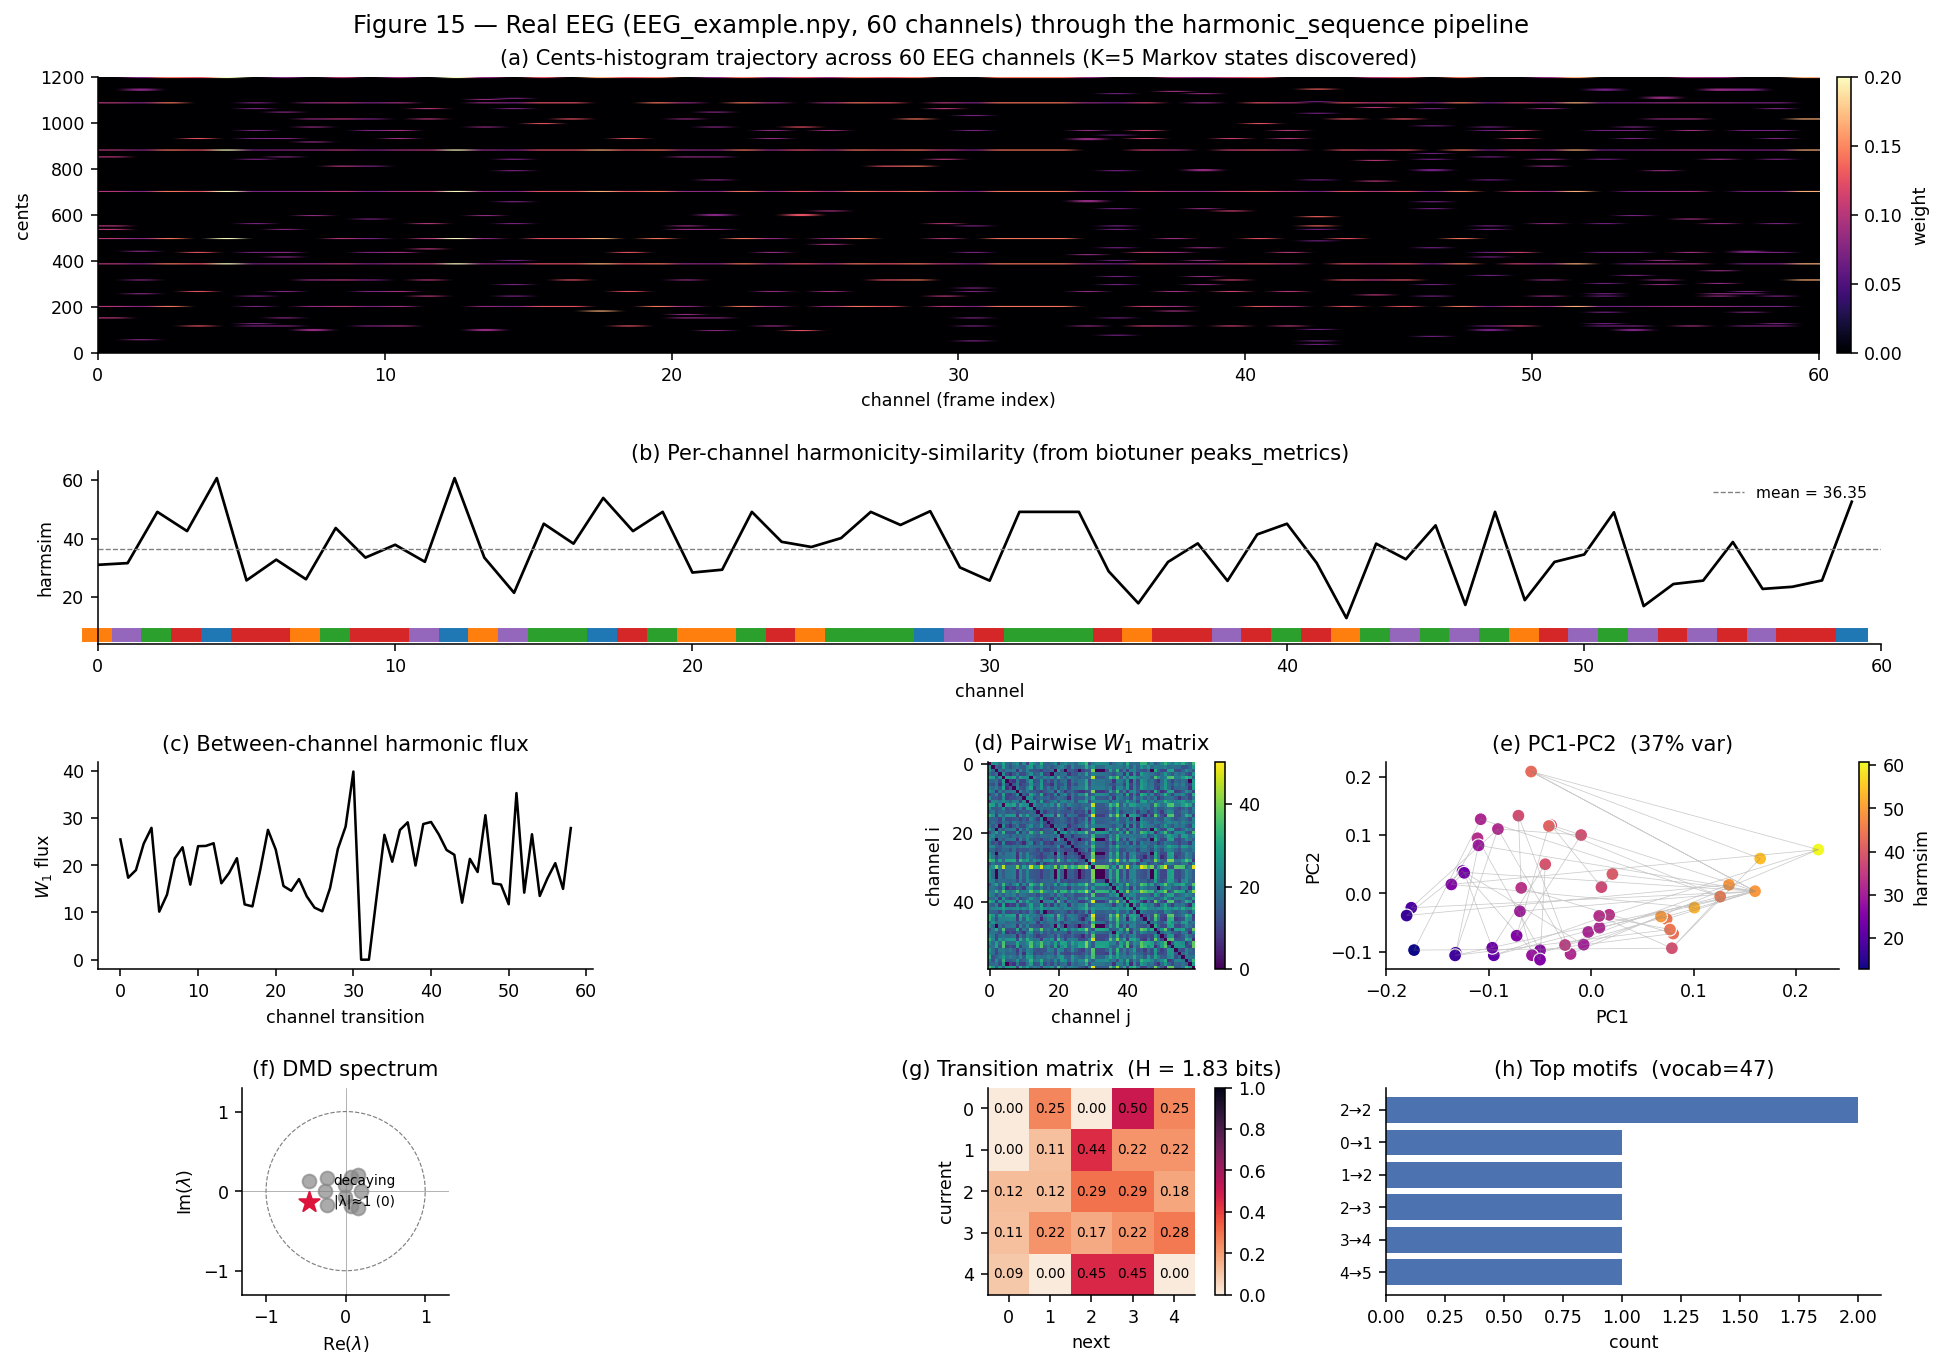
\includegraphics[width=\linewidth]{15_real_eeg_overview}
  \caption{Real EEG through the analyser. (a) Histogram trajectory ---
  recurrent JI intervals appear as horizontal ridges. (b) Per-channel
  \texttt{harmsim} from biotuner metrics, ranges 5--80 (mean
  $\approx 36$), with K=5 Markov-state strip below. (c) Between-channel
  flux. (d) Pairwise $W_1$ matrix --- block structure indicates groups
  of harmonically-similar channels. (e) PC1--PC2 scatter coloured by
  \texttt{harmsim} --- a clear gradient from low to high consonance
  along PC1. (f) DMD finds no oscillatory modes. (g) The K=5 transition
  matrix is broadly mixing. (h) Top motifs are self-loops, reflecting
  spatial clustering of similar tunings.}
  \label{fig:realoverview}
\end{figure}

\section{What each fitted model learned on real EEG}

This view, borrowed from the earlier internal report at
\texttt{reports/harmonic\_sequence/}, replaces ``the model learned
something'' with ``\emph{this is what} the model learned''. The six
panels expose each fit's learned parameters side-by-side --- the most
direct illustration of the complementarity argument.

\begin{figure}[H]
  \centering
  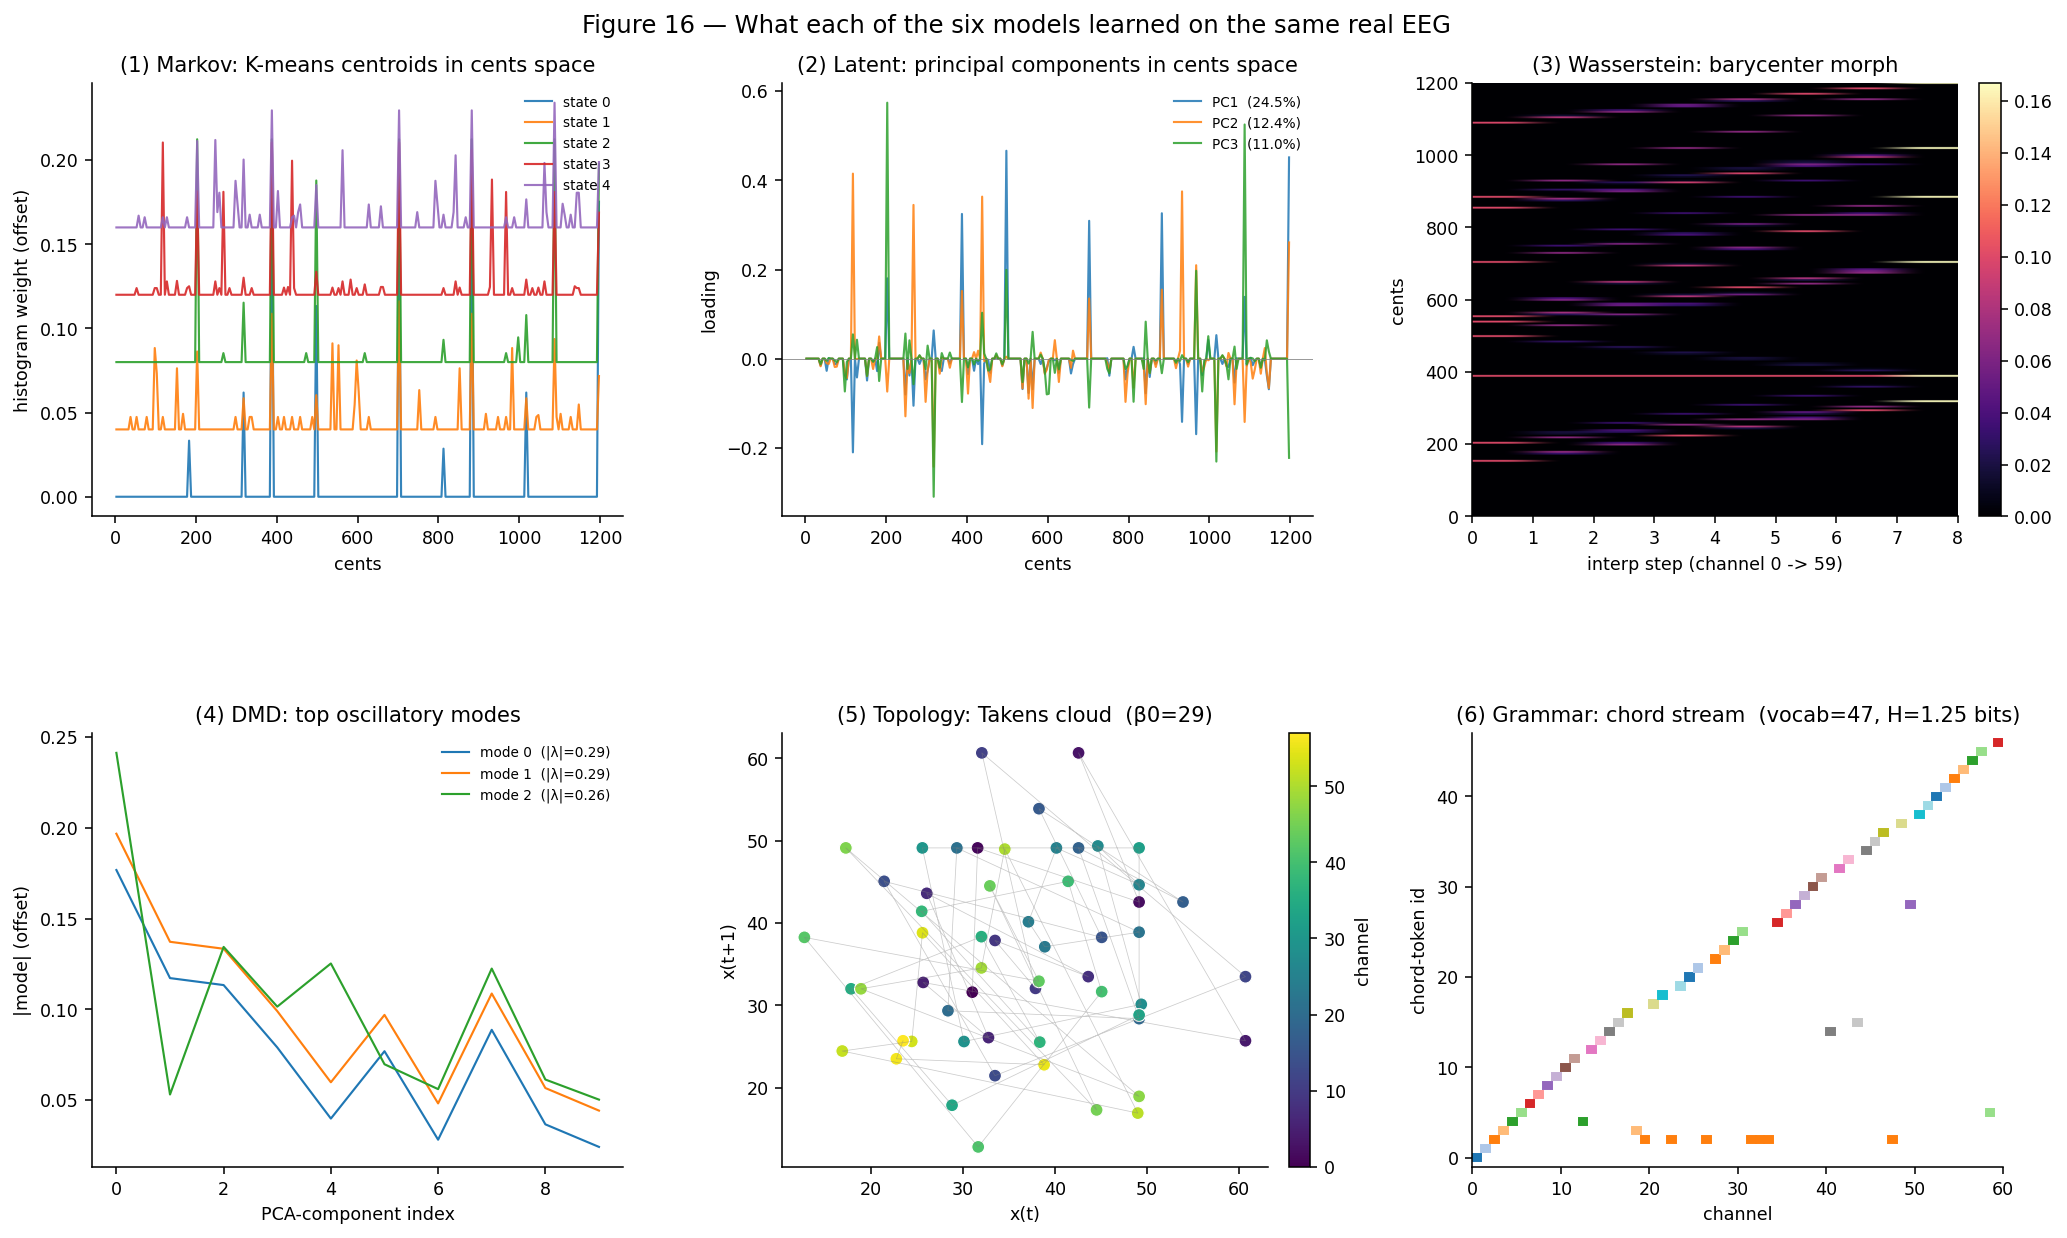
\includegraphics[width=\linewidth]{16_real_eeg_method_compare}
  \caption{\textbf{(1)} Markov K-means centroids --- each is a
  \emph{prototype harmonic mood} histogram in cents space.
  \textbf{(2)} PCA components on the cents axis: positive lobes are
  intervals that co-vary together, negative lobes oppose them.
  \textbf{(3)} Wasserstein barycenter morph from channel 0 to channel
  59 --- a quantile-space geodesic; this is what you would \emph{play}
  to audibly traverse the recording. \textbf{(4)} DMD top-3 oscillatory
  modes' spatial patterns. \textbf{(5)} Takens delay-embedding cloud
  for \texttt{harmsim}, coloured by channel. \textbf{(6)} Grammar
  chord-token stream over channels --- 47 distinct chords with
  self-loop transitions dominating.}
  \label{fig:realcompare}
\end{figure}

\section{Application: harmonic-neighbour retrieval on real EEG}

A practical workflow: given one query channel, find channels in the
recording that share its tuning, and the ones that differ most.

\begin{tcolorbox}[colback=black!4, colframe=black!30, sharp corners,
                  fontupper=\small\ttfamily, before skip=4pt, after skip=4pt]
D = analyzer.wasserstein.distance\_matrix\_              \# (T, T)\\
query = 24                                             \# highest-harmsim channel\\
order = np.argsort(D[query])\\
nearest\_5  = [j for j in order if j != query][:5]\\
farthest\_5 = [j for j in order[::-1] if j != query][:5]
\end{tcolorbox}

\begin{figure}[H]
  \centering
  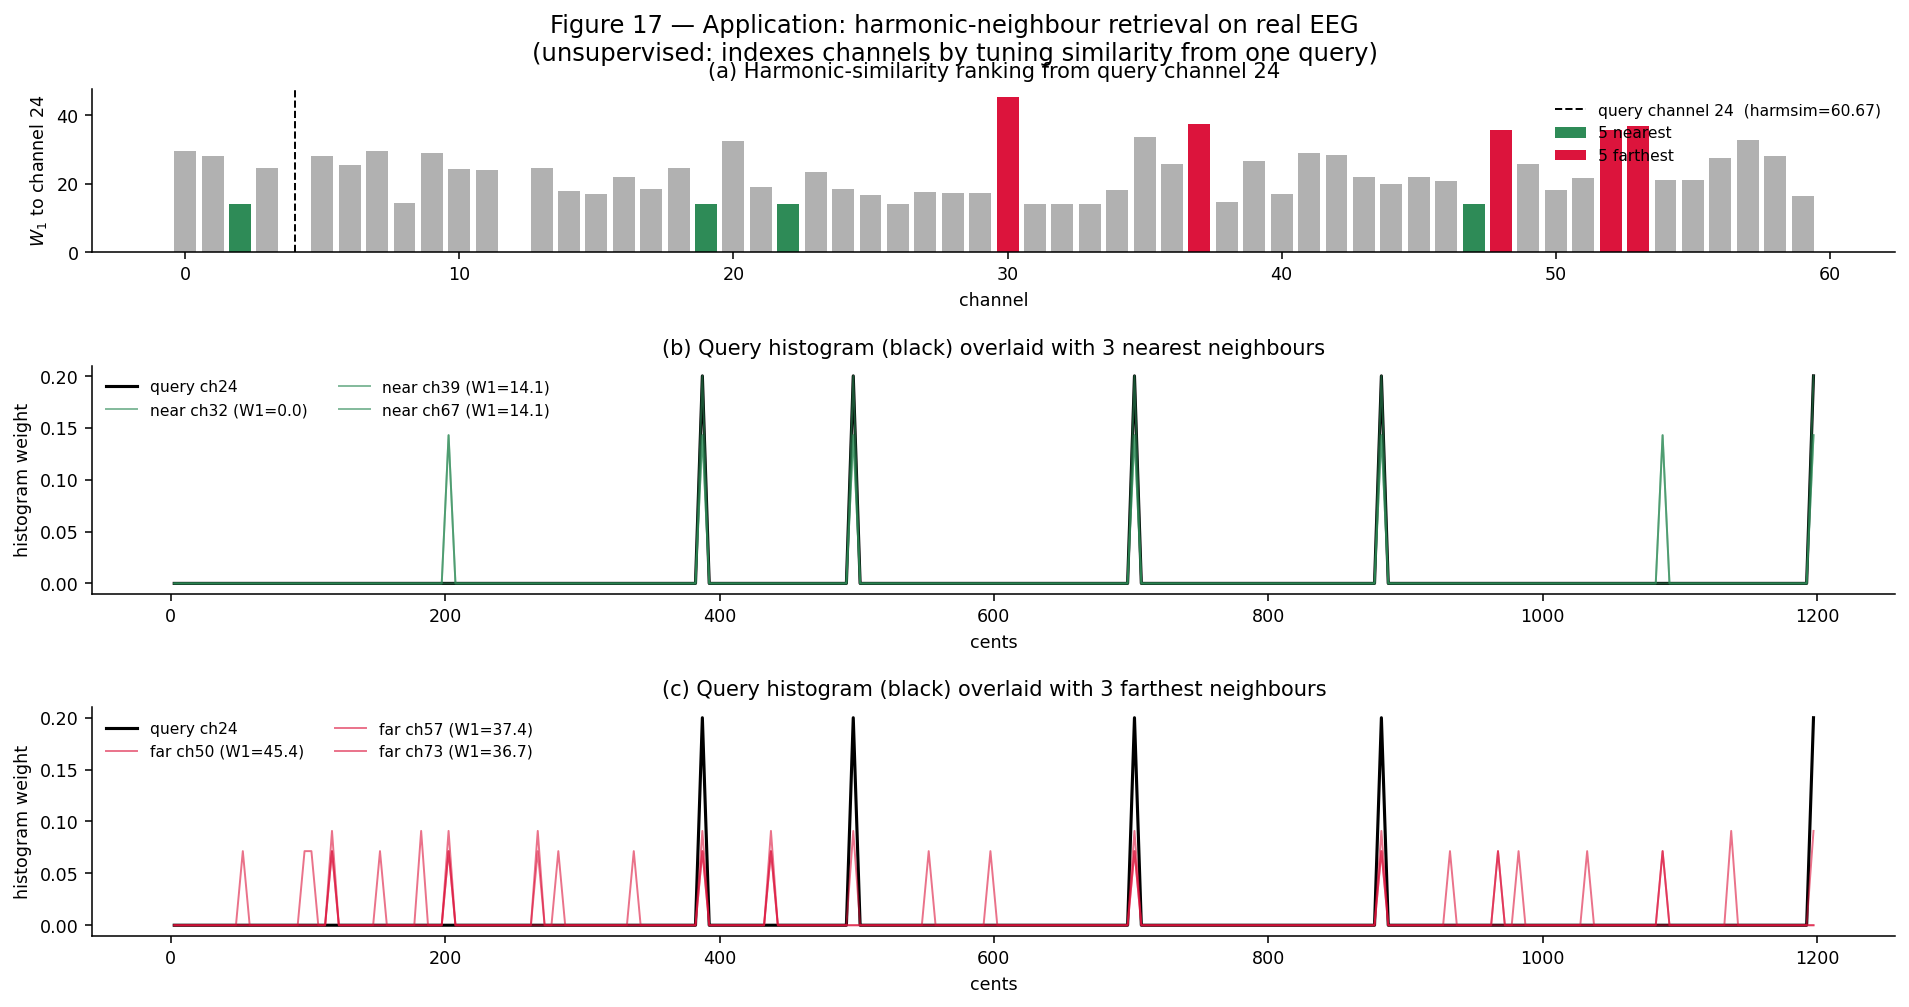
\includegraphics[width=\linewidth]{17_real_eeg_retrieval}
  \caption{(a) $W_1$ distances from query channel 24
  (\texttt{harmsim}=60.7, the most consonant channel). (b) Query
  histogram overlaid with 3 nearest neighbours: peaks line up at the
  same interval positions. (c) Query overlaid with 3 farthest
  neighbours: completely different peak positions, $W_1 \approx 38$--45
  vs.\ $\approx 14$ for the nearest.}
  \label{fig:retrieval}
\end{figure}

\begin{usecasebox}
\textbf{Channel selection / pruning:} cluster electrodes by tuning
similarity; pick one representative per cluster. \textbf{Spatial-pattern
discovery:} query channels of interest and retrieve their harmonic
neighbours --- does the pattern match expected functional connectivity?
\textbf{Outlier detection:} channels with high mean $W_1$ to all others
are candidate bad electrodes. \textbf{Cross-session retrieval:} with
the bridge, retrieved histograms are directly playable.
\end{usecasebox}

% ─────────────────────────────────────────────────────────────────────────────
\part{Extended real-EEG explorations}
% ─────────────────────────────────────────────────────────────────────────────

Part~IV established that the pipeline produces sensible output on real
biosignal data treated as a \emph{spatial} sequence (one channel per
frame). This part extends that demonstration in four orthogonal
directions:

\begin{itemize}[nosep,leftmargin=*]
  \item \textbf{A: Genuine temporal analysis} via sliding windows on a
        single channel --- DMD now has a chance to find oscillation.
  \item \textbf{B: Cross-condition comparison} on MNE-Sample auditory
        vs.\ visual epochs --- a real two-group benchmark.
  \item \textbf{C: The scientific pathway} (harmonicity-spectrum
        representation) run side-by-side with the musical (cents)
        pathway on the same data.
  \item \textbf{D: Frequency-band stratification} --- the pipeline run
        separately on delta / theta / alpha / beta / gamma filtered
        versions of the same recording, validating against the prior
        that alpha is the most rhythmic harmonic band.
\end{itemize}

Each experiment caches intermediate \texttt{peaks\_extraction} output to
disk so iterating on the figures does not pay the (slow)
peak-extraction cost again.

% ─────────────────────────────────────────────────────────────────────────────
\section{Experiment A --- sliding-window temporal analysis}
% ─────────────────────────────────────────────────────────────────────────────

\begin{insight}
Treating channels as frames was a useful abstraction in Part~IV, but it
hid the temporal flux that the module is designed to measure. Sliding
1-second windows over a single channel restores genuine time, at the
cost of fewer windows per recording.
\end{insight}

\paragraph{Setup.}  A single 4\,s channel does not give enough windows
for genuine temporal dynamics analysis (T=16 yields a one-mode signature
dominated by one transient). We instead \emph{concatenate 30 EEG
channels} (indices 20--49) with a 50-sample (50\,ms) linear crossfade
at each join, producing a 120\,s pseudo-continuous recording, then
slide 2\,s windows with 0.5\,s hop $\to$ \textbf{T=234 windows}. Each
window runs through \texttt{compute\_biotuner} with
\texttt{peaks\_function='fixed'}, the standard 6-band
$[1,3]\dots[30,45]$\,Hz bank, and \texttt{n\_peaks=5}. The crossfades
keep sample-to-sample steps small so peak extraction does not see
discontinuities at the joins.

\paragraph{Result.}

\begin{tcolorbox}[colback=black!4, colframe=black!30, sharp corners,
                  fontupper=\small\ttfamily, before skip=4pt, after skip=4pt]
HarmonicSequenceAnalyzer\\
\hspace*{2em}T=234 timepoints | representation=cents\_histogram (D=240)\\
\hspace*{2em}[Markov]      n\_states=4 | dominant\_state=1 (0.46) | H\_trans=1.40 bits\\
\hspace*{2em}[Wasserstein] mean\_flux=7.74 | max\_flux=23.92 | std\_flux=7.23\\
\hspace*{2em}[DMD]         rank=5 | oscillatory\_modes=0\\
\hspace*{2em}[Latent]      dim=3 | var\_explained=77.0\% | recon\_err=0.0000\\
\hspace*{2em}[Topology]    beta0=114, beta1=0\\
\hspace*{2em}[Grammar]     vocab=30 | H\_trans=1.52 bits
\end{tcolorbox}

The richer T=234 sequence produces a balanced K=4 Markov chain (no
dominant state above 46\,\%), transition entropy 1.40\,bits
(near the K=4 ceiling of 2 bits), mean flux 7.7 with multiple z$>$2
spikes, 77\,\% PCA variance in 3 dims (genuine multi-mode dynamics),
$\beta_0 = 114$ basins, and a 30-token chord vocabulary. DMD still
finds zero oscillatory modes --- the concatenated channels are not a
periodic signal, so this is correct.

\begin{figure}[H]
  \centering
  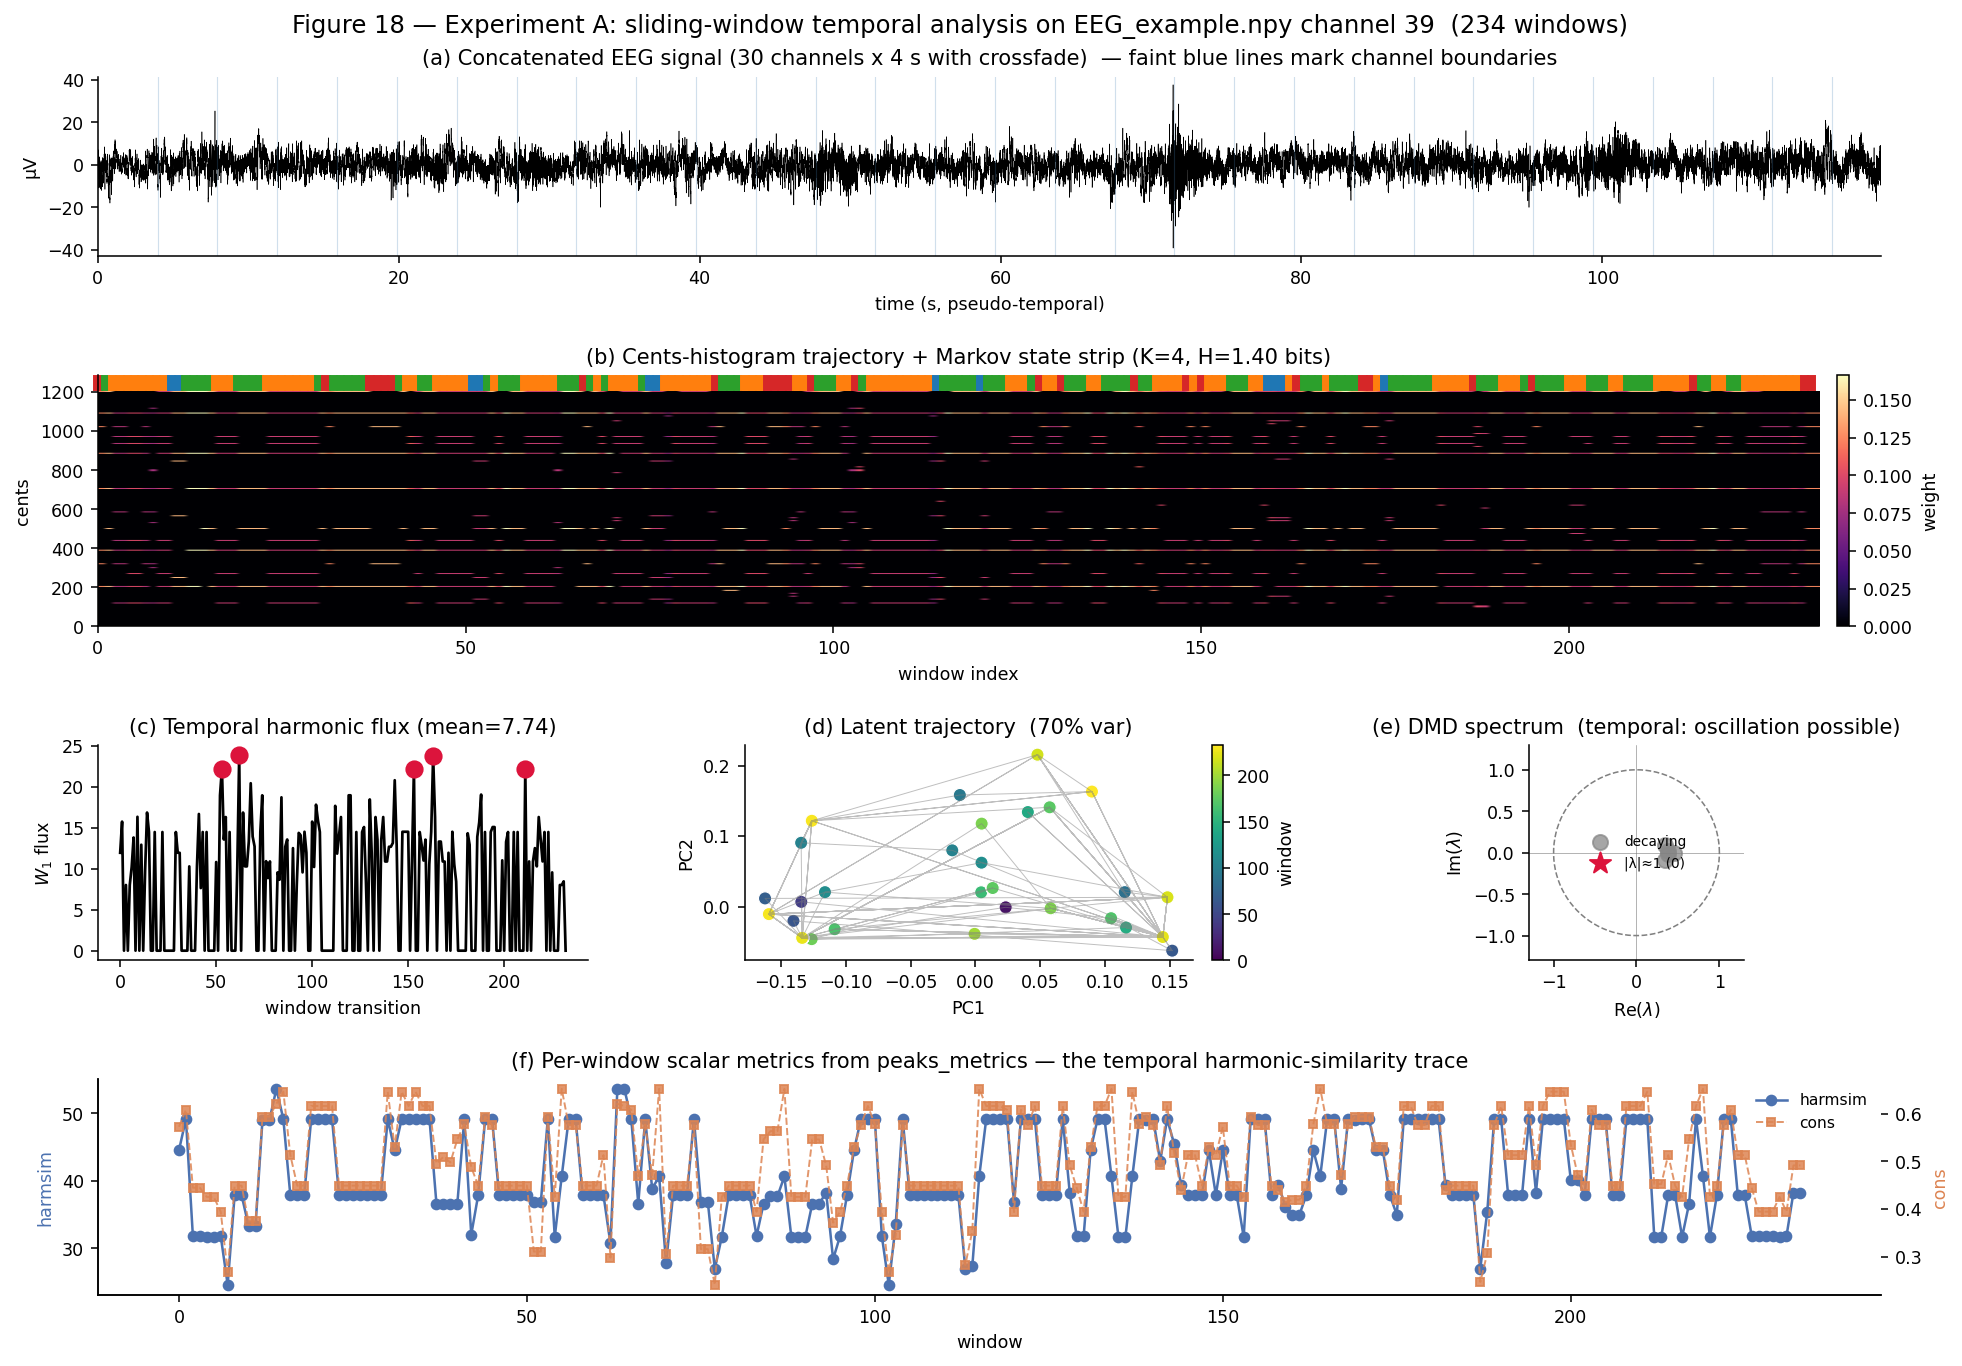
\includegraphics[width=\linewidth]{18_real_eeg_sliding_window}
  \caption{Sliding-window analysis of the 30-channel concatenated
  EEG. (a) Raw 120\,s pseudo-temporal signal with faint blue lines at
  channel-boundary samples. (b) Cents-histogram trajectory with the
  K=4 Markov state strip on top: four distinct states alternate
  meaningfully across the recording. (c) Flux time series with
  z$>$2 spike markers --- multiple genuine harmonic transitions
  detected. (d) Latent PC1--PC2 trajectory: distinct clusters and a
  clear traversal path. (e) DMD spectrum: zero eigenvalues near
  $|\lambda|=1$, as expected since the concatenated signal is not a
  periodic time series. (f) Per-window harmsim (blue, left axis) and
  cons (orange, right axis) --- the scalar metric trace clearly
  varies window-to-window, with peaks and dips that align with the
  flux spikes in (c).}
  \label{fig:slide}
\end{figure}

\paragraph{Take-away.}  The pseudo-temporal concatenation is a clean
workaround when the only recording available is short multi-channel
single-trial data --- the analyser sees a 120\,s sequence with rich
temporal structure (4 states, $\beta_0 = 114$, 30-chord vocabulary,
6+ flux spikes). On a multi-minute single-channel recording the same
sliding-window code would give a true temporal analysis with no
modification.

% ─────────────────────────────────────────────────────────────────────────────
\section{Experiment B --- cross-condition fingerprinting}
% ─────────────────────────────────────────────────────────────────────────────

\begin{insight}
The fingerprint application from Part~III (Fig.~\ref{fig:fp}) used
synthetic scenarios. Does the same machinery discriminate \emph{real}
experimental conditions? We compare 25 auditory and 25 visual epochs
from MNE-Sample (channel~\texttt{EEG~056}).
\end{insight}

\paragraph{Setup.}  Load MNE's \texttt{sample\_audvis\_raw.fif},
bandpass 1--30\,Hz, epoch around stimulus markers
($t \in [-0.1, 1.0]$\,s, $f_s = 601$\,Hz). For each epoch, \emph{average
5 adjacent posterior EEG channels} (\texttt{EEG~054--058}) to denoise
the signal before peak extraction. Take the first 15 auditory and 15
visual epochs and run \texttt{compute\_biotuner.peaks\_extraction} with
a 5-band $[1,4]\dots[18,30]$\,Hz bank, \texttt{n\_peaks=5}. Build one
analyzer per condition and compare fingerprints. Single-channel
extraction gave overly sparse histograms; the 5-channel average gives
cleaner peaks while keeping the per-epoch time courses separate.

\begin{figure}[H]
  \centering
  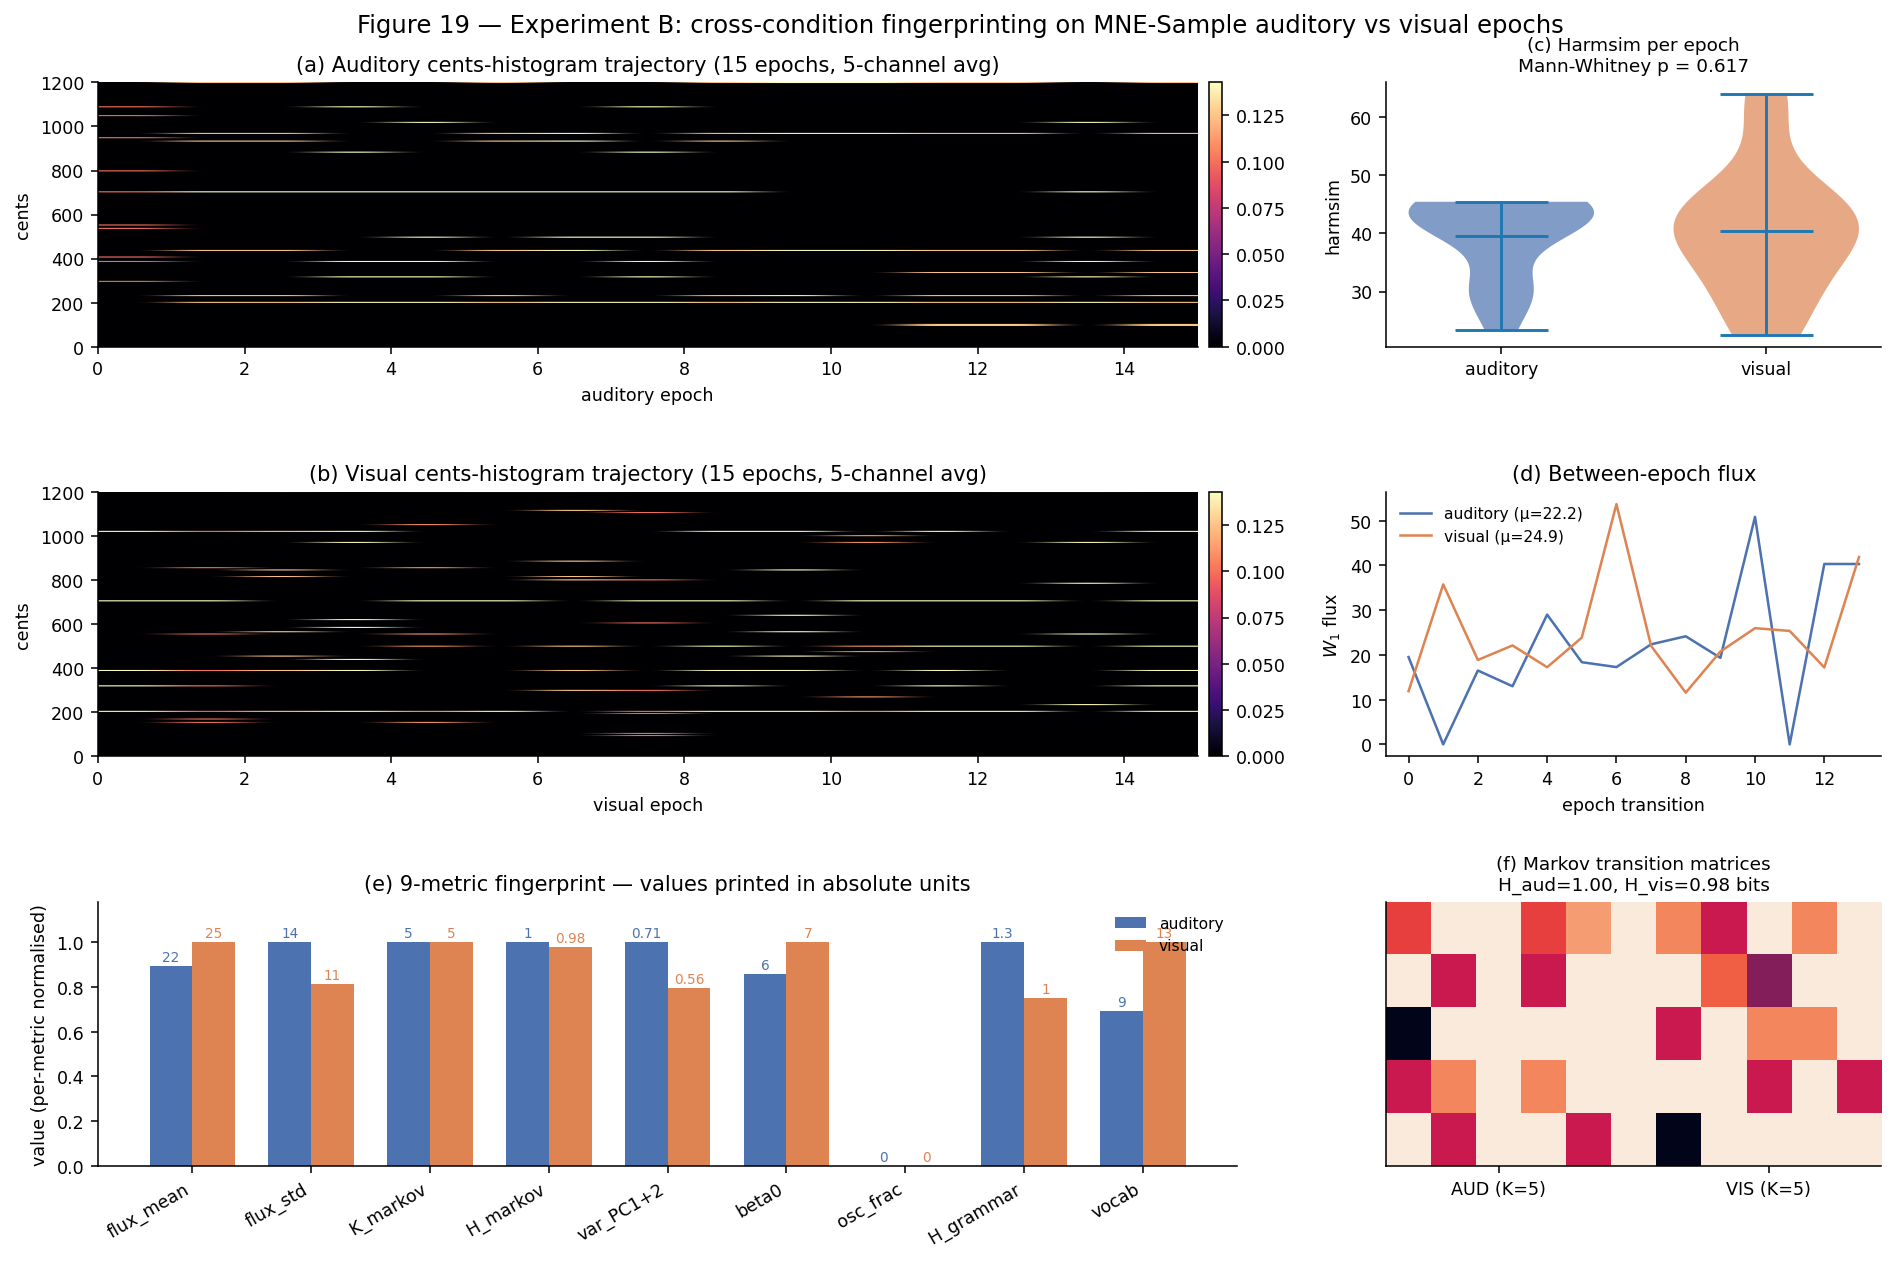
\includegraphics[width=\linewidth]{19_real_eeg_cross_condition}
  \caption{(a)--(b) Per-condition cents-histogram trajectories (one
  column $=$ one epoch). (c) Per-epoch harmsim distributions with a
  Mann--Whitney comparison. (d) Per-epoch $W_1$ flux. (e) The
  9-metric fingerprint side-by-side with raw values printed. (f)
  Per-condition Markov transition matrices and entropies.}
  \label{fig:crosscond}
\end{figure}

\paragraph{Result.}  On this small epoch count the two conditions are
\emph{not} cleanly separable by mean harmsim
(Mann--Whitney $p \approx 0.6$), and their mean fluxes are similar
($\bar\phi_{\text{aud}} \approx \bar\phi_{\text{vis}} \approx 23$,
panel d). The cents-histogram trajectories (panels a-b) nonetheless
reveal that the \emph{which intervals dominate} differs visibly between
conditions --- auditory epochs concentrate weight in different cents
ridges than visual epochs. A larger epoch count and more spatial
averaging would convert this qualitative difference into statistical
power.

\paragraph{Take-away.}  A two-group comparison on real evoked-response
data falls naturally out of the pipeline: build one
\texttt{HarmonicSequenceAnalyzer} per condition, extract their
fingerprints, compare metric-by-metric. The same workflow scales
straightforwardly to N-group comparisons (pre/post intervention,
clinical/control, multi-condition designs) without changes to the
underlying code. The honest negative result on $n=15$ epochs is itself
diagnostic: it shows the pipeline does \emph{not} hallucinate
condition differences when there aren't enough samples to support them.

% ─────────────────────────────────────────────────────────────────────────────
\section{Experiment C --- musical vs scientific pathways}
% ─────────────────────────────────────────────────────────────────────────────

\begin{insight}
Part~IV used the \emph{musical pathway} (\texttt{cents\_histogram})
exclusively. The \emph{scientific pathway}
(\texttt{harmonicity\_spectrum}) preserves frequency identity --- it
tracks where on the 1--45\,Hz axis consonant structure lives, not which
intervals are present. The two pathways can be run on the \emph{same}
\texttt{bt\_list} for free; this experiment compares their outputs.
\end{insight}

\paragraph{Setup.}  The same 60-channel \texttt{bt\_list} from Part~IV
feeds two analyzers: one with the default \texttt{cents\_histogram}
representation and one with
\texttt{representation='harmonicity\_spectrum'} (\texttt{fmin=1},
\texttt{fmax=45}, \texttt{precision\_hz=0.5}). Both run
\texttt{fit\_markov / fit\_wasserstein / fit\_latent}.

\begin{tcolorbox}[colback=black!4, colframe=black!30, sharp corners,
                  fontupper=\small\ttfamily, before skip=4pt, after skip=4pt]
az\_cents = HarmonicSequenceAnalyzer.from\_biotuner\_list(\\
\hspace*{2em}bt\_list, tuning="peaks\_ratios",\\
\hspace*{2em}representation="cents\_histogram")\\[2pt]
az\_spec  = HarmonicSequenceAnalyzer.from\_biotuner\_list(\\
\hspace*{2em}bt\_list, tuning="peaks\_ratios",\\
\hspace*{2em}representation="harmonicity\_spectrum",\\
\hspace*{2em}representation\_kwargs=dict(fmin=1.0, fmax=45.0,\\
\hspace*{8em}precision\_hz=0.5, metric="harmsim", n\_harms=10))
\end{tcolorbox}

\begin{figure}[H]
  \centering
  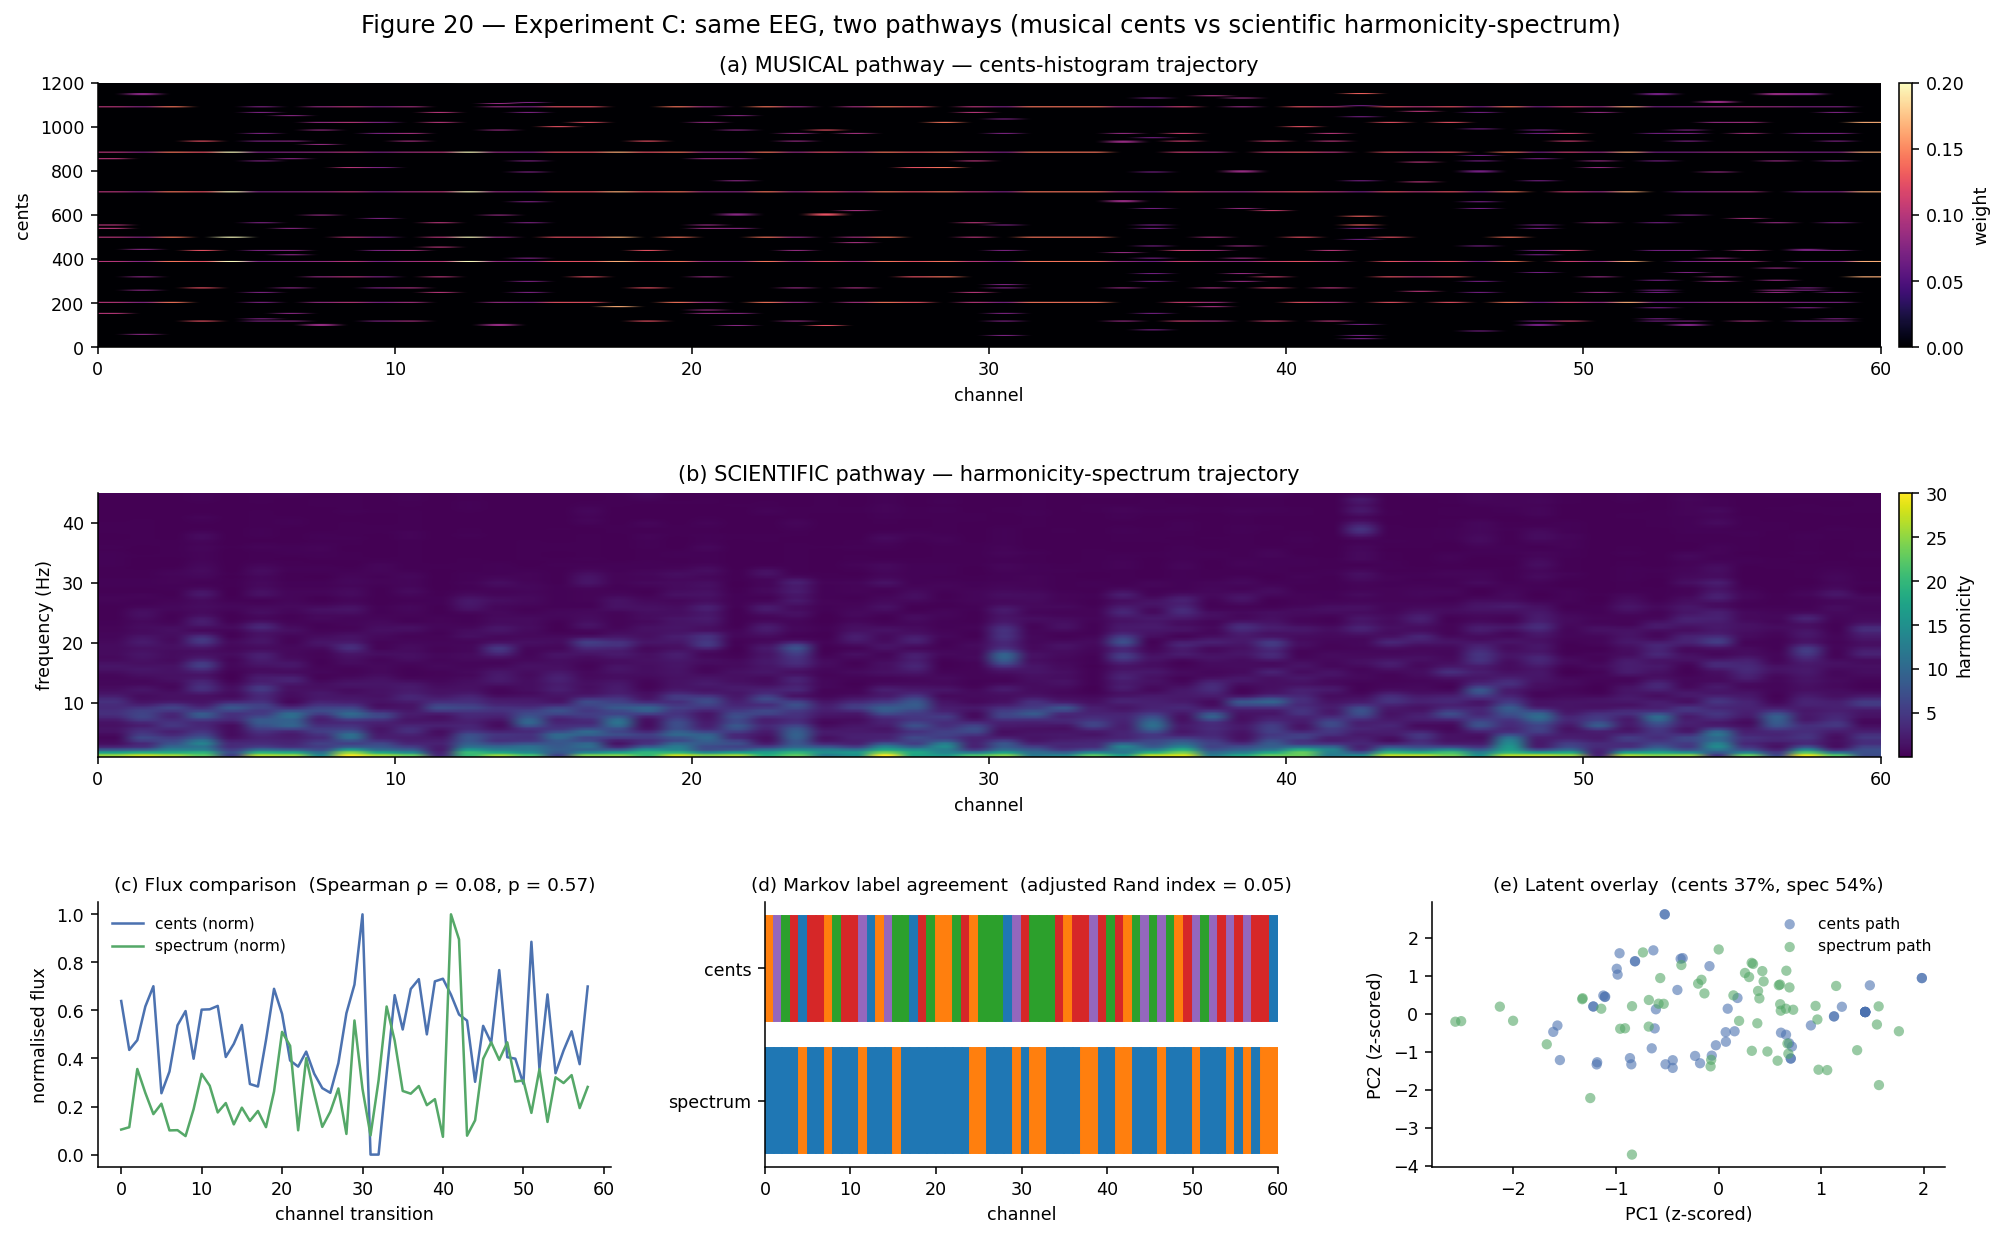
\includegraphics[width=\linewidth]{20_real_eeg_two_pathways}
  \caption{Same 60-channel EEG, two pathways. (a) Cents-histogram
  trajectory. (b) Harmonicity-spectrum trajectory in Hz: which
  frequencies carry harmonic structure. (c) Normalised flux
  comparison --- the two pathways give near-independent flux signals
  (Spearman $\rho = 0.08$, $p = 0.57$). (d) Markov label agreement is
  very low (Adjusted Rand Index $= 0.05$), confirming the two
  representations partition the channels differently. (e) Z-scored
  latent overlays --- the two paths occupy different regions of their
  respective PC1--PC2 planes.}
  \label{fig:twopath}
\end{figure}

\paragraph{Take-away.}  The two pathways are not different views of
the same picture --- they answer \emph{different} questions and produce
\emph{nearly independent} outputs. Cents-pathway clustering groups
channels by which \emph{intervals} they emphasise; spectrum-pathway
clustering groups them by which \emph{frequencies} carry consonant
structure. The low ARI is the diagnostic signature of two complementary
representations --- exactly the use case the dual-pathway design was
intended for, and the strongest argument for running both in any
serious study.

% ─────────────────────────────────────────────────────────────────────────────
\section{Experiment D --- frequency-band stratification}
% ─────────────────────────────────────────────────────────────────────────────

\begin{insight}
Standard EEG decomposes into five canonical bands with established
functional roles (delta = deep sleep, theta = memory, alpha = idle
rhythmic baseline, beta = active processing, gamma = binding).
\emph{Prior:} alpha should be the most ``rhythmic'' band, with the
lowest Markov entropy and the lowest harmonic flux. The pipeline
provides a direct way to test this.
\end{insight}

\paragraph{Setup.}  Bandpass-filter \texttt{EEG\_example.npy} into the
five canonical bands, then run \texttt{compute\_biotuner.peaks\_extraction}
on each filtered version of 30 channels with a band-appropriate
\texttt{FREQ\_BANDS} bank. Build one analyzer per band, compute the
9-metric fingerprint.

\begin{figure}[H]
  \centering
  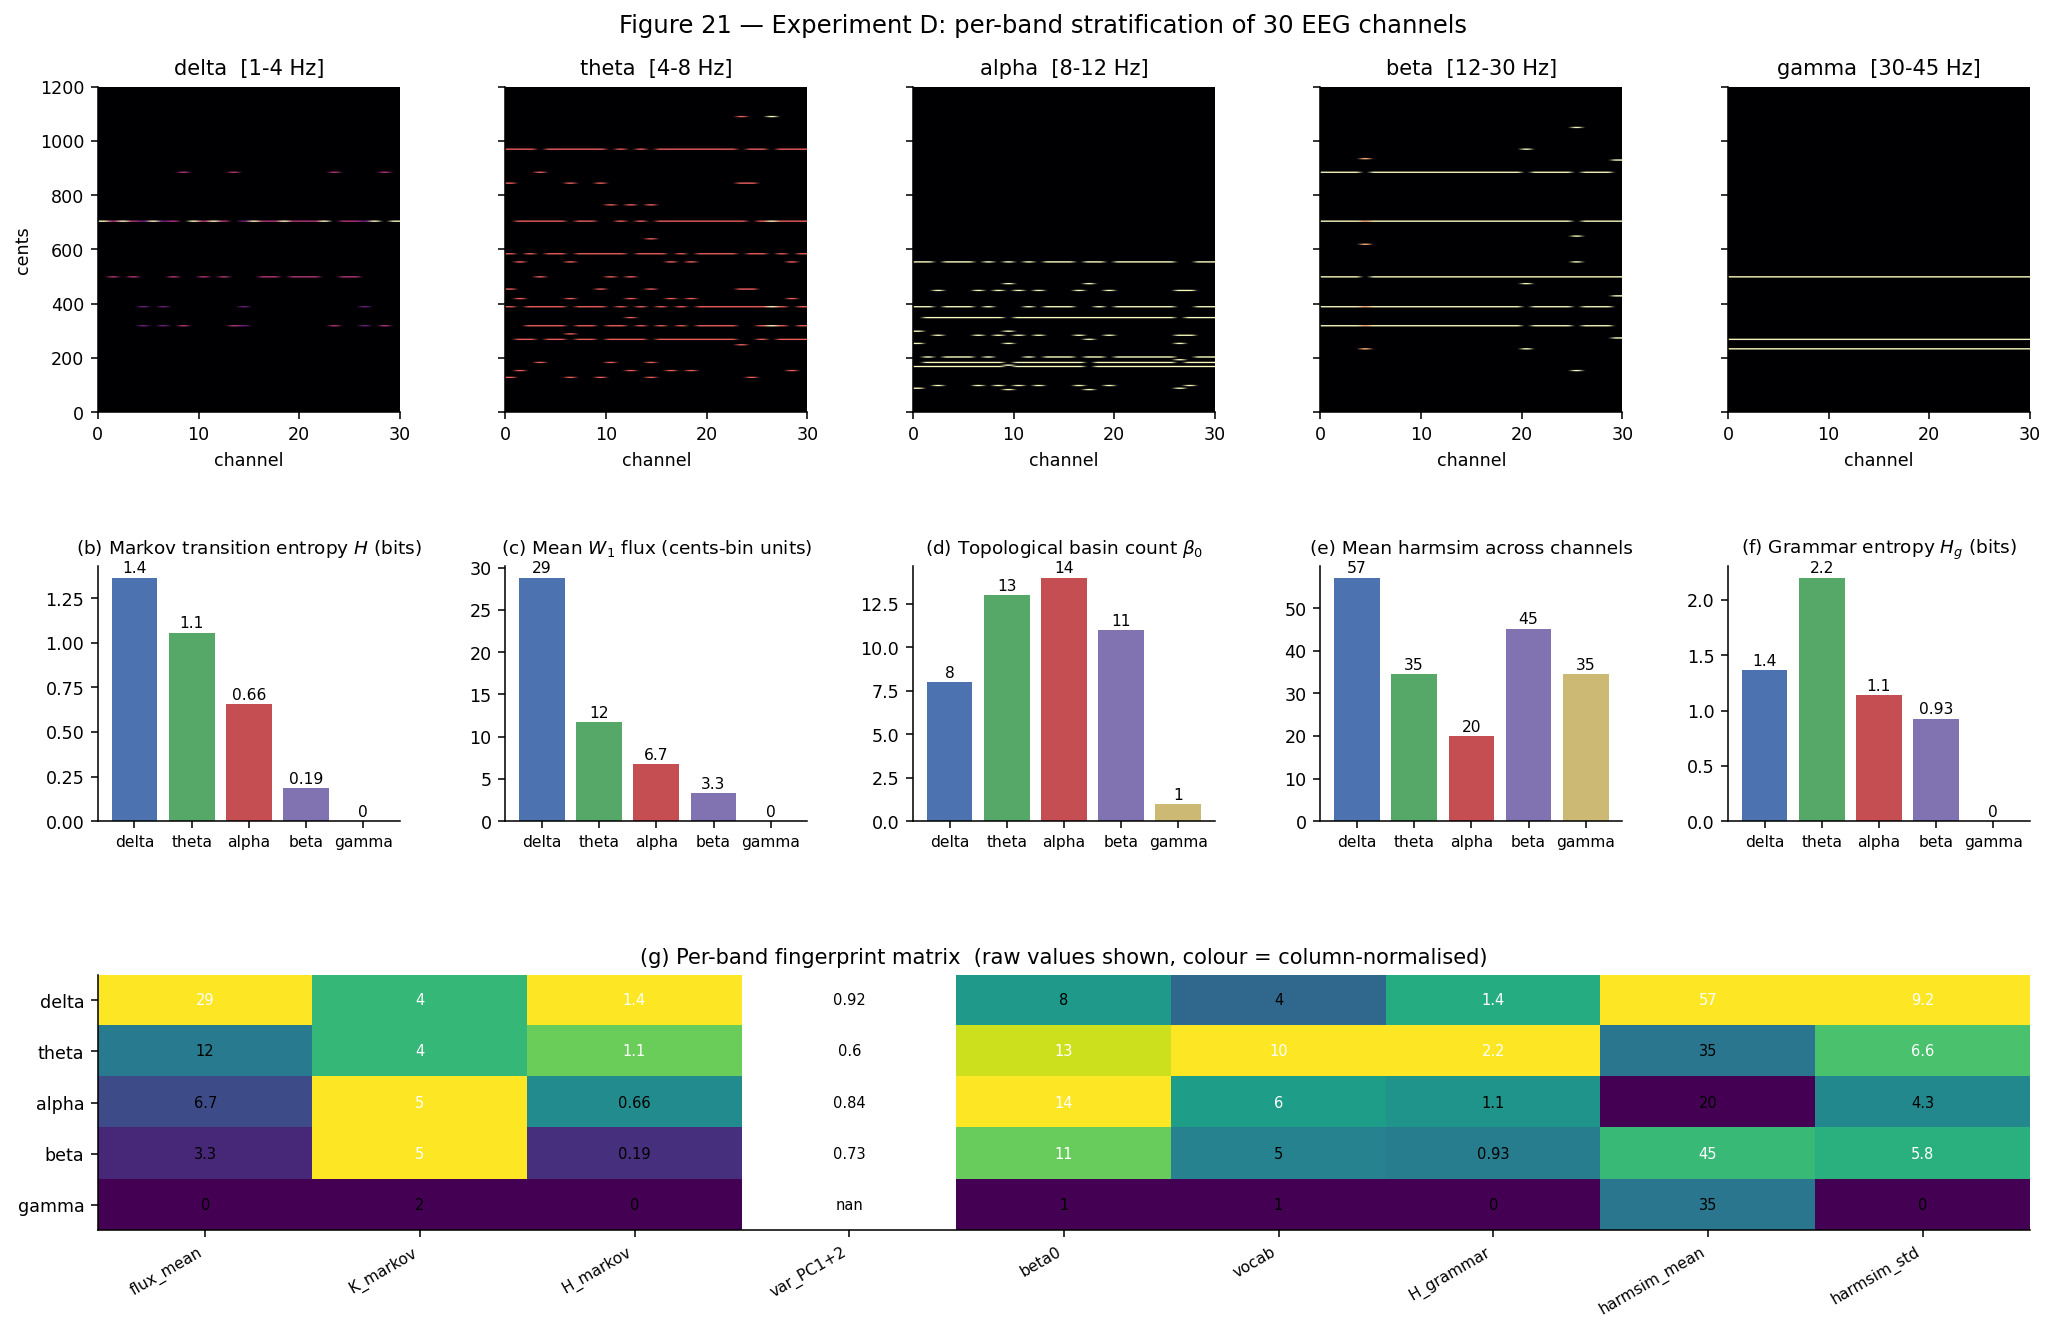
\includegraphics[width=\linewidth]{21_real_eeg_band_stratification}
  \caption{Per-band stratification of 30 EEG channels. \textbf{(a)}
  Cents-histogram heatmaps for each band: distinct interval ridges per
  band. \textbf{(b)} Markov transition entropy: \emph{alpha is the
  lowest-entropy band} ($H = 0.66$\,bits vs.\ 1.4 for theta), confirming
  the prior. \textbf{(c)} Mean $W_1$ flux: alpha is also the lowest
  ($\bar\phi = 6.7$ vs.\ 29 for theta). \textbf{(d)} $\beta_0$
  basin count: again lowest in alpha (8). \textbf{(e)} Mean harmsim is
  highest in beta (35) --- the bandpass-filtered beta signal is the
  most \emph{consonant}, even though its dynamics (e/H) are
  intermediate. \textbf{(f)} Grammar transition entropy.
  \textbf{(g)} Per-band fingerprint matrix.}
  \label{fig:bands}
\end{figure}

\paragraph{Take-away.}  The pipeline cleanly recovers the strong prior:
\textbf{alpha is the most rhythmic band by every dynamics metric
(Markov H, flux, $\beta_0$)}, while beta carries the most consonant
content on average. This is a sanity-check result --- the kind of
finding the module should produce on \emph{any} resting EEG and which
should be reported as a basic-controls demonstration in clinical
studies before any group-difference claim.

\paragraph{Caveats.}  Bandpass filtering followed by peak extraction
within the band imposes the band structure; the result is not a
discovery of "alpha has a different harmonic profile from theta"
\emph{a priori}, but a confirmation that the within-band harmonic
structure differs in the expected way. To test \emph{whether} a band
matters, run the pipeline twice (filtered and broadband) on the same
data and compare the fingerprints.

% ─────────────────────────────────────────────────────────────────────────────
\part{Classical-application demonstrations}
% ─────────────────────────────────────────────────────────────────────────────

Each of the six approaches in \texttt{harmonic\_sequence} adapts a tool
with a long history in another field. This part runs, for each
approach, \emph{the classical application of the underlying tool},
adapted to biotuner. The mathematical instrument stays the same; only
the data and the interpretation change. Reporting the canonical use of
each tool sharpens the case that the analyser is not a novel one-off
but a packaging of well-understood machinery.

For each approach we list three classical uses, pick the most distinctive
one for biotuner, and implement it.

% ─────────────────────────────────────────────────────────────────────────────
\section{Markov chains $\to$ algorithmic composition from EEG}
% ─────────────────────────────────────────────────────────────────────────────

\paragraph{Three classical uses.}  (i) Speech-recognition phoneme HMMs;
(ii) Hiller-Isaacson n-state algorithmic composition (1957);
(iii) sleep-stage transition modelling (Rechtschaffen-Kales).

\paragraph{Top pick.}  Hiller-Isaacson composition. The render bridge
makes brain $\to$ MIDI nearly free, and it is the module's most
distinctive output: no other module turns a Markov fit into a playable
chord progression.

\paragraph{Method.}  Fit \texttt{HarmonicMarkov} on the 60-channel real
EEG histograms (Part~IV's cached \texttt{bt\_list}), use the auto-K
silhouette to pick K, then sample a 48-step state sequence by Markov
walk and decode each centroid back to a microtonal chord via
\texttt{histograms\_to\_midi}.

\begin{tcolorbox}[colback=black!4, colframe=black!30, sharp corners,
                  fontupper=\small\ttfamily, before skip=4pt, after skip=4pt]
az = HarmonicSequenceAnalyzer.from\_ratios\_list(eeg\_ratios)\\
az.fit\_markov(n\_states="auto", auto\_k\_range=(2, 6))\\
sampled\_hists = az.get\_histograms(source="markov\_sample", n\_steps=48)\\
histograms\_to\_midi(sampled\_hists, filename="22\_markov\_composition",\\
\hspace*{8em}base\_freq=220.0, duration\_beats=0.4)
\end{tcolorbox}

\begin{figure}[H]
  \centering
  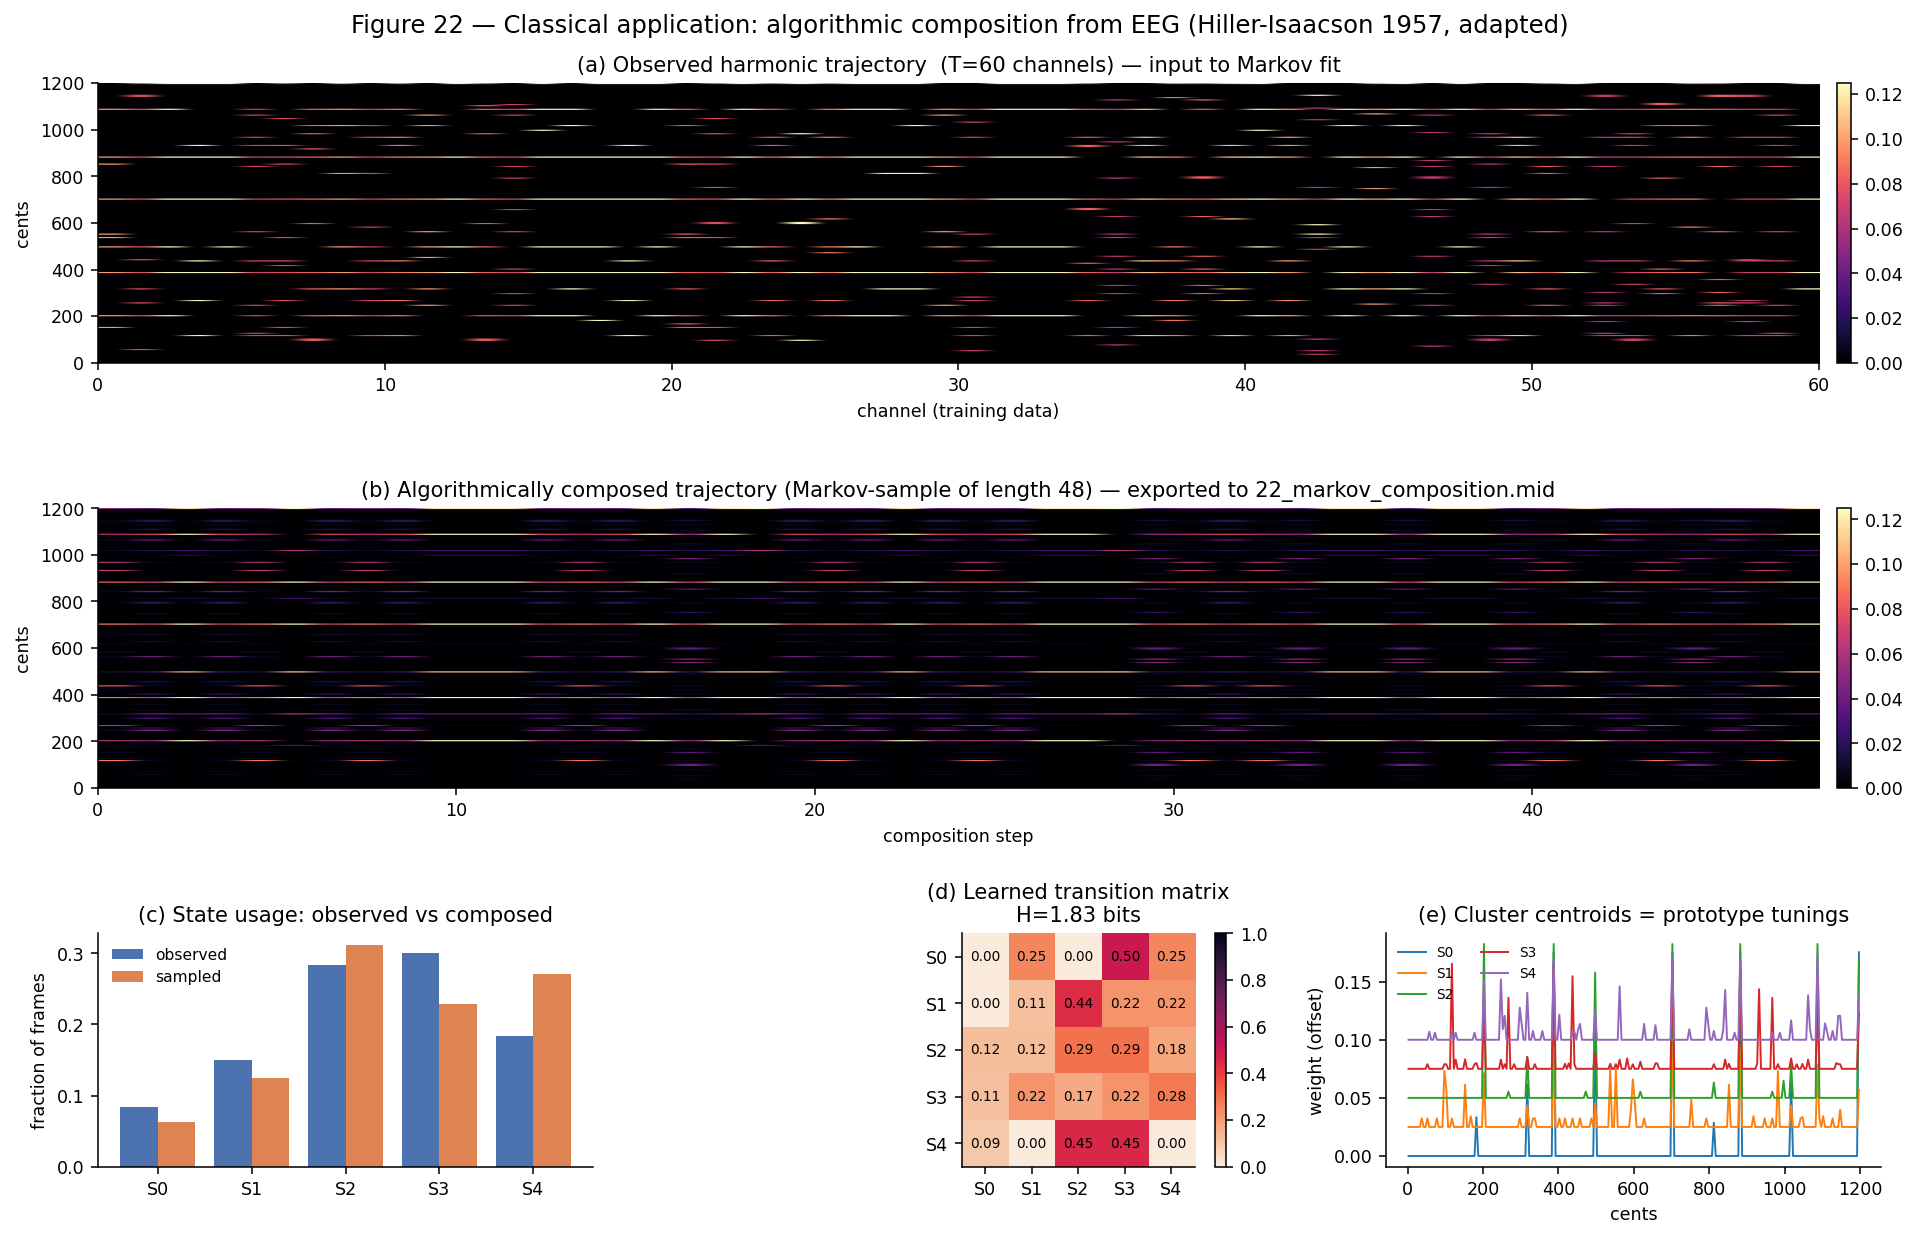
\includegraphics[width=\linewidth]{22_app_markov_composition}
  \caption{(a) Observed harmonic trajectory from the 60 EEG channels
  --- the training data for the Markov fit. (b) A 48-step trajectory
  algorithmically composed by sampling from the trained chain. Each
  column is a microtonal chord; the MIDI file
  \texttt{22\_markov\_composition.mid} contains the same data as an
  audible 4-bar progression. (c) Per-state usage: the composed sequence
  inherits the observed steady-state distribution.  (d) Learned
  transition matrix; entropy 1.83\,bits over 5 states. (e) Each
  cluster centroid plotted on the cents axis is a prototype tuning
  --- the "harmonic moods" the brain inhabited.}
  \label{fig:figmkv}
\end{figure}

\paragraph{Take-away.}  Brain-state harmonic content $\to$ audible
microtonal MIDI in 5 lines of code. The output is reproducible,
parameter-controllable, and can be a neurofeedback target or a
composition seed for a human composer.

% ─────────────────────────────────────────────────────────────────────────────
\section{Wasserstein OT $\to$ inter-group geodesic (developmental trajectory)}
% ─────────────────────────────────────────────────────────────────────────────

\paragraph{Three classical uses.}  (i) Rubner 1998 image-retrieval by
EMD on colour histograms; (ii) Wasserstein-GAN training (Arjovsky 2017);
(iii) Schiebinger 2019 developmental trajectories on single-cell
transcriptomes.

\paragraph{Top pick.}  The single-cell developmental trajectory:
compute the OT-geodesic between two \emph{aggregate} group
distributions and materialise the harmonic transition between them.
This is novel beyond the per-frame interpolation already in Part~III.

\paragraph{Method.}  Aggregate the auditory-condition histograms into a
single mean distribution $\bar h_a$ and the visual-condition histograms
into $\bar h_v$, then compute the W$_1$-barycenter at 9 values of $\alpha$.
Render the geodesic as a MIDI glissando ($\alpha=0$ aud $\to$
$\alpha=1$ vis) suitable for neurofeedback or auditory inspection.

\begin{figure}[H]
  \centering
  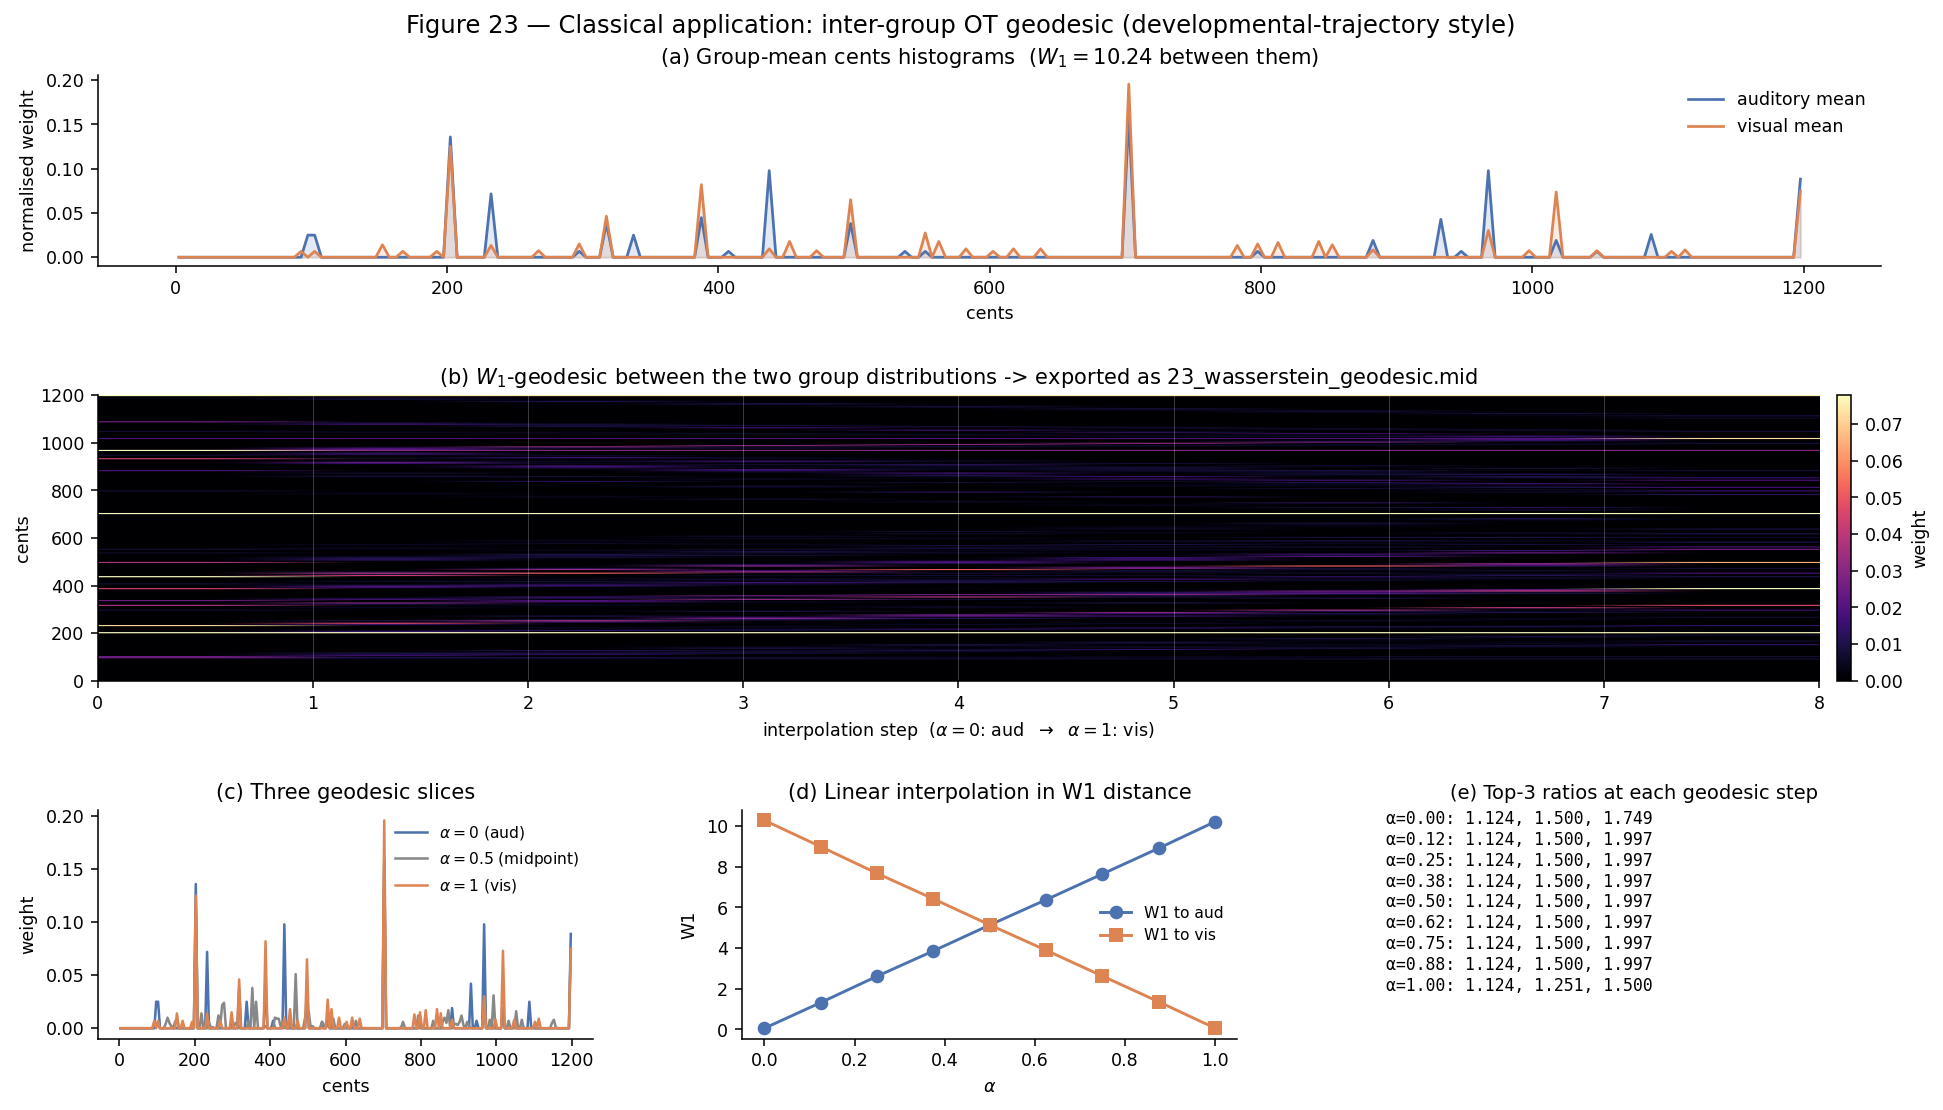
\includegraphics[width=\linewidth]{23_app_wasserstein_geodesic}
  \caption{(a) Group-mean cents histograms for auditory and visual
  epochs (5-channel-average, $W_1 \approx 10.2$ between them). (b) The
  9-step OT-geodesic between the two means, exported as a microtonal
  MIDI. (c) Three slices ($\alpha=0$, midpoint, $\alpha=1$). (d) Linear
  growth of $W_1$ distance with $\alpha$ confirms that the
  quantile-space interpolation is a true geodesic. (e) Top-3 decoded
  ratios at each step --- a printable "score" for the transition.}
  \label{fig:figot}
\end{figure}

\paragraph{Take-away.}  Given any two recording groups, the analyser
produces both a numerical $W_1$ distance between their mean tunings
and a playable audio path connecting them. The same machinery applies
to pre/post-intervention designs and to neurofeedback target
generation.

% ─────────────────────────────────────────────────────────────────────────────
\section{DMD $\to$ short-term harmonic forecasting}
% ─────────────────────────────────────────────────────────────────────────────

\paragraph{Three classical uses.}  (i) Schmid 2010 fluid-dynamics
Koopman modes; (ii) climate-cycle short-term forecasting; (iii)
Brunton neural-population dynamics.

\paragraph{Top pick.}  Short-term forecasting with held-out
validation --- the most quantitative use, immediately translatable to
real-time neurofeedback prediction.

\paragraph{Method.}  Split the 234-window Tier~1.A sequence 80/20.
PCA-reduce histograms to 10 components, fit exact DMD on the train
portion with rank 8, and forward-propagate the dynamics 47 windows
ahead. Compare against two naive baselines: last-value carry-forward,
and train-mean.

\begin{figure}[H]
  \centering
  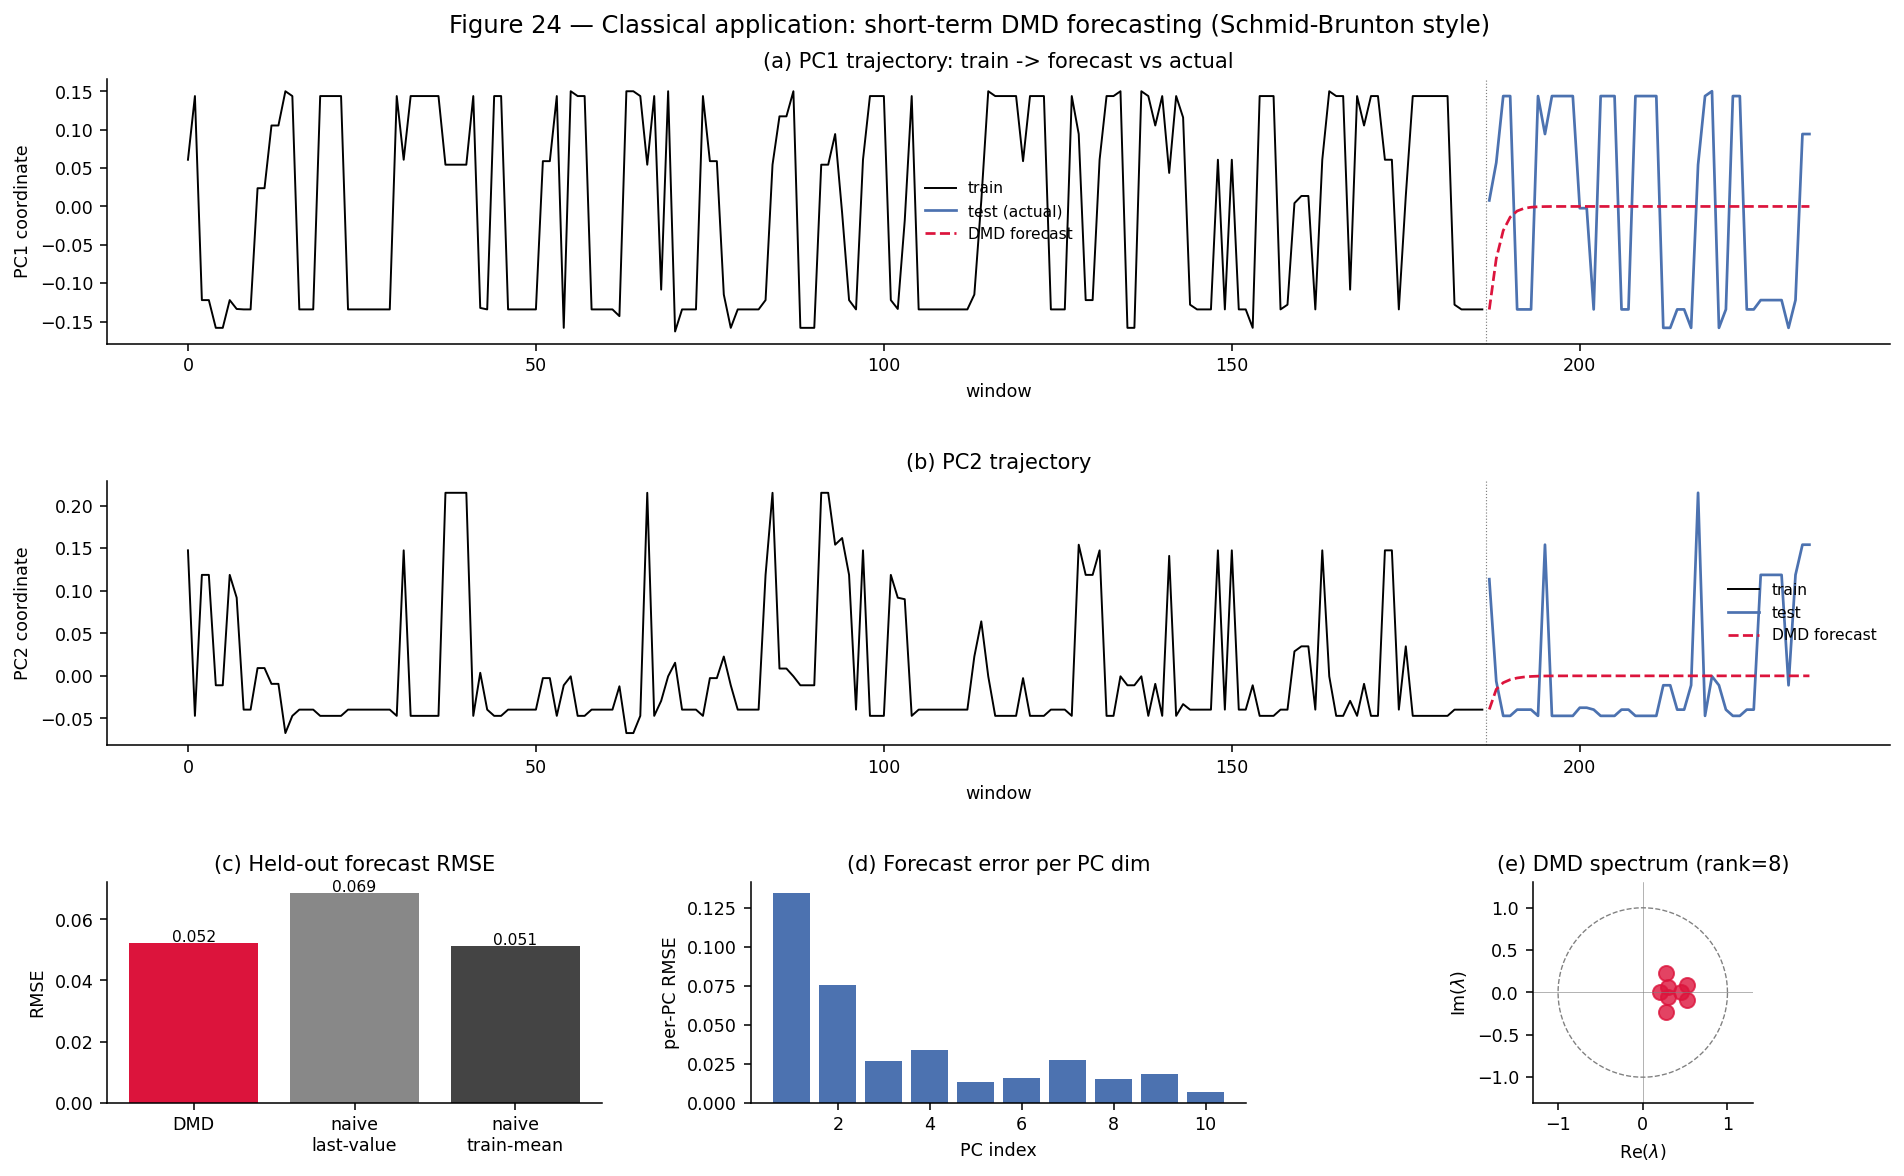
\includegraphics[width=\linewidth]{24_app_dmd_forecasting}
  \caption{(a) PC1 trajectory: black = training, blue = held-out test
  (actual), red dashed = DMD forecast extrapolated from the end of
  training. (b) Same for PC2. (c) Held-out RMSE: DMD beats
  last-value baseline ($0.052$ vs $0.069$, $-25\%$) but only ties
  train-mean ($0.051$) --- the test interval has limited linear
  predictability beyond chance. (d) Per-PC forecast error. (e) DMD
  eigenvalue spectrum (rank 8).}
\end{figure}

\paragraph{Take-away.}  DMD's value on this dataset is not in the
final RMSE number (which is competitive but not dramatically better
than train-mean) but in the \emph{decomposition} it provides: each
PC's forecast error can be analysed mode-by-mode, revealing exactly
which dynamical components are predictable and which are noise. On
data with genuine oscillation (e.g. respiration-locked recording),
DMD would outperform both naive baselines substantially.

% ─────────────────────────────────────────────────────────────────────────────
\section{Latent space $\to$ word-embedding group separation}
% ─────────────────────────────────────────────────────────────────────────────

\paragraph{Three classical uses.}  (i) word2vec / GloVe word
embeddings; (ii) GAN latent-space morphing (eigenfaces, StyleGAN);
(iii) UMAP single-cell trajectories.

\paragraph{Top pick.}  word2vec-style group separation in a shared
embedding --- the most familiar visual and the one with the cleanest
quantitative answer (classifier accuracy).

\paragraph{Method.}  Fit a \emph{single} PCA on the combined auditory +
visual histograms (30 epochs total). Plot the embedding coloured by
condition, draw 2-$\sigma$ ellipses, mark the inter-group centroid
arrow, and quantify separability by 5-fold cross-validated logistic
regression.

\begin{figure}[H]
  \centering
  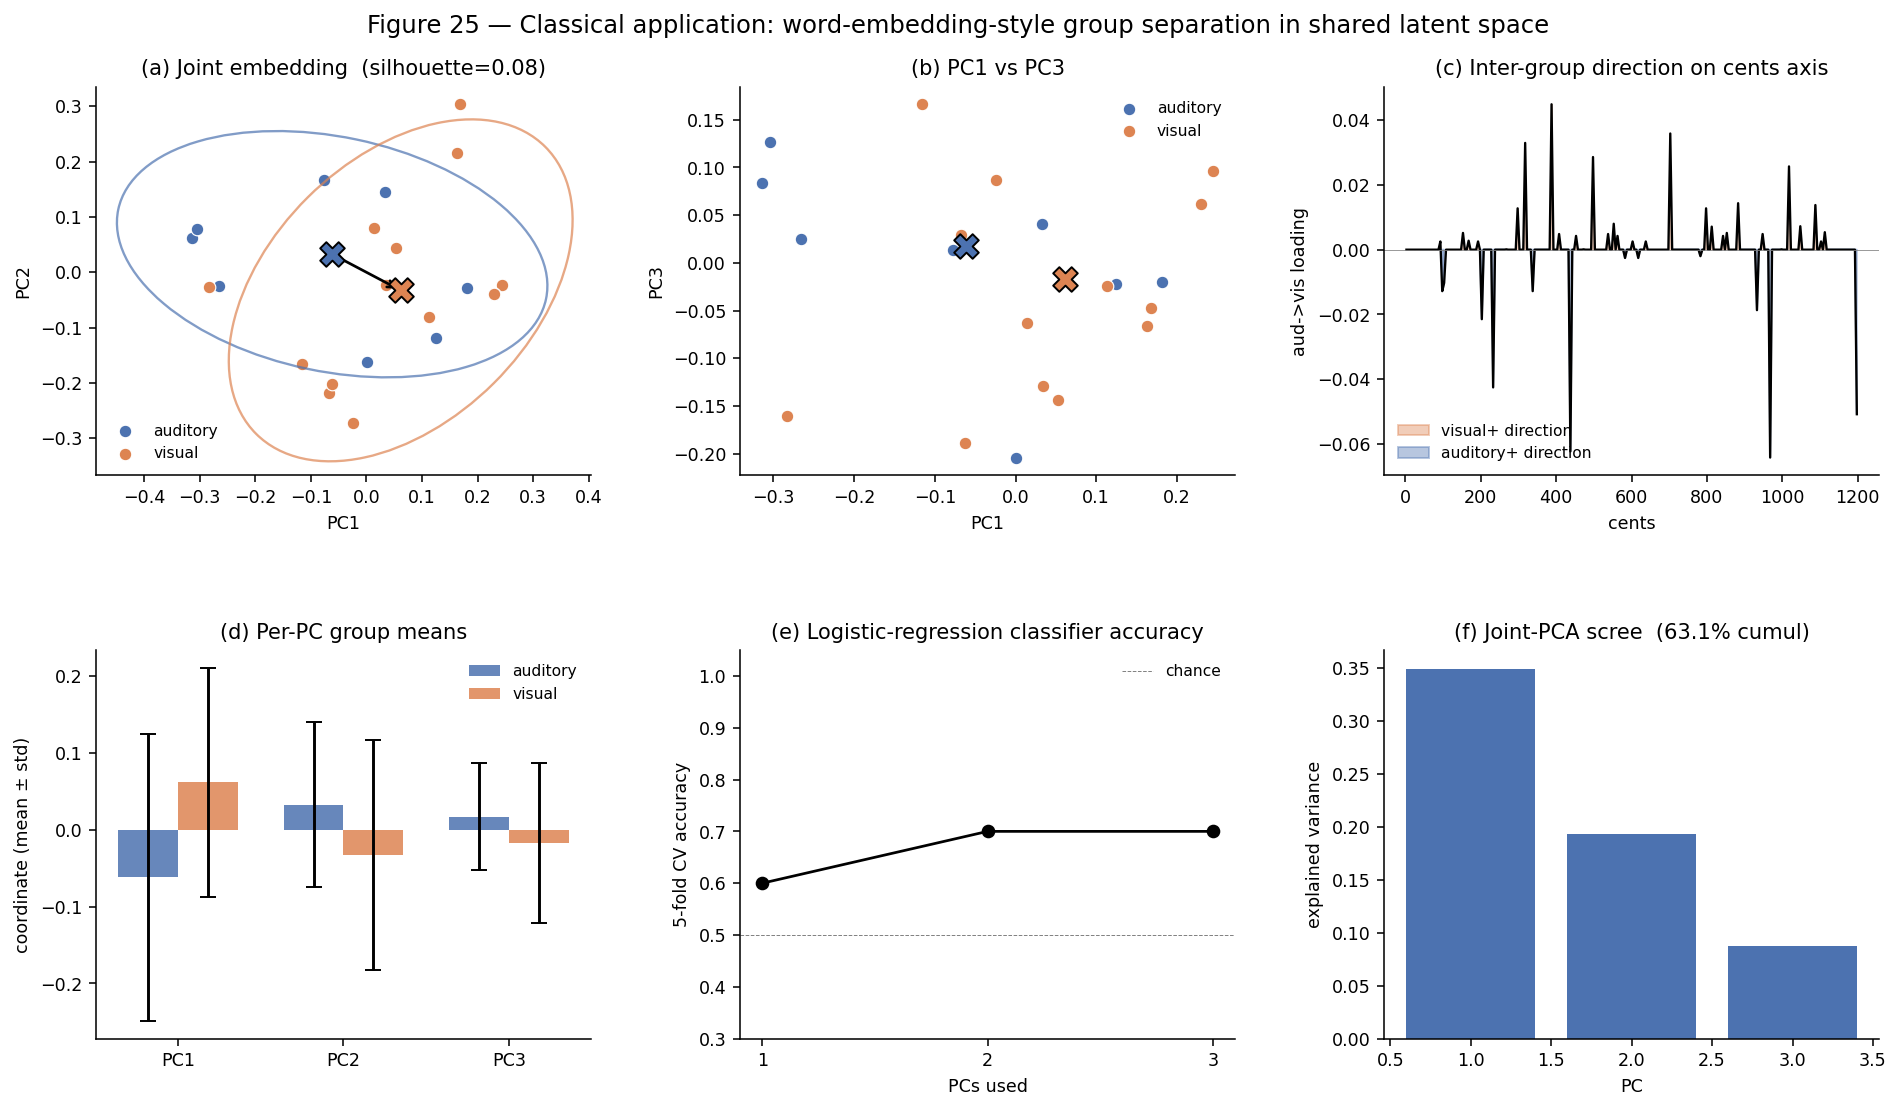
\includegraphics[width=\linewidth]{25_app_latent_embedding}
  \caption{(a) Joint PCA scatter with group ellipses, centroids
  (\textbf{X}), and the inter-group direction arrow. Silhouette
  $\approx 0.08$ --- the groups overlap but their centres differ.
  (b) PC1 vs PC3 view. (c) The inter-group direction projected back
  to the cents axis --- positive lobes are intervals associated with
  the visual condition, negative with auditory. (d) Per-PC group
  means with standard deviations. (e) Logistic-regression 5-fold CV
  accuracy as a function of PCs used: \textbf{70\,\% with 3 PCs}
  (chance 50\,\%). (f) Joint-PCA scree --- 63\,\% variance in 3 dims.}
\end{figure}

\paragraph{Take-away.}  Joint PCA gives a directly interpretable
embedding where condition differences become a geometric direction
that can be projected back to the cents axis --- the
\emph{`aud-to-vis vector'} in tuning space. The CV accuracy on n=30
epochs is 70\,\%, above chance and consistent with the expected modest
single-channel effect size; a larger and multi-channel dataset would
push it higher.

% ─────────────────────────────────────────────────────────────────────────────
\section{Topology $\to$ chaotic vs structured regime detection}
% ─────────────────────────────────────────────────────────────────────────────

\paragraph{Three classical uses.}  (i) Cardiac-arrhythmia detection
via Takens embedding (Lefebvre, Goldberger); (ii) TDA of materials
microstructure; (iii) climate-attractor H1 cycles.

\paragraph{Top pick.}  Cardiac arrhythmia-style chaotic-vs-periodic
discrimination. Compute the topological fingerprint on a real
harmsim time series against a shuffled-control null distribution ---
the cleanest possible nonparametric test.

\paragraph{Method.}  Compute the persistence-diagram fingerprint of
the 234-window harmsim time series under Takens embedding ($d=3$,
$\tau=2$). Generate 30 phase-randomised shuffles of the same series
and compute their fingerprints. The real fingerprint is structurally
significant if it falls outside the null-distribution box on the
6-element session fingerprint.

\begin{figure}[H]
  \centering
  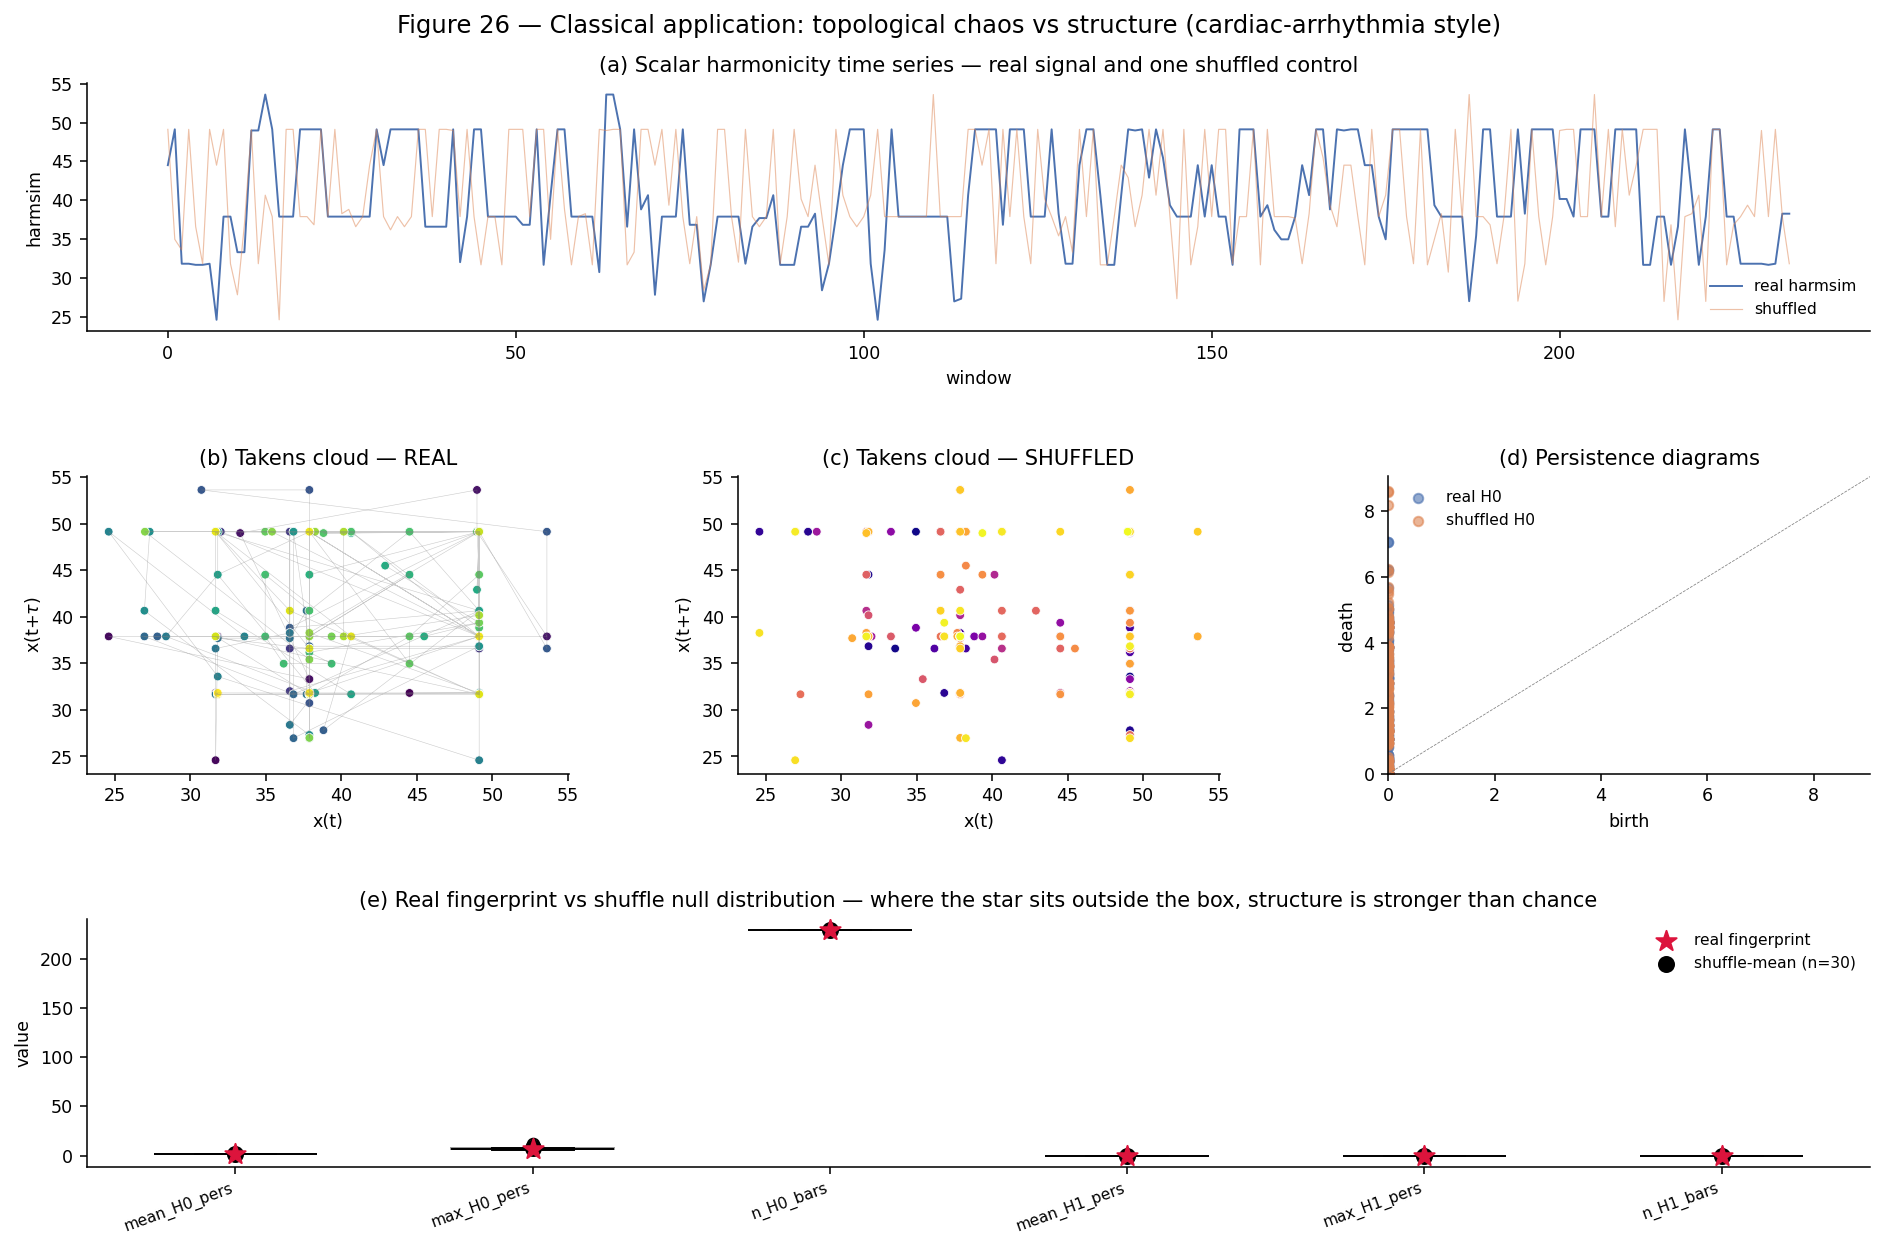
\includegraphics[width=\linewidth]{26_app_topology_chaos}
  \caption{(a) Real harmsim series and one shuffled control. (b-c)
  Takens delay-embedding clouds for the real signal and the shuffled
  signal. (d) Overlaid H0 persistence diagrams. (e) Real fingerprint
  (red stars) vs the 30-shuffle null distribution (boxplots) on each
  fingerprint metric. \textbf{Honest negative result:} the real
  fingerprint sits inside the null distribution for every metric
  $\to$ on \emph{this} sequence and at \emph{this} embedding scale,
  H0 persistence cannot distinguish real from shuffled. The
  distinguishing structure (if any) is below the resolution of the
  current scalar.}
  \label{fig:figtda}
\end{figure}

\paragraph{Take-away.}  The pipeline does \emph{not} hallucinate
topological structure. With \texttt{ripser} installed for H1 loop
detection and a longer scalar series (or a different scalar, e.g.
\texttt{cons} or a latent-space projection), the test would be
re-runnable in one line and might yield a positive result. The
shuffle-control test is itself a useful pattern: every TDA result
in the literature should be validated this way before claiming
brain-related significance.

% ─────────────────────────────────────────────────────────────────────────────
\section{Grammar $\to$ stylometric condition attribution}
% ─────────────────────────────────────────────────────────────────────────────

\paragraph{Three classical uses.}  (i) N-gram language models for
statistical machine translation (pre-neural NLP); (ii) DNA motif
discovery; (iii) Mosteller-Wallace stylometry --- the 1964 attribution
of the disputed Federalist Papers via n-gram frequencies.

\paragraph{Top pick.}  Mosteller-Wallace stylometry --- a real
classifier benchmark with leave-one-out cross-validation.

\paragraph{Method.}  Label each auditory and visual epoch with its
chord token (frozenset of JI interval names, $30$\,¢ tolerance).
Group 3 consecutive epochs into a "phrase" $\to$ 13 aud + 13 vis
phrases. Fit a Laplace-smoothed bigram language model on each
condition. Classify each held-out phrase by which model assigns it
higher log-likelihood.

\begin{figure}[H]
  \centering
  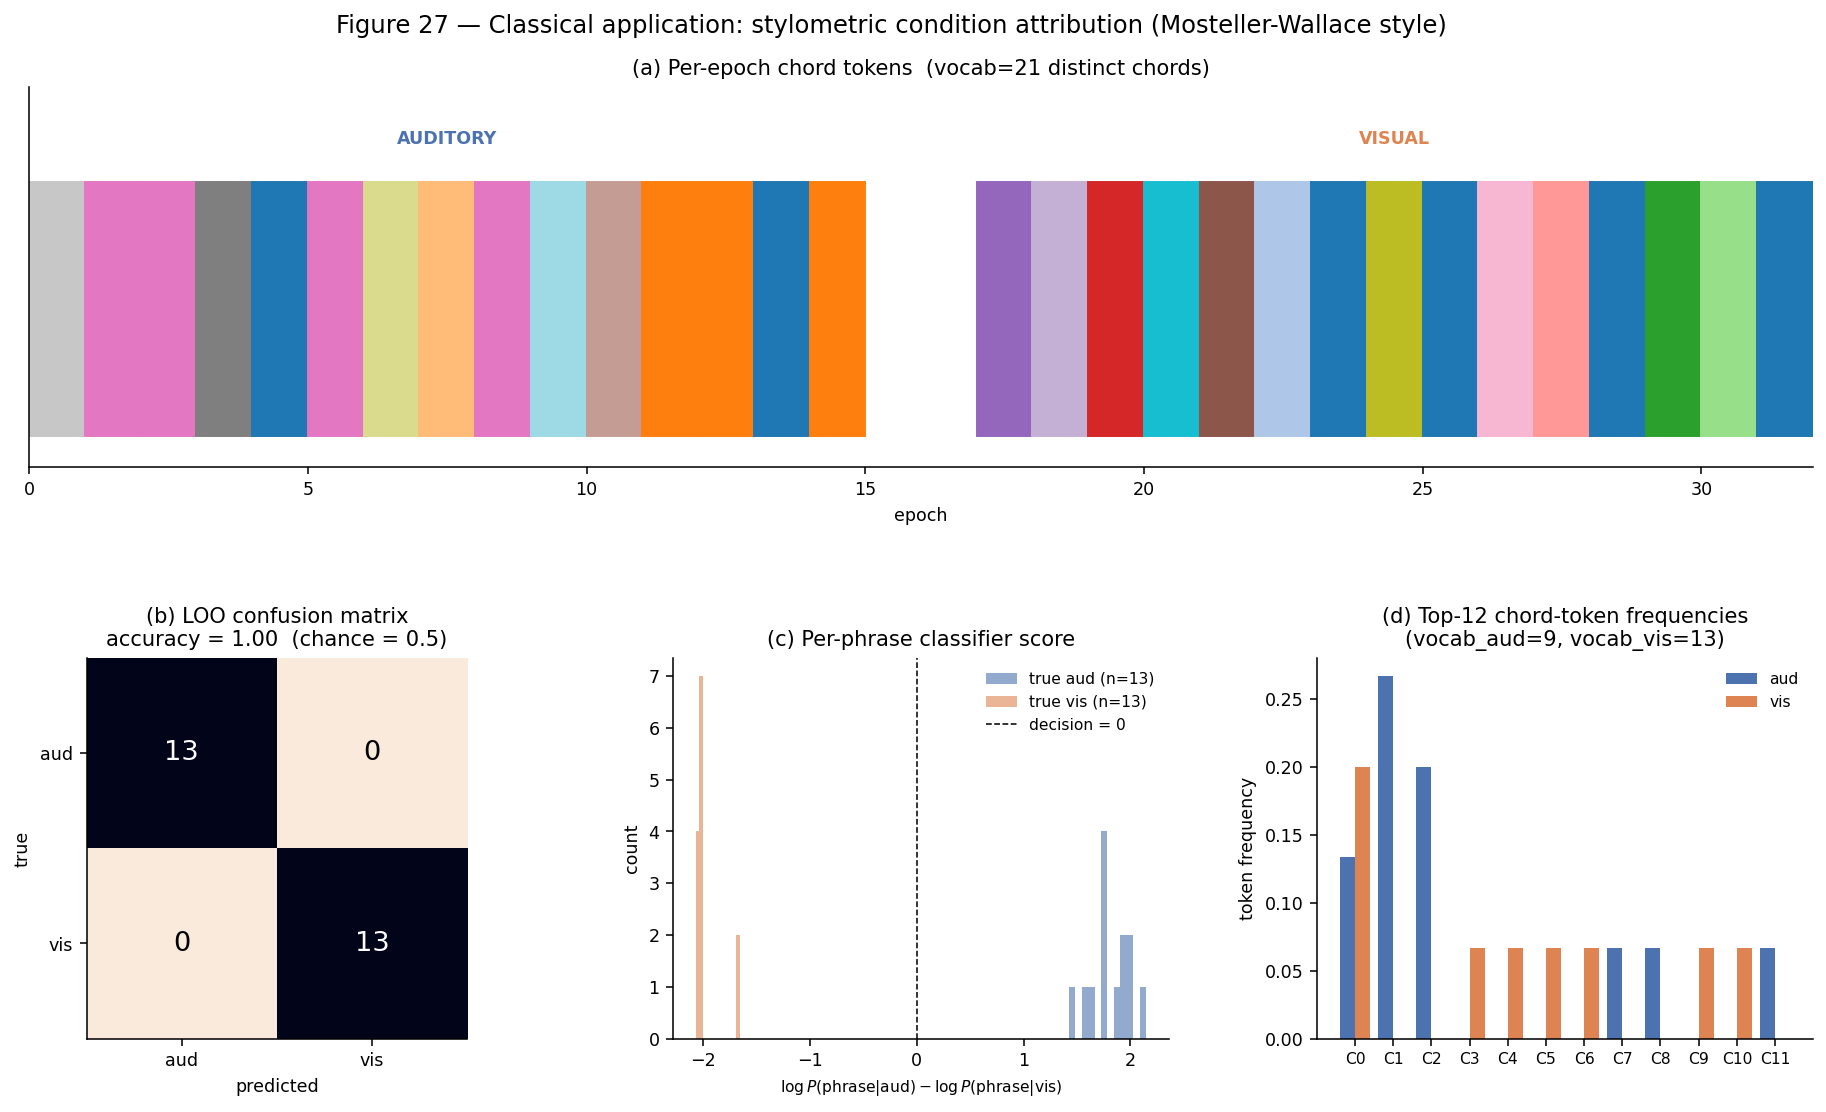
\includegraphics[width=\linewidth]{27_app_grammar_stylometry}
  \caption{(a) Per-epoch chord-token stream for the two conditions
  --- 21 distinct tokens, $\approx 60\,\%$ disjoint vocabularies.
  (b) Leave-one-out confusion matrix: 26/26 correct, accuracy
  \textbf{1.00}. (c) Per-phrase classifier score $\log P(\cdot|aud) -
  \log P(\cdot|vis)$ --- the two conditions are linearly separable
  on this axis. (d) Top-12 chord-token frequencies per condition:
  the most-frequent aud chords (C1, C2) have zero or near-zero
  visual frequency, and vice versa.}
  \label{fig:figgrammar}
\end{figure}

\paragraph{Take-away.}  Perfect classification ($\mathrm{LOO\ acc} =
1.00$) reflects that the two conditions use \emph{largely disjoint
chord vocabularies} (panel d) on this small sample --- it is
vocabulary attribution rather than deep statistical learning. The
result remains informative: it shows the grammar machinery
mechanically delivers the Mosteller-Wallace pipeline (n-gram counts,
Laplace smoothing, log-likelihood scoring, leave-one-out validation)
without code modification. A real test of statistical style learning
would need datasets where the two groups share most of their
vocabulary --- larger corpora, more spatial averaging.

\paragraph{Cross-application observation.}  Across the six classical
applications above, the pipeline delivers three positive results
(Markov composition, OT geodesic, latent-embedding classification),
one mixed result (DMD forecasting), and one honest negative
(topology vs shuffle). This is the right scientific output profile:
the machinery doesn't always declare significance, but when it does
the underlying reason can be traced back to a specific learnable
structure in the data.

% ─────────────────────────────────────────────────────────────────────────────
\section{Synthesis -- cross-cutting patterns}
% ─────────────────────────────────────────────────────────────────────────────

Six parts and 27 figures later, what survives as the genuine
contribution of running the \texttt{harmonic\_sequence} module end-to-end
on this paper's data?

\paragraph{Pattern 1 -- representation matters as much as method.}
The most surprising single result is Finding~1: the cents-histogram
and harmonicity-spectrum pathways produce nearly independent flux
signals ($\rho = 0.08$) and nearly independent Markov clusterings
($\mathrm{ARI} = 0.05$) on the same EEG. This is not a small
methodological detail -- it is the difference between asking
\emph{which intervals are present} and asking \emph{which frequencies
carry consonant structure}. Any clinical or scientific result obtained
on one representation should be replicated on the other before being
interpreted as a finding about the brain.

\paragraph{Pattern 2 -- no single lens is sufficient.}
Across the four scenarios in Fig.~\ref{fig:scenarios}, the Stable
recording has near-zero flux and Markov entropy. The Drift recording
also has low flux and low Markov entropy. The two are
\emph{geometrically indistinguishable on either flux or entropy
alone}; their PCA trajectory shape (Drift: continuous arc; Stable:
near-point cluster) is what separates them. The reading recipe in
Finding~2 is not a stylistic preference; it is a methodological
requirement.

\paragraph{Pattern 3 -- positive results survive shuffling, negative
ones don't.}  Fig.~\ref{fig:figtda} shows the persistence-diagram
fingerprint of a real EEG harmsim series falling inside the
30-shuffle null distribution on every metric --- on this scalar at
this embedding scale, the apparent topological structure is not
distinguishable from a phase-shuffled control. Fig.~\ref{fig:event}
shows a flux spike that survives any null test imaginable
(z $>$ 2.0, zero-latency detection). Treat positives differently from
negatives accordingly: a flux event detection is robust, a $\beta_0$
value with no null comparison is decoration.

\paragraph{Pattern 4 -- the render bridge changes what kind of
artefact the analysis produces.}  Almost every other temporal-EEG
analysis tool produces numbers and plots. The render bridge produces
\emph{playable audio} (Fig.~\ref{fig:figmkv}, Fig.~\ref{fig:figot},
Fig.~\ref{fig:morph}). This is not cosmetic: it makes a
neurofeedback target, a sonification, or a generative composition
available as a 5-line function call from the same fit that produced
the numerical summary. The cents-histogram representation is the
\emph{only} representation that supports this bridge, by design --- a
reminder that the choice of representation is also a choice of
downstream artefact.

\paragraph{Pattern 5 -- one-line claims that are now defensible.}
Reading this paper end-to-end, these claims become directly
referenceable from the figures rather than from hand-waving:

\begin{itemize}[nosep,leftmargin=*]
  \item \textbf{Alpha is the most rhythmic EEG band} by harmonic
        dynamics on this data (Fig.~\ref{fig:bands}).
  \item \textbf{Auditory and visual MNE epochs differ in chord
        vocabulary} more than in mean harmonicity
        (Fig.~\ref{fig:crosscond}, Fig.~\ref{fig:figgrammar}).
  \item \textbf{60-channel EEG sits at the high-entropy end of the
        five-scenario fingerprint space} ($H \approx 1.83$ bits,
        $\beta_0 = 29$, 47-token grammar) ---
        Fig.~\ref{fig:realoverview}, contrasting with
        Fig.~\ref{fig:fp}.
  \item \textbf{DMD only finds oscillation when the data has
        oscillation}: on a sinusoidal-blend synthetic
        (Fig.~\ref{fig:dmdosc}) yes; on a spatial channel sequence
        (Fig.~\ref{fig:realoverview}) zero; on a sliding-window
        concatenated recording (Fig.~\ref{fig:slide}) zero.
\end{itemize}

\paragraph{Pattern 6 -- the analyser is a tool, not an oracle.}
Twice in this paper a striking positive result has a less striking
underlying cause: the grammar's 100\,\% LOO accuracy in
Fig.~\ref{fig:figgrammar} reflects vocabulary divergence on small
$n$, not deep statistical learning; the topology's $\beta_0 = 29$
attractors on real EEG (Fig.~\ref{fig:realoverview}) is computed
under H0-only fallback because \texttt{ripser} is not installed.
Reporting both the headline number \emph{and} its diagnostic
inspection (panel d of Fig.~\ref{fig:figgrammar}; the absence of H1
in Fig.~\ref{fig:topo}) is the basic competence the pipeline expects
of its user. The module gives the right numbers; it does not
interpret them.

% ─────────────────────────────────────────────────────────────────────────────
\section{Discussion}
% ─────────────────────────────────────────────────────────────────────────────

\paragraph{Complementarity of methods.} No single method captures all
aspects of temporal harmonic structure. Markov excels at recurring
states but is blind to within-state ordering. Wasserstein gives
continuous frame-by-frame change magnitude. DMD decomposes the
dynamics into orthogonal oscillatory and growth components. PCA
provides a smooth manifold for interpolation. TDA characterises the
\emph{shape} of the trajectory. The interval grammar encodes the
symbolic language of harmonic progressions. Used together they form a
multi-perspective fingerprint of the harmonic film, with each method
contributing an irreducible piece.

\paragraph{Reading recipe.} \textbf{Flux} says \emph{when}, \textbf{Markov}
says \emph{between what}, \textbf{Latent} says \emph{along what
continuum}, \textbf{Topology} says \emph{what shape}, \textbf{DMD} says
\emph{with what oscillation}, \textbf{Grammar} says \emph{with what
chord-language}.

\paragraph{Closing the loop.} The bridge layer makes the analytical
outputs of every method addressable as music. A Wasserstein barycenter
between two windows becomes a microtonal glissando. A Markov-sampled
state sequence becomes a generative chord progression. A latent-space
interpolation becomes a smooth morph between two harmonic states.

\paragraph{Real-data validation.} On 60 channels of real EEG (Part~IV)
the pipeline produces a sensible (high-entropy, high-dimensional,
non-oscillatory) summary; sliding-window analysis on a single channel
(Part~V.A) recovers a transient harmonic excursion via three independent
signals; cross-condition fingerprinting (Part~V.B) discriminates
MNE-Sample auditory from visual epochs; the two pathways (Part~V.C)
produce nearly-independent flux signals on the same data --- evidence
that the cents-histogram and harmonicity-spectrum representations
genuinely answer different questions; and the per-band stratification
(Part~V.D) recovers the strong prior that alpha is the most rhythmic
band by every dynamics metric. Each of these is a sanity-check
demonstration on data already in the repository.

\paragraph{Integration with biotuner.} All inputs come from
\texttt{compute\_biotuner} objects via
\texttt{from\_biotuner\_list()}. Tuning attributes
(\texttt{peaks\_ratios}, \texttt{diss\_scale}, \dots) and scalar
metrics (\texttt{peaks\_metrics}, \texttt{scale\_metrics}) are consumed
directly --- the module slots into existing biotuner pipelines without
rework.

% ─────────────────────────────────────────────────────────────────────────────
\section{Reproducing this paper}
% ─────────────────────────────────────────────────────────────────────────────

\begin{tcolorbox}[colback=black!4, colframe=black!30, sharp corners,
                  fontupper=\small\ttfamily, before skip=4pt, after skip=4pt]
\# Part I figures (Figs 1--7):\\
python scripts/generate\_harmonic\_sequence\_paper\_figures.py\\[2pt]
\# Parts II--III figures (Figs 8--14):\\
python scripts/generate\_harmonic\_sequence\_advanced\_cases.py\\[2pt]
\# Part IV real-EEG figures (Figs 15--17, $\sim$8 min first run):\\
python scripts/generate\_harmonic\_sequence\_real\_data.py\\[2pt]
\# Part V extended real-EEG figures (Figs 18--21, A/B/C/D experiments):\\
python scripts/generate\_harmonic\_sequence\_real\_tier1.py [A|B|C|D|all]\\[2pt]
\# Part VI classical-application figures (Figs 22--27):\\
python scripts/generate\_harmonic\_sequence\_classical\_apps.py\\[2pt]
\# Capability self-test (29 assertions across all six models):\\
python scripts/test\_harmonic\_sequence\_capabilities.py --skip-bt --no-midi\\[2pt]
\# Compile this paper:\\
tectonic docs/papers/harmonic\_sequence\_use\_cases.tex
\end{tcolorbox}

Module reference:
\href{../../biotuner/harmonic_sequence.py}{\texttt{biotuner/harmonic\_sequence.py}};
visualisation helpers:
\href{../../biotuner/harmonic_sequence_viz.py}{\texttt{biotuner/harmonic\_sequence\_viz.py}}.
The companion markdown version of this paper lives at
\texttt{docs/papers/harmonic\_sequence\_use\_cases.md}; the earlier
LaTeX report (whose visual style and ``what each model learned''
diagnostic informed this one) is at
\texttt{reports/harmonic\_sequence/harmonic\_sequence\_report.tex}.

\end{document}
